\chapter{MGS}

MGS is a C++  graph-based modeling framework. The input to the system is a
scripting language called {\bf GSL} (Sect.\ref{sec:GSL-how-it-works}).

GSL : the script that helps to connect different C++ classes together in
a graph-based simulator system. (Chap.\ref{chap:MGS-GSL})

Any component in MGS needs to belong to certain category
(Sect.\ref{sec:MGS-components}). To help writing code conforms to MGS framework,
another scripting language was used MDL : the script that helps generating C++
classes that conform to MGS  code standard (Chap.\ref{chap:MGS-MDL})
  
 
  
\section{Tutorial: Graph-based simulation}
\label{sec:graph-based-simulation}

The core of the graph-based simulation is saved in 2 folders:
\verb!gsl! and \verb!mdl!.

\begin{verbatim}
nts/
   gsl/
   mdl/
   models/      (where developed *.mdl files reside)
   graphs/      (where developed *.gsl files reside)
   nti/         (code for NTS purpose)
   common/      (where common utilities code reside)
   datasheets/ 
\end{verbatim}

The software has 3 components
\begin{enumerate}
  \item GSL (Sect.\ref{sec:GSL}): 
  This is known as MGS (Model-Graph Simulator) - \verb!gslparser! executable
  file that can parse script written in GSL language to define graph
  connection.
  
  Components in a graph can be one of the following forms (Sect.\ref{sec:graph-components}).
  Regardless of the form, at the code-level, they are implemented in the form of
  a C++ classes. In order to help the MGS framework to be able to 'connect' them
  together, i.e. mapping memory references from one instance to another,
  there is a need for several helping classes; which follows a given code
  design of class hierarchy.
  
  As all of these helping classes follow a given design patterns; they can be
  code-generated. A scripting language - called MDL - has been developed to
  facilitate that process.
  
  \item MDL (Sect.\ref{sec:MDL}): MDL scripting language is designed to help
  generating helping classes for any C++ class to be usable as a
  MGS-based graph-component.
  
  \verb!mdlparser! executable   file that can parse the script written in MDL
  language to define models, and generated C++ code stub, which then can be used
  in GSL.
  
  
  \item NTS (Sect.\ref{sec:TissueFunctor}): a set of components implemented
  using MDL and GSL that allows the incorporating .swc files into the graphs
  to perform the simulation in the computational neuroscience domain.

\end{enumerate}


This section goes through a number of examples on how to use the
NTS system.

Steps for every project
\begin{enumerate}
  \item write .mdl script if a new graph-based component is needed (i.e.
  NodeType, VariableType, ConstantType)
  
  \item write the .gsl script, e.g. \verb!models.gsl!, that combines all these
  graph-based components in a proper way
  
  \item run the simulation
\begin{verbatim}
mpiexec -n 8  <path-to>/gslparser models.gsl
\end{verbatim}

\end{enumerate}


\subsection{Graph's components}
\label{sec:graph-components}

We focus on the NodeType (Sect.\ref{sec:NodeType-GSL}).

Suppose nodetype \verb!AMPAReceptor! has the class
\begin{verbatim}
class CG_AMPAReceptor : public DimensionArrayProducer, 
                        public IndexArrayProducer,
                        public BranchDataArrayProducer
{
}
\end{verbatim}




\subsection{How the MGS framework works?}
\label{sec:MGS-how-it-works}

MGS enables the user to define a time-step based simulation system (TSBSS).
The TSBSS is defined in a *.gsl file (Sect.\ref{sec:GSL-script}).
To understand how the simulation works, read
Sect.\ref{sec:GSL-how-it-works}.
The system is represented as a graph-based system with different components
interconnected to each other.

There are different kinds of component that can be used in a TSBSS
(Sect.\ref{sec:MDL-component}). The code for each component (e.g. Node) follows
certain pattern that can be code-generated if we can describe what kinds of data
the component expose (via \verb!Implements! keyword), and what are the phase
kernels (e.g. InitPhase, RuntimePhase), for each phase, what kinds of data to be
synced (to the proxy, if present, by passing the data as the arguments to the
phase kernel); and how it references to data on another component (via incoming
connection). All of these are described in the MDL (e.g. LifeNode), example

{\tiny
\begin{verbatim}
Interface ValueProducer {
   int *value;
}
Node LifeNode Implements ValueProducer {
   int value;
   int publicValue;
   int* [] neighbors;

   InitPhase initialize;
   RuntimePhase update();
   RuntimePhase copy(publicValue);

   ValueProducer.value << &publicValue; /* this line define what data attribute
                                        of the node is available for other node
                                        to access 
                                        */
}
\end{verbatim}
}

Using the \verb!mdlparser! binary, the generated code is copied to a folder of
the same name in the \verb!./gsl/extension/<component>/!,
\begin{verbatim}
./gsl/extension/node/LifeNode
\end{verbatim}

Inside this folder, we have \verb!src! and \verb!include! subfolders which holds
a number of classes which are related to each other via a
a hierarchical structure in which two main classes are the LifeNode classs and
LifeNodeCompCategory class. The other classes are supporting classes (i.e.
code-generated classes) that can help the MGS framework to get access to the
underlying data of LifeNode and LifeNodeCompCategory.

\begin{verbatim}
./gsl/extension/node/LifeNode/src
./gsl/extension/node/LifeNode/include
\end{verbatim}

Here, we describe how the MGS framework connect different components together.
Any component in a graph-based system (e.g. Node, Variable, Constant)
communicate to each other via one's provided service. Here, a service refers to
a particular data member of a given component that can be accessed from another 
component (Sect.\ref{sec:Service}).

Each component is used as a class, so its data member are exposed to MGS in the
form of service (Sect.\ref{sec:Node-data-member-as-a-service}).
To manage different Services of a graph's component, e.g. LifeNode for example,
a Publisher (Sect.\ref{sec:Publisher}) is generated for that graph's component,
e.g.
\verb!CG_LifeNodePublisher! class (Sect.\ref{sec:CG_xxxPublisher}).

If a component want their data to be accessible from another component, it
needs to expose via an interface (Sect.\ref{sec:MDL-Interface}). Then, we map
the data to the interface using \verb!<<! operator in the MDL code
\begin{verbatim}
  // here it exposes the address of the data member
ValueProducer.value << &publicValue;
\end{verbatim}

Example: The generated code enables the accessing of the proper data member,
given the Interface name and the Interface's data member
{\tiny
\begin{verbatim}
std::string CG_LifeNodePublisher::getServiceNameWithInterface
                 (const std::string& interfaceName, 
                 const std::string& subInterfaceName) 
{
   if (interfaceName == "ValueProducer") {
      if (subInterfaceName == "value") {
         return "publicValue";
      }
   }
   return "";
}
\end{verbatim}
}

\subsection{-- MGS: multiple layers of abstraction}
\label{sec:MGS-multiple-layer-of-abstraction}

MULTIPLE LAYERS OF ABSTRACTION: With the different supporting classes (prefix
\verb!CG_!), it enables one class, representing a model component, to be able to
communicate with other classes, representing other model components. In
particular, the class goes through 3 or 4 layers of abstraction that coordinate
the communication between them, regardless of class's definition, and processes
on which the class's object runs, Fig.\ref{fig:NTS_code-layers}.

NOTE: The Interface component only goes through 3 layers, as it has no code body
implementation. The classes generated from 'Interface' component works as proxy
for communication between instances from two different classes.

\begin{itemize}
  \item 2 layers for generated code from MDL 
  
  \item 2 layers for codes defined in the MGS frameworks to handle the
  communication between generated codes at different hardware level, i.e.
  shared-memory processors or distributed-memory processors.
\end{itemize}

\begin{figure}[hbt]
  \centerline{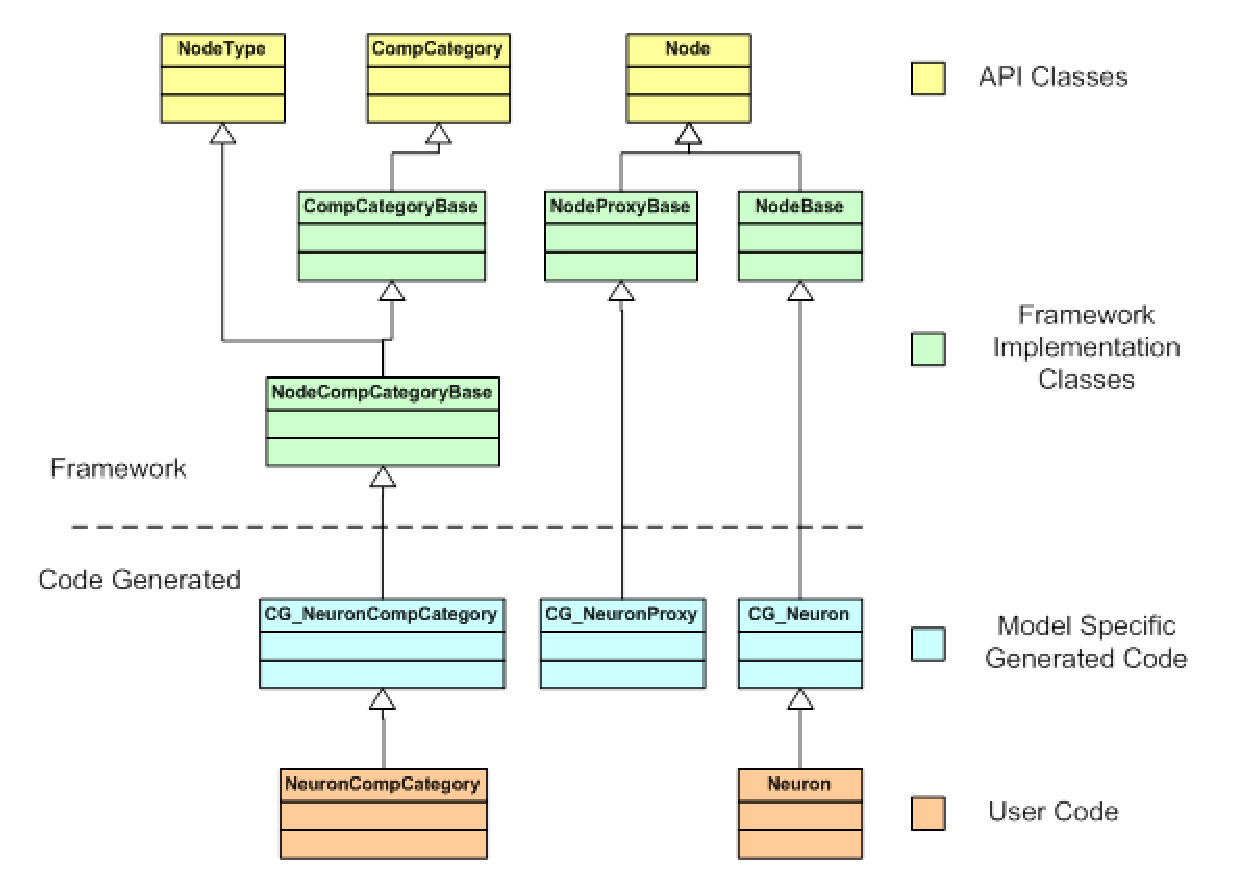
\includegraphics[height=5cm,
    angle=0]{./images/NTS_code-layers.eps}}
\caption{Layers of code in a model}
\label{fig:NTS_code-layers}
\end{figure}



% How about Interface? as a service (i.e. the Node's data member -
% Sect.\ref{sec:Node-data-member-as-a-service}) is exposed via the interface,
% another method is defined to enable the accessing of the proper data member,
% given the Interface name and the Interface's data member.

\subsection{-- MGS: distributed system}
\label{sec:MGS-distributed-system}

The whole world, as defined in GSL may not fit a single MPI process, i.e. only a
portion of the world is handled by the current MPI process. Such a portion is
called a granule (Sect.\ref{sec:Granule}). To help dividing the 'world' into
granule, a proper granule mapper to support granule mapping has to be used
(Sect.\ref{sec:GranuleMapper}).

Another important part of the graph-based simulation is how the different
instances of the same node-type, or from different node-type connect to each
other, i.e. access the data from each other. Then we need to use connector
functor (Sect.\ref{sec:connector-functor}).


\subsection{Game of Life}
\label{sec:nts-example-game-of-life}

Here, you want to have a 2D map of cells, each cell can get value 0 or 1,
depending upon the sum of its 4 neighbors' values.
\begin{itemize}
  \item sum $\le$ sparseValue: make the cell alive, i.e. set 1
  \item sum $\ge$ crowdedValue: kill the cell, i.e. set 0
\end{itemize}
Each node can live or die (i.e. represented by one data member with two
possible values 0 or 1), and this value changes after each iteration, depending
on how many alive neighbors.

\subsection{* GSL script}

Briefly, the highest level of abstraction in GSL is Repertoire
(Sect.\ref{sec:GSL-repertoire}). The system performs the simulation by looking
at first the 'root' Repertoire.
Suppose you have one or more directed graphs: how to know which one is the root
Repertoire. The context-based GSL scriptting language helps identify the root
Repertoire. Most of the time, we only have one grid in the system
(Sect.\ref{sec:Grid}).

The 2D map is represented as a Grid with certain properties, which is
represented by a class named World, and then we define an object name myworld of
this class. The GSLparser will recognize and automatically perform the
simulation, until it stops (Sect.\ref{sec:GSL-when-to-stop}).

\begin{figure}[hbt]
  \centerline{
  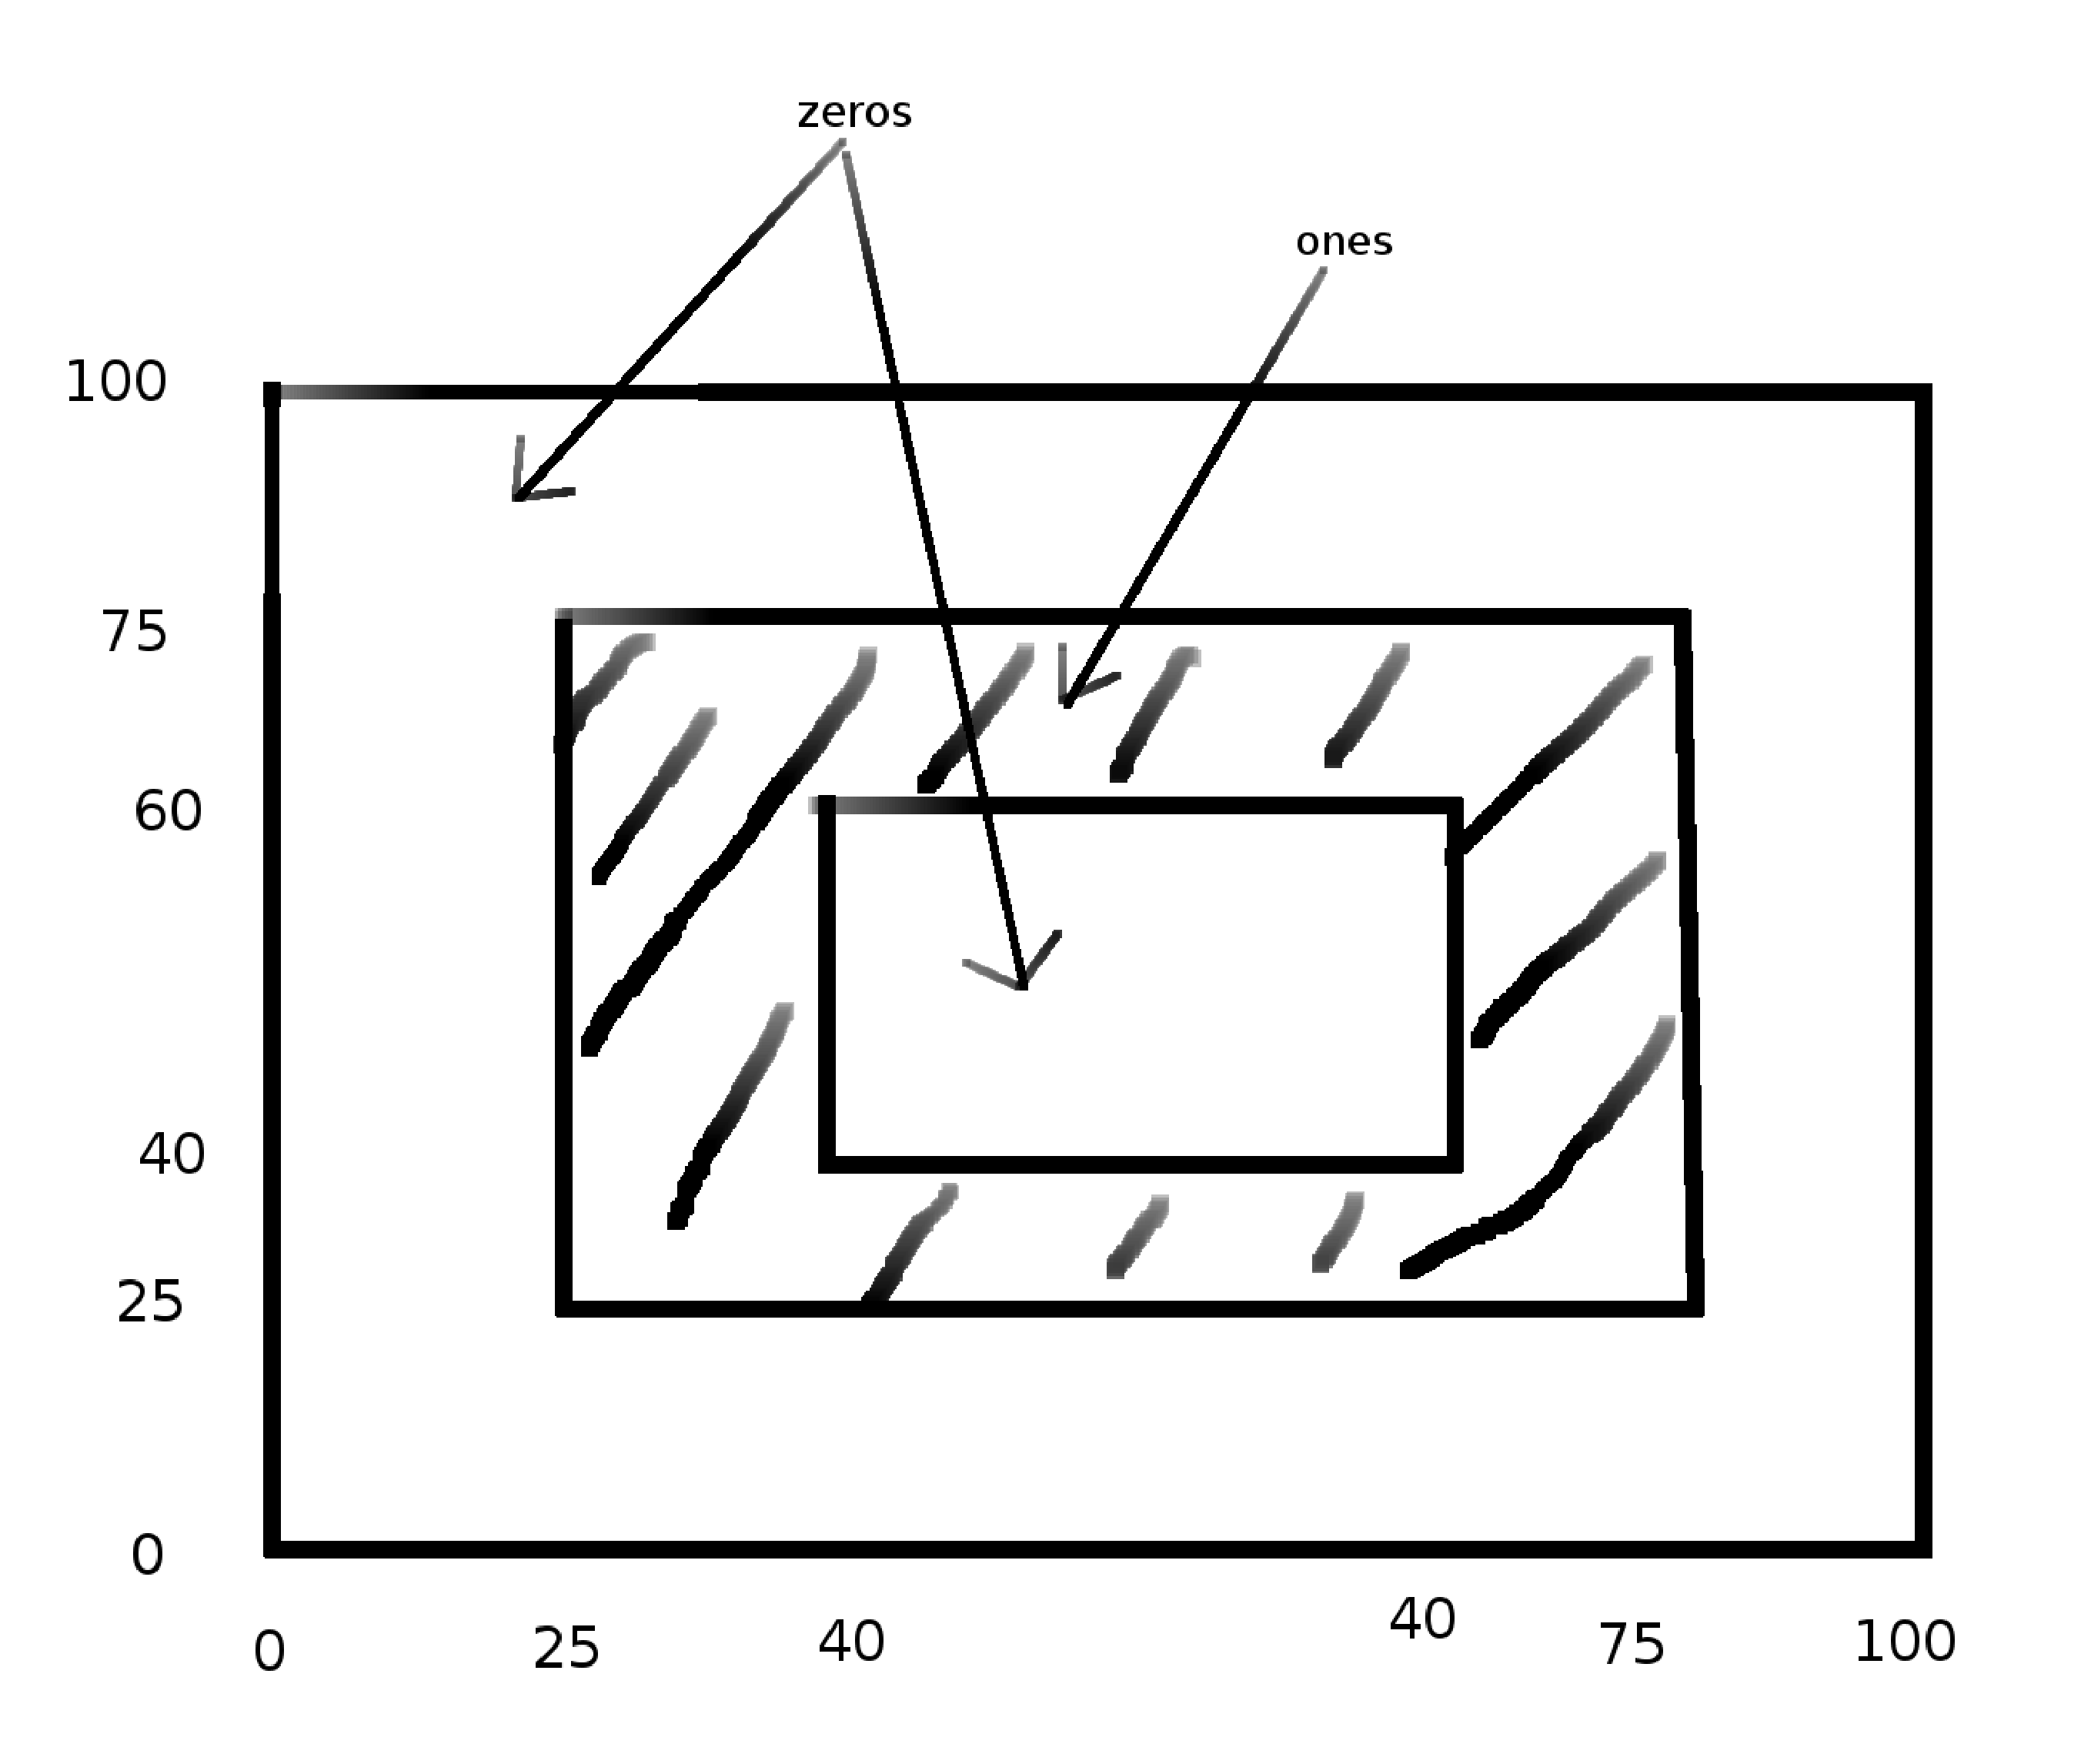
\includegraphics[height=7cm,
    angle=0]{./images/game-of-life-initial-configuration.eps}}
\caption{Size of the grid (100 x 100) and initial configuration of the Game of
Life} \label{fig:game-of-life-initial-configuration}
\end{figure}

\begin{verbatim}
Grid World
{
  ...
}

World myworld;
\end{verbatim}

Each grid has a given dimension, defined using \verb!Dimension()! statement.

{\small
\begin{verbatim}
// A grid is a collection of layers (GridLayerDescriptors.                                                                                   
// The dimensions of the grid is set at construction, however each layer                                                                     
// may have its own density.                                                                                                                 
// What it looks like, the main responsibility of the grid is to figure                                                                      
// out how to map node coordinates to one dimensional coordinates(nodeIndex)                                                                 
// and vice versa.                                                                                                                           
// It also keeps track of the maximum and the minimum densities out of                                                                       
// all the layers it has.                                        
\end{verbatim}
}
\verb!./gsl/framework/parser/include/Grid.h! file


There can be as many layers mapping on the grid as you want, using Layer()
statements. Each Layer only contains instances of a given node-type only.
Here, we have a layer that contains instances of NodeType node-type.
We want to have one layer of LifeNode node-type uniformly distributed to every
cell with 1 instance of NodeType per cell. 
\begin{verbatim}
Grid World
{
  Layer (nodes, LifeNode, UniformLayout(1), <nodekind="Nodes">)
}
\end{verbatim}

Here, {\it UniformLayout} is a functor (Sect.\ref{sec:UniformLayoutFunctor}).
You will uses functors a lot to modify the behavior of the graph, to help organizing the functors to know if using a
functor at one place in the script is proper or not, we try to put a category
information to them, so that it can be checked. There are currently 11 different
categories of functors (Sect.\ref{sec:functors-in-MGS-framework}).


\label{sec:GameofLife-GSL-InitNodes}
Each cell is identified by its lower-left coordinate
(x,y). The initial configuration is given in
Fig.\ref{fig:game-of-life-initial-configuration}.
{\it
\begin{verbatim}
Grid World
{
  InitNodes (.[25:75,25:75].Layer(nodes), Same( Pset<LifeNode, NodeInit> )  (<value=1>) );
  InitNodes (.[40:60,40:60].Layer(nodes), Same( Pset<LifeNode, NodeInit> )  (<value=0>) );
  
}
\end{verbatim}
}

In a directed graph, node A does not need to know which nodes it connect to, but
node B needs to know which nodes it receives the input.
\begin{verbatim}
A ------> B
\end{verbatim}


Now, we need a LifeNode nodetype, so we use MDL to help creating this LifeNode
(Sect.\ref{sec:MDL-script-game-of-life}). The basic component of a graph is a
node. However, in addition to this, there can be other components. GSL system
defines 7 different components (Sect.\ref{sec:GSL-extension}). The MDL system
(Sect.\ref{sec:MDL}) is designed to help generating code for user-defined
components belonging to one of these components using MDL script
(Sect.\ref{sec:MDL-script-structure}).


\subsection{* MDL script}
\label{sec:MDL-script-game-of-life}

\begin{enumerate}
  
  \item write *.mdl script: File.mdl (Sect.\ref{sec:MDL-script-structure})
 and put them into \verb!./models/<ProjectName>/File.mdl!
  
Here: Create Life.mdl file written in MDL scripting language
  (Sect.\ref{sec:MDL-script})

  
  \item compile the script

\begin{verbatim}
cd ./models/<ProjectName>/
$NTSROOT/mdl/bin/mdlparser File.mdl
\end{verbatim}  
  
Here:
\begin{verbatim}
cd ./models/Life/
$NTSROOT/mdl/bin/mdlparser Life.mdl
\end{verbatim}  
Once the script complete, it also generate a number of C++ files and folders
inside the project folder. For example: GameofLife project
(Sect.\ref{sec:nts-example-game-of-life})

\begin{verbatim}
copyModules  
Extensions.mk  
LifeDataCollector/  
Life.mdl  
LifeNode/  
ValueProducer/
\end{verbatim}

and then it automatically runs the script \verb!copyModules! to copy these
folders (containing C++ generated code) to the appropriate location in the \verb!./gsl/extension/!
\begin{verbatim}
./gsl/extension/interface/ValueProducer/
./gsl/extension/node/LifeNode/
./gsl/extension/variable/LifeDataCollector/
\end{verbatim}
  
  \item jump to the different folders where the generated codes are copied where
  the C++ code for the different components in the above script are generated, and modify them accordingly
  
\end{enumerate}


\verb!LifeNode! will be used as a node that can connect to other \verb!LifeNode!
and share the data via the Interface \verb!ValueProducer!'s data of \verb!int!
type (here we use pointer as we want direct reference and no data copy).
All \verb!LifeNode! instances reference to some common data, which is called
Shared data. 

{\tiny 
\begin{verbatim}
Interface ValueProducer {
   int *value;
}

/* If a node want to share it data with other components
   it needs to specify these data via the form of Interface
   
   Here, LifeNode can expose data via the ValueProducer interface
*/
Node LifeNode Implements ValueProducer {
   int value;
   int publicValue;
   int* [] neighbors;

   Shared {
     int habitable;
     int tooSparse;
     int tooCrowded;
   }

   InitPhase initialize;
   RuntimePhase update();
   RuntimePhase copy(publicValue);

   ValueProducer.value << &publicValue; /* this line define what data attribute
                                        of the node is available for other node
                                        to access 
                                        */

   /* This defines how a node is connected to another node 
      Inside () we can define the predicate, i.e. the condition on which the
      connection is established (here we ignore).
      
      And what Interface it expects from the connected node, e.g.
      ValueProducer interface. With this interface, what data it will get 
      (i.e. 'value'), and where it will store (i.e. an element in the
      array 'neighbors')
    */
   
   Connection Pre Node () Expects ValueProducer {
      ValueProducer.value >> neighbors; /* this line defines how the data from
                                        other nodes are collected. The data
                                        attribute to store is typically an array
                                        as it can get from multiple connected
                                        nodes.
                                        The size of this array is equal to the
                                        number of connected nodes and is
                                        determined at the time of the simulation
                                        setup in GSL stage. So we just use []
                                        
                                        */
   }
}

Variable LifeDataCollector
{
   string fileName;
   CoordsStruct [] coordsArray;
   int* [] vals;

   InitPhase initialize;
   TriggeredFunction dataCollection;
}
\end{verbatim}
}

The Node names and Variable names will be put into the appropriate folders
\begin{verbatim}
$NTSROOT/gsl/extensions/node/
$NTSROOT/gsl/extensions/variable/
\end{verbatim}

Example: inside these folders are generated code that you need to modify
\begin{verbatim}
$NTSROOT/gsl/extensions/node/LifeNode/
         ... include/
         ... src/
         ... obj/
$NTSROOT/gsl/extensions/variable/LifeDataCollector/
         ... include/
         ... src/
         ... obj/
\end{verbatim}



\subsection{* generated C++ code: node/compcategory}
\label{sec:MGS_user-defined-class-nodetype-compcategory}

Sec.\ref{sec:CompCategoryBase} discusses NodeCompCategoryBase.
\begin{verbatim}
LifeNodeCompCategory
  |
  +- CG_LifeNodeCompCategory
       |
       friend CG_LifeNodeCompCategory
       +- NodeCompCategoryBase
            |
            +- DistributableCompCategoryBase
            +- NodeType
                |
                +-         
       
\end{verbatim}

\subsection{* generated C++ code: node}
\label{sec:MGS_user-defined-class-nodetype}

As we define a Node name \verb!LifeNode!, there will be C++ code generated for
this node. 
\begin{verbatim}
LifeNode
  |
  +- CG_LifeNode
       |
       friend CG_LifeNodePublisher
       friend LifeNodeCompCategory
       friend CG_LifeNodeCompCategory
       +- <interface classes>
       +- NodeBase
            |
            +- Node
                |
                +-         
                  NodeDescriptor, 
                  ServiceAcceptor,
                  TriggerableBase
\end{verbatim}


Here, \verb!NodeBase! is the class with important methods that we often use at
C++ code level (Sect.\ref{sec:NodeBase}).



We ignore \verb!CG_*! files, and need to modify 
\verb!LifeNode.h.gen! \verb!LifeNode.C.gen!

{\tiny
\begin{verbatim}
tmhoangt:/home/tmhoangt/nts>vi gsl/extensions/node/LifeNode/include/
CG_LifeNodeCompCategory.h        CG_LifeNodeProxyDemarshaller.h   CG_LifeNodeWorkUnitInstance.h
CG_LifeNodeFactory.h             CG_LifeNodeProxy.h               CG_LifeNodeWorkUnitShared.h
CG_LifeNodeGridLayerData.h       CG_LifeNodePSet.h                LifeNodeCompCategory.h
CG_LifeNode.h                    CG_LifeNodePublisher.h           LifeNodeCompCategory.h.gen
CG_LifeNodeInAttrPSet.h          CG_LifeNodeSharedMembers.h       LifeNode.h
CG_LifeNodeNodeAccessor.h        CG_LifeNodeTriggerableCaller.h   LifeNode.h.gen
CG_LifeNodeOutAttrPSet.h         CG_LifeNodeWorkUnitGridLayers.h
\end{verbatim}
}

{\tiny 
\begin{verbatim}
tmhoangt:/home/tmhoangt/nts>vi gsl/extensions/node/LifeNode/src/
CG_LifeNode.C                    CG_LifeNodeProxy.C               CG_LifeNodeWorkUnitShared.C
CG_LifeNodeCompCategory.C        CG_LifeNodePSet.C                LifeNode.C
CG_LifeNodeFactory.C             CG_LifeNodePublisher.C           LifeNode.C.gen
CG_LifeNodeGridLayerData.C       CG_LifeNodeSharedMembers.C       LifeNodeCompCategory.C
CG_LifeNodeInAttrPSet.C          CG_LifeNodeTriggerableCaller.C   LifeNodeCompCategory.C.gen
CG_LifeNodeNodeAccessor.C        CG_LifeNodeWorkUnitGridLayers.C
CG_LifeNodeOutAttrPSet.C         CG_LifeNodeWorkUnitInstance.C
\end{verbatim}
}

\subsection{* generated C++ code: variable}
\label{sec:MGS_user-defined-class-variable}

As we define a Variable name \verb!LifeDataCollector!, there will be C++ code
generated for this Variable.

We ignore \verb!CG_*! files, and need to modify 
\verb!LifeDataCollector.h.gen! \verb!LifeDataCollector.C.gen!

{\tiny 
\begin{verbatim}
tmhoangt:/home/tmhoangt/nts>vi gsl/extensions/variable/LifeDataCollector/include/
CG_LifeDataCollectorCompCategory.h       CG_LifeDataCollectorOutAttrPSet.h        CG_LifeDataCollectorPublisher.h
CG_LifeDataCollectorFactory.h            CG_LifeDataCollectorProxyDemarshaller.h  CG_LifeDataCollectorTriggerableCaller.h
CG_LifeDataCollector.h                   CG_LifeDataCollectorProxy.h              CG_LifeDataCollectorWorkUnitInstance.h
CG_LifeDataCollectorInAttrPSet.h         CG_LifeDataCollectorPSet.h               LifeDataCollector.h
\end{verbatim}
}


\subsection{What is a trigger?}
\label{sec:Triggerable-MGS}

A Trigger-able object is an object that get called at every time-step, and 
if the 'trigger'-condition meets, the trigger-event will be done.
The two common trigger-event are (1) pause the program, (2) stop the program.

To create a Trigger-able object, it needs to be an instance of a class
Triggerable class.
MGS provides the facility to help creating a Triggerable class.
MGS utilizes 4 different classes that help managing a Trigger-type class
\begin{enumerate}
  \item Trigger
  \item TriggerType
  \item Triggerable
  \item TriggerableCaller
\end{enumerate}

Class hierarchy: 
\begin{verbatim}
Trigger
  |
  TriggerBase
      |
      UnsignedTrigger
      IntTrigger

TriggerType
  |
  UnsignedTriggerDescriptor
 
TriggerableCaller
  |
  StopperEvent
  PauseEvent

Triggerable
  |
  TriggerableBase
   { private:
      DuplicatePointerArray<NDPairList> _ndPairLists;
      std::vector<Trigger*> _triggers;
   }
     |
     Stopper
        {
        private:
          Simulation& sim;
          std::list<Trigger*> _triggerList;
        }
     Pauser
       {private:
          Simulation& sim;
       }
   
\end{verbatim}

\textcolor{red}{A user-defined Triggerable class must} define 2 classes:
\begin{enumerate}
  \item derived from \verb!TriggerBase! class (Sect.\ref{sec:TriggerBase})

  \item implement the \verb!conditionalFire()! method to define when the event
  got triggered.

\begin{verbatim}
   if (status()) {
      std::vector<TriggerableCaller*>::iterator 
	 it, end = _serialTriggerableCallers.end();
      for (it = _serialTriggerableCallers.begin(); it != end; ++it) {
	 (*it)->event(this);
      }
      end = _parallelTriggerableCallers.end();
      for (it = _parallelTriggerableCallers.begin(); it != end; ++it) {
	 (*it)->event(this);
      }
   }
\end{verbatim}  

  \item implement the \verb!status()! method 
  
  \item define a class derived from \verb!TriggerableCaller! class
  (Sect.\ref{sec:TriggerableCaller})

Example: \verb!Stopper! class (Sect.\ref{sec:Stopper}), \verb!Pauser! class
(Sect.\ref{sec:Pauser}), LENSServer (Sect.\ref{sec:LENSServer}).

 
  \item implement the \verb!event()! method
\end{enumerate}


MGS provides a set of 

\subsection{CG\_.. .Publisher: expose data member as a service}
\label{sec:CG_xxxPublisher}

C++ code, \verb!GenericService! class is used: 
\begin{lstlisting}
Service* CG_LifeNodePublisher::createService(const std::string& serviceRequested) 
{
   Service* rval = 0;
   if (serviceRequested == "value") {
      rval = new GenericService< int >(_data, &(_data->value));
      _services.push_back(rval);
      return rval;
   }
   if (serviceRequested == "publicValue") {
      rval = new GenericService< int >(_data, &(_data->publicValue));
      _services.push_back(rval);
      return rval;
   }
   if (serviceRequested == "neighbors") {
      rval = new GenericService< ShallowArray< int* > >(_data, &(_data->neighbors));
      _services.push_back(rval);
      return rval;
   }
   if (serviceRequested == "tooCrowded") {
      rval = new GenericService< int >(_data, &(_data->getNonConstSharedMembers().tooCrowded));
      _services.push_back(rval);
      return rval;
   }
   if (serviceRequested == "tooSparse") {
      rval = new GenericService< int >(_data, &(_data->getNonConstSharedMembers().tooSparse));
      _services.push_back(rval);
      return rval;
   }
   if (serviceRequested == "habitable") {
      rval = new GenericService< int >(_data, &(_data->getNonConstSharedMembers().habitable));
      _services.push_back(rval);
      return rval;
   }
   return rval;
}
\end{lstlisting}


% \subsection{- Service}
% \label{sec:Service-MGS}
% 
% This is handled by an intermediate class, called \verb!CG_...Publisher!, e.g.
% \verb!CG_LifeNodePublisher!, and the service is represented by a \verb!Service!
% class (Sect.\ref{sec:Service}).


\subsection{- Node's data member is a service}
\label{sec:Node-data-member-as-a-service}

So, for any NodeType, its' data members (including shared data members) are
treated as a service (Sect.\ref{sec:Service}). Access to any services is managed
by an instance of ServiceDescriptor class (Sect.\ref{sec:ServiceDescriptor}).

\begin{enumerate}
  \item The \verb!CG_<NodeTypeName>.h! file: provide \verb!getServiceName()!
  method, which return the service name (as a string), based upon the memory
  reference to the data.

  \item The \verb!<CG_<NodeTypeName>Publisher.C! file: 
   
\end{enumerate}


\begin{verbatim}
// in MDL
Node LifeNode Implements ValueProducer {
   int value;
   int publicValue;
   int* [] neighbors;

   Shared {
     int tooSparse;
     int tooCrowded;
   }
}
\end{verbatim}

then it is mapped to \verb!CG_LifeNodePublisher! class with
{\tiny
\begin{lstlisting}
class CG_LifeNodePublisher : public GeneratedPublisherBase
{
private:
  CG_LifeNode * _data;
  static std::vector<ServiceDescriptor> _serviceDescriptor;

}


CG_LifeNodePublisher::CG_LifeNodePublisher(Simulation& sim, CG_LifeNode* data) 
   : GeneratedPublisherBase(sim), _data(data)
{
   if (_serviceDescriptors.size() == 0) {
      _serviceDescriptors.push_back(ServiceDescriptor("value", "", "int"));
      _serviceDescriptors.push_back(ServiceDescriptor("publicValue", "", "int"));
      _serviceDescriptors.push_back(ServiceDescriptor("neighbors", "", "ShallowArray< int* >"));
      _serviceDescriptors.push_back(ServiceDescriptor("tooCrowded", "", "int"));
      _serviceDescriptors.push_back(ServiceDescriptor("tooSparse", "", "int"));
      _serviceDescriptors.push_back(ServiceDescriptor("habitable", "", "int"));
   }
}
\end{lstlisting}
}

NOTE: Currently, the description for the service's of all data member name is
empty. \textcolor{red}{How to passs the descriptor information???} - not sure. 

An existing example: The Simulation class provide a built-in service called
\verb!Iteration! which can be accessed in GSL using \verb!::Iteration!
(Sect.\ref{sec:service-how-to-declare-in-GSL}).

\begin{enumerate}
  \item \verb!Simulation.h! file: 
  
Here, \verb!::declarator! is used as \verb!::Interation!
  
  
  \item \verb!SimulationPublisher.c! file: 
\end{enumerate}

\subsection{CG\_xxx}
\label{sec:CG_xxx}


The code-generated class \verb!CG_xxx! for the user-defined class \verb!xxx! is designed for a purpose
\begin{enumerate}
  \item contains method for the instance of the class \verb!xxx! to connect with a different instance of the same or a different class
  
  
\begin{verbatim}
addPreVariable(...)


addPostVariable(...)

...
\end{verbatim}


  \item \verb!CG_get_<interfaceClassName>_<data_member_name>!: code-generated
  methods that return reference to individual data member
  
  \item \verb!getServiceName(...)!: code-generated method that return reference
  to the desired data member, based on the string-name representation of the
  data member
  
  NOTE: Some service has a string descriptor, which can be retrived using
  \verb!getServiceDescription! - for data member as a service, the string
  descriptor is empty.
  
\end{enumerate}


\subsection{CG\_.. .SharedMembers}
\label{sec:CG_xxxSharedMembers}

All data member declared inside the Shared region is defined in this class,
e.g. \verb!CG_LifeNodeSharedMembers!.
Also, any phases function defined inside the Shared region are defined here.

\begin{lstlisting}
class CG_LifeNodeSharedMembers
{
   public:
      virtual void setUp(const NDPairList& ndplist);
      CG_LifeNodeSharedMembers();
      virtual ~CG_LifeNodeSharedMembers();
      virtual void duplicate(std::auto_ptr<CG_LifeNodeSharedMembers>& dup) const;
      int tooCrowded;
      int tooSparse;
      int habitable;
};
\end{lstlisting}

\subsection{CG\_.. .CompCategory}
\label{sec:CG_xxxCompCategory}
\label{sec:CG_xxxCompCategory::setDistributionTemplates()}

This class is critical, as it keeps tracks of all instances of a given NodeType
(or VariableType, ConstantType) defined in a simulation as a \verb!_nodes!
array.

\begin{lstlisting}
class CG_LifeNodeCompCategory: public NodeCompCategoryBase{
protected: 
     // blockSize = 1000, blockIncrementsize=4
     ShallowArray<LifeNode, 1000, 4> _nodes;
     ConnectionIncrement _computeCost;

#ifdef HAVE_MPI
      std::map <int, CCDemarshaller*> _demarshallerMap;
      std::map <int, CCDemarshaller*>::iterator _demarshallerMapIter;
      std::map <int, ShallowArray<CG_LifeNode*> > _sendMap;
      std::map <int, ShallowArray<CG_LifeNode*> >::iterator _sendMapIter;
#endif

private:
#ifdef HAVE_MPI
      std::map<std::string, CG_T_SendFunctionPtr> CG_sendTemplates;
      std::map<std::string, CG_T_GetSendTypeFunctionPtr> CG_getSendTypeTemplates;
#endif


}


class NodeCompCategoryBase : public DistributableCompCategoryBase, public NodeType
{

#ifdef HAVE_MPI
      virtual void allocateProxy(int partitionId, NodeDescriptor* nd) = 0;
      virtual void addToSendMap(int partitionId, Node* node) = 0;
#endif

protected:
      // Initialization time Single Threaded
      std::deque<GridLayerData*> _gridLayerDataList;

      // Run time Multi Threaded
      GridLayerData** _gridLayerDataArray;
      int _gridLayerDataArraySize;

      NodePartitionItem* _partitions;
      int _nbrPartitions;

      std::string _modelName;
   
}

class DistributableCompCategoryBase : 
    #ifdef HAVE_MPI
        public IndexedBlockCreator,
    #endif
        public CompCategoryBase
{

#ifdef HAVE_MPI      
      virtual void setDistributionTemplates() = 0;
      virtual void resetSendProcessIdIterators() = 0;
      virtual int getSendNextProcessId() = 0;
      virtual bool atSendProcessIdEnd() = 0;
      virtual void resetReceiveProcessIdIterators() = 0;
      virtual int getReceiveNextProcessId() = 0;
      virtual bool atReceiveProcessIdEnd() = 0;
      virtual void send(int, OutputStream* ) = 0;
      virtual Demarshaller* getDemarshaller(int pid) = 0;
      virtual int getIndexedBlock(std::string phaseName, int dest, MPI_Datatype* blockType, MPI_Aint& blockLocation) =  0; // sendBlock
      virtual IndexedBlockCreator* getReceiveBlockCreator(int pid) = 0;
#endif

}
\end{lstlisting}

\subsection{-- getIndexedBlock()}
\label{sec:CG_xxxCompCategory::getIndexedBlock}

The method \verb!CG_xxxCompCategory::getIndexedBlock()! returns the number of
bytes of data to be exchanged in total, for that particular modeltype, for a
given phaseName.

NOTE: \verb!CG_getSendTypeTemplates! are created by
\verb!setDistributionTemplate()! which basically maps from the phaseName, e.g.
'initialize' to the true function 

\begin{verbatim}
typedef void (CG_LifeNode::*CG_T_GetSendTypeFunctionPtr)( std::vector<int>&,
                    std::vector<MPI_Aint>&) const;

  // the pointer to the function that return the types of all data to be sent
  //  for the given kernel phase (with name as key in this map)
std::map<std::string, CG_T_GetSendTypeFunctionPtr> CG_getSendTypeTemplates;
  //  the pointer to the function that does the marshalling of data
std::map<std::string, CG_T_SendFunctionPtr>    CG_sendTemplates;

CG_LifeNodeCompCategory::setDistributionTemplates()
{
  CG_sendTemplates["FLUSH_LENS"] = &CG_LifeNode::CG_send_FLUSH_LENS;
  CG_getSendTypetemplates["FLUSH_LENS"] =
              &CG_LifeNode::CG_getSendType_FLUSH_LENS;
  
  for (it = _phaseMappings.begin(); ...) 
  {
     for (it->second->getName() == getSimulationPhaseName("initialize")
     {
        CG_sendTemplates[it->second->getName()] =
                &CG_LifeNode::CG_send_initialize;
                
        CG_getSendTypeTemplates[it->second->getName()] = 
                &CG_LifeNode::CG_getSendType_initialize;
     }
  }
}

CG_LifeNode::CG_send_initialize(OutputStream* stream) const
{ 
  MarshallerInstance<ShallowArray<int> > mi0;
  mi0.marshall(stream, send);
}
CG_LifeNode::CG_getSendType_initialize(std::vector<int>* blenghts,
          std::vector<MPI_Aint>& blocs) const
{
  MarshallerInstance<ShallowArray<int> > mi0;
  mi0.getBlocks(blengths, blocs, send);
}
\end{verbatim}

\textcolor{red}{Code}: getIndexedBlock()
{\tiny
\begin{verbatim}
int CG_NVUNodeCompCategory::getIndexedBlock(std::string phaseName, 
         int dest,  // MPI rank of target process
         MPI_Datatype* blockType, 
         MPI_Aint& blockLocation) 
{
  /*
  CG_NVUNode::CG_getSendType_FLUSH_LENS
  CG_LifeNode:CG_getSendType_initialize
  CG_LifeNode:CG_getSendType_copy
  */
   std::map<std::string, CG_T_GetSendTypeFunctionPtr>::iterator fiter = 
                 CG_getSendTypeTemplates.find(phaseName);                                                                              
   bool inList=(fiter != CG_getSendTypeTemplates.end());                                                      

   int nBytes=0;

   if (inList) {
     ShallowArray<CG_NVUNode*> &nodes = _sendMap[dest];                                                      
     inList = inList && (nodes.size()!=0);                                                                   
     if (inList) {
       ShallowArray<CG_NVUNode*>::iterator niter = nodes.begin();
       
       std::vector<int> npls;                                                                               
       std::vector<MPI_Aint> blocs;                                                                         
      
      /* run the function above      
      */
       CG_T_GetSendTypeFunctionPtr & function = (fiter->second);                                           

       ((*niter)->*(function))(npls, blocs);

       int npblocks=npls.size();                                                                            
       assert(npblocks==blocs.size());                                                                      
      inList = inList && (npblocks!=0);                                                                    

      if (inList) {                                                                                        
         int* nplengths = new int[npblocks];                                                               
         int* npdispls = new int[npblocks];                                                                
         MPI_Aint nodeAddress;                                                                             
         MPI_Get_address(*niter, &nodeAddress);                                                            
             for (int i=0; i<npblocks; ++i) {                                                                  
                nBytes += npls[i];                                                                             
                nplengths[i]=npls[i];                                                                          
                npdispls[i]=blocs[i]-nodeAddress;                                                              
             }                                                                                                 
         MPI_Datatype nodeTypeBasic, nodeType;                                                             
         MPI_Type_indexed(npblocks, nplengths, npdispls, MPI_CHAR, &nodeTypeBasic);                        
         MPI_Type_create_resized(nodeTypeBasic, 0, sizeof(CG_NVUNode), &nodeType);                         
         delete [] nplengths;                                                                              
         delete [] npdispls;                                                                               
                                                                                                           
         int nblocks=nodes.size();                                                                         
         nBytes *= nblocks;                                                                                
         int* blengths = new int[nblocks];                                                                 
         MPI_Aint* bdispls = new MPI_Aint[nblocks];                                                        
         blockLocation=nodeAddress;                                                                        
      
         for (int i=0; i<nblocks; ++i, ++niter) {                                                          
                blengths[i]=1;                                                                                 
                MPI_Get_address(*niter, &bdispls[i]);                                                          
                bdispls[i]-=blockLocation;                                                                     
         }                                                                                                 
         MPI_Type_create_hindexed(nblocks, blengths, bdispls, nodeType, blockType);                        
         MPI_Type_free(&nodeType);                                     
         
         delete [] blengths;
         delete [] bdispls;
     }
   }
  }
}         
\end{verbatim}
}

Depending on the phase, the following function are called
\begin{itemize}
  \item  \verb!CG_xxx::CG_getSendType_FLUSH_LENS()! - Sect.\ref{sec:CG_getSendType_FLUSH_LENS()}
  
  \item 
\end{itemize}
first, and then 
\begin{itemize}
  \item \verb!CG_xxx:CG_getSendType_initialize()! - Sect.\ref{sec:CG_getSendType_FLUSH_LENS()}
\end{itemize}
\textcolor{red}{After this, the node's kernels mapping to InitPhase are called}
(Sect.\ref{sec:InitPhase}).


Example: 
\begin{verbatim}
void CG_NVUNodeCompCategory::setDistributionTemplates()
{
  CG_sendTemplates["FLUSH_LENS"] = &CG_NVUNode::CG_send_FLUSH_LENS;                  
  CG_getSendTypeTemplates["FLUSH_LENS"] = &CG_NVUNode::CG_getSendType_FLUSH_LENS;            
  std::map<std::string, Phase*>::iterator it, end = _phaseMappings.end();                
   
  for (it = _phaseMappings.begin(); it != end; ++it) {                           
    if (it->second->getName() == getSimulationPhaseName("initialize")){                 
       CG_sendTemplates[it->second->getName()] = &CG_NVUNode::CG_send_initialize;               
       CG_getSendTypeTemplates[it->second->getName()] = &CG_NVUNode::CG_getSendType_initialize;         
    }                                               
    if (it->second->getName() == getSimulationPhaseName("update")){                     
       CG_sendTemplates[it->second->getName()] = &CG_NVUNode::CG_send_update;                   
       CG_getSendTypeTemplates[it->second->getName()] = &CG_NVUNode::CG_getSendType_update;             
    }                                               
    if (it->second->getName() == getSimulationPhaseName("copy")){
           CG_sendTemplates[it->second->getName()] = &CG_NVUNode::CG_send_copy;                                 
           CG_getSendTypeTemplates[it->second->getName()] = &CG_NVUNode::CG_getSendType_copy;                   
    }                                                                                                       
  }                                                                                                          
}                  
\end{verbatim}


\subsection{CG\_.. .Proxy (Marshaller)}
\label{sec:CG_xxxProxy}
\label{sec:Proxy-MGS-handling}
\label{sec:Marshaller}
\label{sec:DeMarshaller}

This class is needed for an MPI execution (Sect.\ref{sec:Phases-MDL}), where the
data exchange between two Nodes on two different processes need to go through an
intermediate Proxy Nodes. It means that A is a Node instance of NodeType NodeA;
B is an instance of NodeType NodeB; and they are on two different MPI processes;
If B needs to reference to data of A; then proxyA instance need to be created on
the same process of B;

{\bf Scenario 1}:
\begin{verbatim}
         A ----> B

memoryspace1    |    memoryspace2
  Node_A     --|-> Proxy_NodeA <---> NodeB
\end{verbatim}
NOTE: The data transfer is uni-direction, Node-A to Proxy-Node-A only, due to
the uni-directed nature of the graph's design. 


{\bf Scenario 2}: If A also want to access data of B; then another proxy is
created.
\begin{verbatim}
         A <----> B

memoryspace1             |    memoryspace2
  Node_A               --|-> Proxy_NodeA <---> NodeB
  Node_A <-- Proxy_B <--|--- NodeB
\end{verbatim}

\textcolor{red}{Consider the first scenario: The question is how the data in B
is synchronized to proxy-B; and when?} The MGS framework supports this by using
a number of supporting classes
\begin{verbatim}
CG_xxxProxyDemarshaller.h
Marshall.h
OutputStream.h


//suppose initialize() is a RuntimePhase
// MDL: double state_r
// MDL: RuntimePhase initialize(state_r)
// NOTE: NVUNode
CG_xxx::CG_getSendType_initialize(
        std::vector<int> & blengths, 
        std::vector<MPI_Aint>& blocs) const
{  
  MarshallerInstance<double> mi0;
  mi0.getBlocks(blengths, blocks, state_r); // 
}

// suppose update() is another RuntimePhase
// MDL: 
//    double[] stateVariables;
//    double state_r;
//    double K_ecs;s
// MDL: RuntimePhase update(state_r, K_ecs, stateVariables)
CG_xxx::CG_getSendType_update(
        std::vector<int> & blengths, 
        std::vector<MPI_Aint>& blocs) const
{
  MarshallerInstance<double> mi0;
  mi0.getBlocks(blengths, blocs, state_r); // 
  mi0.getBlocks(blengths, blocs, K_ecs);
  MarshallerInstance<ShallowArray<double> > mi1;
  mi1.getBlocks(blengths, blocs, stateVariables);
}


// is invoked by 
CG_xxx:CG_send_FLUSH_LENS(OutputStream* stream) const
{
  MarshallerInstance<double> mi0;
  mi0.marshall(stream, state_r); // 
  mi0.marshall(stream, K_ecs);
  MarshallerInstance<ShallowArray<double> > mi1;
  mi1.marshall(stream, stateVariables);
}

CG_xxx::CG_getSendType_FLUSH_LENS(
        std::vector<int> & blengths, 
        std::vector<MPI_Aint>& blocs) const
{
  MarshallerInstance<double> mi0;
  mi0.getBlocks(blengths, blocs, state_r); // 
  mi0.getBlocks(blengths, blocs, K_ecs);
  MarshallerInstance<ShallowArray<double> > mi1;
  mi1.getBlocks(blengths, blocs, stateVariables);
}

CG_xxx::CG_send_initialize(OutputStream* stream) const
{  
  MarshallerInstance<double> mi0;
  mi0.marshall(stream, state_r); // 
  mi0.marshall(stream, K_ecs);
  MarshallerInstance<ShallowArray<double> > mi1;
  mi1.marshall(stream, stateVariables);
}
\end{verbatim}
\label{sec:CG_getSendType_FLUSH_LENS()}

NOTE: The function 
\begin{itemize}
  \item \verb!CG_getSendType_FLUSH_LENS()! is called 
  Sect.\ref{sec:CG_xxxCompCategory::setDistributionTemplates()}
  
  \item \verb!CG_getSendType_initialize()! is called after 
  \verb!CG_getSendType_FLUSH_LENS()! - Sect.\ref{sec:CG_xxxCompCategory::getIndexedBlock}
  
\end{itemize}

For the order of execution, check Fig.\ref{fig:MGS_execution_order} in
Sect.\ref{sec:Phases-MDL}
\begin{itemize}
  \item SameFunctor - the functor in charge of doing node's initialization -
  Sect.\ref{sec:Same-functor}
  
  \item Communication Engine - Sect.\ref{sec:CommunicationEngine}
  
  
\end{itemize}

\begin{verbatim}
SameFunctor::doExecute( ...)
   |
   //iterate all layers
   std::vector<GridLayerDescriptor*>::const_iterator iter=layers.begin();
   std::vector<GridLayerDescriptor*>::const_iterator end=layers.end();
   for (; iter != end; iter++)
   {
     // for each layer, iterate all nodes
     GridLayerDescriptor* gdl = (*iter);
     std::vector<NodeDescriptor*> nodes;
     nodeset->getNodes(nodes, gld); 
     std::vector<NodeDescriptor*>::iterator nodesIter, nodesEnd;
     nodesIter = nodes.begin();
     nodesEnd = nodes.end();
     for (; nodesIter !+ nodesEnd; nodesIter++)
     {
       //TODO distributed local filter
       if ((*nodesIter)->getNode())
         (*nodesIter)->getNode()->initialize(_pset.get()); // run the
                // initialize() RuntimePhases
     }
   }
\end{verbatim}


Example:
\begin{lstlisting}
class CG_LifeNodeProxy : public ValueProducer, public NodeProxyBase
{

  protected: // which has the same thing as it's non-proxy Node
      int value;
      int publicValue;
      ShallowArray< int* > neighbors;

}
\end{lstlisting}



\section{Execution order}
\label{sec:MGS-execution-order}

Sect.\ref{sec:Simulation-class-GSL} describes how a Simulation object is created, and 
being used here

\begin{verbatim}
//InitNodes ... (all statements)
   --> call CG_xxx.initialize() method, e.g.
   CG_LifeNode.initialize(ParameterPSet* )
 
//Connect nodes
// - when node instances are connected, they are added to _sendMap
// i.e. CG_LifeNodeCompCategory::addToSendMap() 
   
// create CommunicationEngine
   //BuildArgs() = by traversing all kernel phase names
   // and find out amount of data to be sent for each kernel phase
   
runPhases(_initPhases);
  for each phase  (e.g. 'initialize1', 'initialize2')
     //note: a phase has a name, e.g. initialize1
     //     and a list (std::dequeue) of associated trigger kernel
     //     and a list (std::dequeue) of associated kernel
    - execute all triggers map to that phase
    - execute all kernels map to that phase
    
    - check _communicatingPhases if flushing data is needed
       if (_communicatingPhases[_phaseName]){
           _commEngine->Communicate()
           if (_P2P) MPI_Barrier(MPI_COMM_WORLD);
       }
    
    - set a phase with name to 'FLUSH_LENS' 
    // this phase is implicit by the framework
    // and is used to flush data (at the end of all InitPhases kernels)
        _phaseName = 'FLUSH_LENS'
        if (_communicatingPhases[_phaseName]){
          _commEngine->Communicate(0;
          if (_P2P) MPI_Barrier(MPI_COMM_WORLD);
        }

runPhases(_runtimePhases);
  for each phase  (e.g. 'copy', 'update')
     //note: a phase has a name, e.g. update
     //     and a list (std::dequeue) of associated trigger kernel
     //     and a list (std::dequeue) of associated kernel
    - execute all triggers map to that phase
    - execute all kernels map to that phase
    
    - check _communicatingPhases if flushing data is needed
\end{verbatim}



Check \verb!Simulation::runPhase(_initPhases)! (Sect.\ref{sec:Simulation-runPhases()})
\begin{verbatim}
for (it = phases.begin(); it != end; it++)
{
   for (it2 = it->getTriggers().begin(); it2 != end2; it2++)
   {
      (*it2)->conditionalFire();
   }
   
   for (it3 = it->getWorkUnits().begin(); it3 != end3; it3++)
   {
      (*it3)->execute(); // CG_LifeNodeWorkUnitInstance::execute()
      /* example:
      CG_LifeNodeWorkUnitInstance::execute()
      {
        (*_compCategory.*_computeState)(_arg, _rng);
        
        // *_compCategory ~  object of LifeNodeCompCategory
        // CG_LifeNodeCompCategory has function pointer
        //   void (LifeNodeCompCategory::*_computeState) (RNG&);
        // This function pointer will point to the phase function/kernel
        //  e.g. CG_LifeNodeCompCategory::CG_InstancePhase_initialize(
        //               NodePartitionItem* arg, RNG& rng)
        //   that will then call the exact function/kernel name of every
        //        nodes's instances
        CG_LifeNodeCompCategory::CG_InstancePhase_initialize(NodePartition* arg,
                             RNG& rng)
        {
            ShallowArray<LifeNode>::iterator it = _nodes.begin();
            ShallowArray<LifeNode>::iterator end = _nodes.begin();
            it += arg->startIndex;
            end += arg->endIndex;
            for (; it <= end; ++it)
            {
              (*it).initialize(rng);
            }
            // check below for NodePartition
        }          
      }
      */
   }
   
   if (_communicatingPhases[_phaseName])
   {
     _commEngine->Communicate(); 
   }
   // REMEMBER: _communicatingPhases<'string of phasename', bool>
   // which tells if a kernel need flushing data
   // NOTE: flushing data is true for kernel with argument (passed in via MDL)
   //  'initialize' -> true
   //  'copy'       -> false
   //  'FLUSH_LENS' -> true
   NOTE: There is a special phase named 'FLUSH_LENS' and its value is always
   true
}
\end{verbatim}

REFERENCES:
\begin{itemize}
  \item  WorkUnit - Sect.\ref{sec:WorkUnit-MGS}, 
  
  \item CommunicationEngine - Sect.\ref{sec:CommunicationEngine.Communicate()},
  
  \item NodePartitionItem - Sect.\ref{sec:NodePartitionItem}
  
  \item \verb!CG_LifeNodeCompCategory!::addToSendMap() -
  Sect.\ref{sec:addToSendMap()}
\end{itemize}

\subsection{NodePartitionItem}
\label{sec:NodePartitionItem}

NodePartitionItem is used inside the 
\begin{verbatim}
CG_xxxCompCategory::CG_InstancePhase_<kernel_name>(NodePartitionItem* arg, RNG&
rng) 
{

}
\end{verbatim}

Basically, it holds the list of all instances for the given node types that
exist on the current MPI process.

\subsection{addToSendMap()}
\label{sec:addToSendMap()}

This code-generated method get called based on the following order
\begin{verbatim}
CG_ConnectNodeSetsFunctorBase::doExecute
    ConnectNodeSetsFunctor::userExecute
        LensConnector::nodeToNode 
             CG_xxxCompCategory::addToSendMap()
\end{verbatim}

Check LensConnector to understand (Sect.\ref{sec:LensConnector})

Suppose a local node (i.e. on the current MPI rank) connect to a node on a
different rank (i.e. toPartitionId), then we need to add this node to the
\verb!_sendMap! so that its data is synced to that MPI rank
\begin{verbatim}
CG_xxxCompCategory::addToSendMap(int toPartitionId, Node* node)
{
  CG_LifeNode* localNode = dynamic_cast<CG_LifeNode*> (node);
  
  ShallowArray<CG_LifeNode*>::iterator it = _sendMap[toPartitioinId].begin();
  
  ShallowArray<CG_LifeNode*>::iterator end = _sendMap[toPartitioinId].end();
  
  if (node is not in the list of _sendMap[toPartitionId])
     _sendMap[toPartitionId].push_back(localNode);
}
\end{verbatim}


\section{GSL gslparser - How it works}
\label{sec:GSL-how-it-works}

The GSL binary \verb!gslparser! reads
\begin{itemize}
  \item the information in the *.gsl script
  (Sect.\ref{sec:GSL-script-structure})

   \item the Topology.h file  - Sect.\ref{sec:Topology.h}
   
This file is needed due to the historical issue of designing to run on BlueGene
machine, which the topology of MPI processes is not known.
\end{itemize}

Then, it also run the simulation (Sect.\ref{sec:gslparser}) using the MGS
framework described in Sect.\ref{sec:graph-based-simulation}).
% Before we going into details the structure of the script, the question is how
% the simulation is done? The simulation is performed through a number of
% phases.


\subsection{./bin/gslparser}
\label{sec:gslparser}

\begin{verbatim}
gslparser <File.gsl>
\end{verbatim}
and a number of options can be passed to the command-line
\begin{verbatim}
-h       // for help
-f  gslFile
-e  enableErd
-t  No. threads
-u  userInterface?
-p  guiPort
-w  No. workUnits  (how is it different from No. threads?)
-b  bindCPUs
-r  readGraph
-o  outputGraph (write graph structure to LENS.gph file)
     [Check code in internalExecute()! method in
      ./framework/parser/src/SimInitializer.C file ]
     
-m  suppressSimulation
\end{verbatim}
If \verb!-o! is used, then the graph is written to \verb!LENS.gph! file
(Sect.\ref{sec:Partitioner}).

NOTE: In MPI, a process can use multiple threads to handle data (via pthread) -
the number of thread is given via \verb!-t <n>! with $n\ge 2$ is used. Also if
pthreads is used in MPI, then \verb!-b! tells if each thread binds to a
particular CPU or not. This may help improving the performance on some hardware
platform, e.g. BlueGene P/Q.

%TODO : Ask James about the difference between work units vs. threads

\subsection{* compile}
\label{sec:compile-gslparser}
\label{sec:gslparser-how-it-is-compiled}
%First, you need to compile the gslparser

The Python script \verb!./gsl/configure.py! is used to generate the Makefile
file. The content of \verb!Makefile! file can be adjusted by passing the below
information to the command running configure.py.

{\tiny
\begin{verbatim}
thoangtr@thoangtr:/mnt/hgfs/Codes/nts/gsl$ ../gsl/configure.py -help
Possible command line options:
==============================
   --32-bit: 32 bit compilation mode
   --64-bit: 64 bit compilation mode
   --with-dx: build with dx support
   --without-dx: build without dx support
   --with-gcc: compile using GNU compilers
   --with-xl: compile using XL compilers
   --silent: silence command line and loader output
   --verbose: set -DVERBOSE for arbitrary user instrumentation
   --ext-mode: run in extensions mode, Dependfile is not overwritten
   --O: optimize at level 1
   --O2: optimize at level 2
   --O3: optimize at level 3
   --O4: optimize at level 4
   --O5: optimize at level 5
   --debug: compile with debugging flags
   --profile: compile with profile flags
   --tvMemDebug: enable totalview memory debugging for parallel jobs (perfomance impact)
   --mpiTrace: enable mpiTrace profiling (for BG)
   --enable-dl: enable dynamic loading, else everything is statically linked
   --domainLib: link to domain specific library
   --disable-pthreads: disable pthreads, there will be a single thread
   --with-mpi: enables mpi
   --blueGeneL: configures for blueGeneL environment
   --blueGeneP: configures for blueGeneP environment
   --blueGeneQ: configures for blueGeneQ environment
   --rebuild: rebuilds the project
   --help: displays the available options
\end{verbatim}
}

Once \verb!Makefile! is available, run
\begin{verbatim}
make [-j<#parallel-processes>] 
\end{verbatim}

\sout{This Makefile includes module.mk file in each subfolder
(module), instead of using the same name sources.mk file like those in
MDL.}

\subsection{How it works: run gslparser}
\label{sec:gslparser-how-to-run}
\label{sec:Topology.h}

The system, at the code-level, goes through a number of steps given in the
next sections once the user runs
\begin{verbatim}
mpiexec -n 7 /path/to/gslparser File.gsl [some other options]
\end{verbatim}
For [some other options], see Sect.\ref{sec:gslparser}.

One important file that the binary uses is \verb!Topology.h! file, which must be
in the same folder where \verb!gslparser! is evoked.
%of the gsl file, e.g. File.gsl.

The \verb!Topology.h! file contains the topology (i.e. 3D configuration) which
may represents computing node-configuration or the MPI processes. NOTE: If
running in BlueGene platform, due to SLURM, the topology cannot be specified but
has to be read-in via some system-call (Sect.\ref{sec:parse-gsl-file}).


\subsection{* Step 1: main() function - parse command-line}
\label{sec:parser-Parser}
\label{sec:SimInitializer}

The binary \verb!gslparser! (Sect.\ref{sec:gslparser}) will read the
command-line argument and parse to know what information is passed to it.
All information is kept track by the class {\bf SimInitializer}; and the entry
of the job is done by \verb!SimInitializer! class's \textcolor{red}{execute()}
method - which call internalExecute() -
Sect.\ref{sec:internalExecute-SimInitializer}:

The entry \verb!main()! function is in
\verb!./framework/parser/bison/speclang.y! file (Sect.\ref{sec:speclang.y})

{\tiny
\begin{verbatim}
main(argc, argv) {
  SimInitializer si;
  si.execute(...);
    |
    .internalExecute();
       |
       CommandLine commandLine(verbose);
       //parse the command-line argument
       if (!(commandLine.parse(argc, argv))) {                                                         
            return false;                                                                                
       }
       
       //create Simulation object
       //       LensLexer object
       //       LensContext object
\end{verbatim}
}


Code: \verb!./framework/parser/src/SimInitializer.C! file.
{\tiny
\begin{lstlisting}
class SimInitializer
{

 public:
   bool execute(int* argc, char*** argv);
   
 private:  
 
 int _rank; 
 int _size;
 static RunTimeTopology _topology;
 
 bool internalExecute(int argc, char** argv);
}

SimInitializer::execute( *argc, *argv)
{
#ifdef HAVE_MPI
MPI_Comm_rank (MPI_COMM_WORLD, &_rank);
MPI_Comm_size (MPI_COMM_WORLD, &_size);
#endif
  
  retVal = internalExecute( *argc, *argv);
  
#ifdef HAVE_MPI
MPI_Finalize();
#endif
}
\end{lstlisting}
}

\subsection{-- SimInitializer::internalExecute()}
\label{sec:internalExecute-SimInitializer}
\label{sec:SimInitializer-internalExecute}

As part of the early stage in setting up the simulation facilities, 
SimInitializer creates a Simulation object (Sect.\ref{sec:Simulation-MGS}), a
LensLexer object - Sect.\ref{sec:LensLexer} to handle parsing the GSL file; a
LensContext object - Sect.\ref{sec:LensContext} which is the gateway to get
access to everything.

Another important object is Partitioner (Sect.\ref{sec:Partitioner}), and set
the Simulation object to the given Partitioner. NOTICE the
\verb!setSeparationGranules()! method, which is discussed in Step 4c -
Sect.\ref{sec:GSL-test-partitioning-phase}.

{\tiny
\begin{lstlisting}

std::auto_ptr<Simulation> sim;
std::auto_ptr<LensLexer>  scanner;
std::auto_ptr<LensContext> context;


#ifndef DISABLE_PTHREADS
  sim.reset(new Simulation(
          commandLIne.getThreads(),
          commandLIne.getBindCpus(),
          commandLine.getWorkUnits(),
          commandLine.getSeed());

#else
  // no pthread
  sim.reset(new Simulation(commandLine.getWorkUnits(),
          commandLine.getSeed());
#endif

if (! commandLine.getEnableErd())
      sim->disableEdgeRelationalData();
      
Partitioner * partitioner = 0;
bool outputGraph=false;
if (commandLine.getReadGraph())
    partitioner = new ReadGraphPartitioner(filename, outputGraph);
else{

#ifdef HAVE_MPI
  #ifdef CART_COORDS
     //BlueGene Cartesian coordinate
     partitioner = new BGCartersianPartitioner(
            fname.str().c_str(),
            outputGraph,
            sim.get(), 0,0,0);
  #else
     partitioner = new OneToOnePartitioner(
            filename,
            outputGraph);
  #endif
#else  // no MPI
   partitioner = new OneToOnePartitioner(filename, outputGraph);
#endif 

  sim->setPartitioner(partitioner);
  
  // if cost is taken into account in partitioning
  if (partitioner->requireCostAggregation())
     sim->setCostAggregationPass();
  
  //partitioning simulation
  sim->setSeparationGranules();
  sim->setGraph();
  
  
  runSimulationAndUI(commandLine, sim);
}
\end{lstlisting}
}

Check
\begin{itemize}
  \item Partitioner - Sect.\ref{sec:Partitioner}
  
  \item run the Simulation - {\bf runSimulationAndUI}() -
  Sect.\ref{sec:runSimulationAndUI}
\end{itemize}



\subsection{-- CommandLine (mdl/include/CommandLine.h)}
\label{sec:CommandLine-MDL}


A relevant, but different class is Sect.\ref{sec:CommandLine-MGS}.

This object contains the parser that can parse arguments passed to the binary program. It is used by
\begin{enumerate}
  \item Initializer::execute() - Sect.\ref{sec:Initializer-execute()}
\end{enumerate}

\begin{verbatim}
typedef std::vector<Parameter> ParameterVector;

CommandLine::parse(...)
{
    Parser parser;
    Parser::ParameterVector parameterVector = parser.parse(argc, argv);
    
    ...
}
\end{verbatim}
\textcolor{red}{The real class to do the parser is} Parser class in 
\verb!./utils/std/src/Parser.C! file, with the following options is defined
\begin{verbatim}


-f <file.mdl>
	mdlFile
	
-i <path1>:<path2>:<path3>
	include path (where can file many *.mdl files)
	
-s <num>
	static
\end{verbatim}

The object contains these data members
\begin{enumerate}
  \item \verb!.getFileName()!: return the MDL filename
  
  
  \item 
\end{enumerate}


\subsection{-- CommandLine (gsl/utils/std/include/CommandLine.h)}
\label{sec:CommandLine-MGS}

A relevant, but different class is Sect.\ref{sec:CommandLine-MDL}

NOTE: \verb!./framework/utils/std/include/CommandLine.h! file

This object contains the parser that can parse arguments passed to the binary program. It is used by
\begin{enumerate}
  \item 
\end{enumerate}

The parser supports these arguments
\begin{verbatim}

-h 
	help
-f
	gslFile
	
-e 
	enable ERD
	
-t <num>
	# of threads
	
-u
	userInt
-p <port>
	GUI port
	
-w
	workUnits
	
-b <cpuIdx>
	bindCPUs
	
-s <seed>
	seeding to RNG
	
-r <graphFile>
	read Graph
	
-o <graphFile>
	write graph to file
	
-m
	suppress Simulation
\end{verbatim}

\begin{mdframed}

NOTE:
{\tiny
\begin{verbatim}
std::cout << "\n Settings for the simulation: \n"                          
       << "\t" <<"gslFile = " << _gslFile << "\n"                      
       << "\t" <<"enableErd = " << (_enableErd ? "true" : "false") << "\n"           
                                                  
#ifndef DISABLE_PTHREADS                                        
      
       << "\t" <<"threads = " << _threads << "\n"                      
       << "\t" <<"userInt = " << _userInterface << "\n"                       
       << "\t" <<"guiport = " << _guiPort << "\n"                      
       << "\t" <<"bindCpus = " << (_bindCpus ? "true" : "false") << "\n"             
       << "\t" <<"workUnits = " << _numWorkUnits << "\n"                      
                                                  
#endif // DISABLE_PTHREADS                                      
      
       << "\t" <<"readGraph = " << (_readGraph ? "true" : "false") << "\n"           
       << "\t" <<"outputGraph = " << (_outputGraph ? "true" : "false") << "\n"       
       << "\t" <<"suppressSimulation = " << (_simulate ? "false" : "true") << "\n"          
       << std::endl;

\end{verbatim}
}
\end{mdframed}



\subsection{* Step 2: create a Simulation object, LensLexer object, 
LensContext object, and Partitioner object}

Check \verb!internalExecute()! method 
(Sect.\ref{sec:internalExecute-SimInitializer}) in
\verb!./framework/parser/src/SimInitializer.C! file.
\begin{verbatim}
       //create Simulation object
       //       LensLexer object
       //       LensContext object
       //       Partitioner object
\end{verbatim}

\subsection{-- Simulation}
\label{sec:Simulation-MGS}

A Simulation object, once created, holds
all setting passed via the commandline.
\begin{verbatim}
- how many threads/process
- bind CPUs ?
- number work units
- partitioner 
- the graph which keeps
   - number of partitions (i.e. number of computing nodes/processes)
   - number of granules (which granule maps to which partition) 
- a timer object
- ...
\end{verbatim}

\textcolor{red}{IMPORTANT}: Read Sect.\ref{sec:Simulation-class-GSL} to
understand different form of internal data that a Simulation needs for building
the whole system.

{\tiny
\begin{lstlisting}
std::auto_ptr<Simulation> sim;

#ifndef DISABLE_PTHREADS
   sim.reset(new Simulation(commandLine.getThreads(), commandLine.getBindCpus(), 
                            commandLine.getWorkUnits()));
#else
   sim.reset(new Simulation(commandLine.getWorkUnits()));
#endif // DISABLE_PTHREADS

  if (!commandLine.getEnableErd()) sim->disableEdgeRelationalData();

  sim->setSeparationGranule();
  sim->setGraph() ; // create the graph
\end{lstlisting}
}

Once parsing successfully, the simulation object is created and is referenced by
an \verb!std::auto_ptr<Simulation>! pointer
(Sect.\ref{sec:Simulation-class-GSL}).

The Simulation object, which is like a singleton object that holds the
global information for the simulation.  The user interface classes, the server
LENSServer for Java client interaction, Phase base classes, ThreadPool that has
the engine for Pthreads, and the WorkUnit base class.
  

\subsection{-- Concept: a timer}
\label{sec:Timer}

\begin{lstlisting}
_simTimer.reset(); // reset the clock

_simTimer.start();  // start counting

_simTimer.lapWallTime(); // return the elapsed wall-time

_simTimer.stop();

//if we need to use the mutex, put the code above in between       
   LENS_PT_LOCK(_timerMutex);              
                                                                      
   LENS_PT_UNLOCK(_timerMutex);              
\end{lstlisting}



\subsection{-- Concept - pass, stage and state in a simulation}
\label{sec:gslparser-pass-and-state}
\label{sec:pass-gslparser}
\label{sec:stage-gslparser}
\label{sec:state-gslparser}

For a big simulation system, it may run faster if we divide the system into
multiple chunk, each is handled by a separate MPI process.

Here, MPI is used to distribute the jobs. Each MPI process has its own the
Simulation object in that process (Sect.\ref{sec:Simulation-class-GSL}).

As part of the creation of the Simulation object on each MPI process, they read
the same *.gsl script; then parsed (Sect.\ref{sec:parse-gsl-file}), and each MPI
process, based on its rank, determines the region of the Repertoire
(Sect.\ref{sec:Repertoire}), as well as allocate proper data for the assigned
region, which is then managed by its own Simulation object.

To help making sure MGS can construct the required data for the simulation, it
needs to reparse the GSL file a few time; each time it goes through a different
{\bf PassType} and {\bf StateType}'s value. 

\textcolor{red}{With the assumption of nothing changed in input across each pass
and state}, the information from the previous parse will be used to perform
necessary memory allocation, and/or data initialization in the next parse.

\textcolor{red}{IMPORTANT:} The connection between instances of nodes only occur
after the third pass (Sect.\ref{sec:established-connection-via-connector-functor}). 

% ,  the Repertoire needs to be splitted into small chunks and

Based on GSL design, a simulation goes through 3 different passes (each pass
can have more than one states), in that order
{\small
\begin{verbatim}
enum PassType {_GRANULE_MAPPER_PASS, 
               _COST_AGGREGATION_PASS, 
               _SIMULATE_PASS};

enum StateType {_UNUSED, _RUN, _STOP, _PAUSE, _TERMINATE}; 

\end{verbatim}
} 
NOTE: In the first two passes, they only have one state as
\verb!_UNUSED!.


Because \verb!_GRANULE_MAPPER_PASS! is only used for MPI, a simulation can be 
\begin{itemize}
  \item 2-pass: when no MPI
  
  \item 3-pass: when MPI is used
\end{itemize}

These three parses are required to  (1) create the chunk from the big Grid
Repertoire and mapped into the Simulation object for the current MPI process,
and (2) how the cost factor is integrated into deciding the size for each chunk,
(3) finally how one Simulation object handle the simulation one one chunk.

\begin{enumerate}
  \item \verb!_GRANULE_MAPPER_PASS! (only when you use MPI): when running on multiple
  processors, each processor handle only  a granule, i.e. a portion of the
  grid. 
  
  There is a mapper, called granule mapper will decide which portion to be
  handled by that Simulation object (Sect.\ref{sec:GSL-pass-partition}). The
  granule mapper (Sect.\ref{sec:GranuleMapper}) needs to be passed as the last
  argument to the Layer statement in the GSL (Sect.\ref{sec:layer-gsl-script}).
  
  \item \verb!_COST_AGGREGATION_PASS!: Sect.\ref{sec:GSL-pass-cost-aggregation}
  
  
  \item \verb!_SIMULATE_PASS!: Sect.\ref{sec:GSL-simulations-part}


On \verb!_SIMULATE_PASS! pass, the program has to be in one of 4
states: \verb!_RUN!, \verb!_PAUSE! (only available in GUI mode), \verb!_STOP!
(only available in GUI mode), and \verb!_TERMINATE!.
\end{enumerate}


\subsection{-- Concept: context}
\label{sec:context-MGS}
\label{sec:MGS-context}

Whenever gslparser (Sect.\ref{sec:gslparser}) execute a statement read-in from
the GSL script, all information required are stored in the so-called context
that uniquely identify what the MGS-based system's code needs to do.

There are two types of context:
\begin{enumerate}
  \item LensContext - Sect.\ref{sec:LensContext}

This context is represented by a \verb!LensContext!
object (Sect.\ref{sec:LensContext}), hold inside the Simulation object.

It basically hold temporary data; that may change once a new
(completed) statement from the GSL script is read-in.
  
  \item ConnectionContext - Sect.\ref{sec:ConnectionContext}

This context is stateful, i.e. it hold information that is required for a
connection statement. All functors that need to access the connnection context
can be done via 
\begin{verbatim}
// NOTE: LensContext* c; // passed via the doExecute() function
ConnectionContext* cc = c->connectionContext;
\end{verbatim}

\end{enumerate}

Each time the context object's \verb!execute()! method is called; it goes
through all statements (as an object of derived class of \verb!C_production!
class - Sect.\ref{sec:C_production}) in the GSl scripts.

\subsection{-- Concept:DataItem - the unified data type}

To provide generic a way of passing data around; without knowing the exact time
at runtime in MGS framework, DataItem is used (Sect.\ref{sec:DataItem}).

\subsection{* Step 3: partition pass (MPI only) and cost-aggregation pass}
\label{sec:GSL-pass-partition}
\label{sec:GSL-pass-cost-aggregation}

Check \verb!internalExecute()! method in
\verb!./framework/parser/src/SimInitializer.C! file.

An instance of the \verb!Partitioner! class (or its derivatives) holds the 
chunk of problem to be handled by the Simulation object for the given process
in MPI, and assign the partition of the Grid Repertoire
(Sect.\ref{sec:Repertoire}) to the simulation object \verb!sim!, i.e. 
\verb!sim->setPartitioner(partitioner)!. 

The choice of the partitioner class decides how the partitioning method is used
(Sect.\ref{sec:Partitioner}).

{\small
\begin{lstlisting}
   Partitioner* partitioner=0;
   std::ostringstream fname;
   fname<<"LENS.gph";
   bool outputGraph=false;
   if (sim->getRank()==0 && commandLine.getOutputGraph()) outputGraph=true;

   if (commandLine.getReadGraph()) 
       partitioner = new ReadGraphPartitioner(fname.str().c_str(), outputGraph);
   else {                                                                                                                                                                                              
#ifdef HAVE_MPI
#ifdef CART_COORDS
     partitioner = new BGCartesianPartitioner(fname.str().c_str(), outputGraph, sim.get(), 0, 0, 0);
#else
     partitioner = new OneToOnePartitioner(fname.str().c_str(), outputGraph);
#endif
#else
     partitioner = new OneToOnePartitioner(fname.str().c_str(), outputGraph);
#endif
   }
   
   sim->setPartitioner(partitioner);
   if (partitioner->requiresCostAggregation()) sim->setCostAggregationPass();
\end{lstlisting}
}

Now, we ask the system to jump to a new pass, i.e.
\verb!_COST_AGGREGATION_PASS!, if the partitioner requires this step. However,
this feature is not being used indeed, as the implemented partitioners have no
cost aggregation:

\begin{enumerate}
  \item OneToOnePartitioner: no need for cost aggregation -
  Sect.\ref{sec:OneToOnePartitioner}
  
  
  \item BGCartesianPartitioner: no need for cost aggregation -
  Sect.\ref{sec:BGCartersianPartitioner}
\end{enumerate}


If cost is used, this to emulate the effect of higher cost when some part of the
grid requires more computing power than other parts, so by considering this
factor, we can give less number of granule that has higher cost and more number
of granules (with lower cost) for calculating its components. This enables the
system to assign the proper granule to the Partitioner for the Simulation object
to handle.

\subsection{* Step 4: create a LensContext object}

The Simulation object is wrapped inside a LensContext
(Sect.\ref{sec:LensContext}) object which also holds all other important
objects, and keep tracks of the simulation.

NOTE: \verb!sim.get()! returns the normal pointer to the Simulation object,
given that \verb!sim! is an \verb!auto_ptr<Simulation>! object.

\begin{lstlisting}
#define yyparse lensparse

std::auto_ptr<LensContext> context;

context.reset(new LensContext(sim.get()));                                                                                                                                                        

\end{lstlisting}

NOTE: \verb!auto_ptr<LensContext>.reset()! deallocate the existing object
pointed by the pointer and create new one.

NOTE: \verb!lensparse! is \verb!yyparse!, the parser function which returns 0
for successful parsing
\url{http://www.gnu.org/software/bison/manual/html_node/Parser-Function.html}

\subsection{* Step 4bc: parse the *.gsl file}
\label{sec:parse-gsl-file}

Check \verb!internalExecute()! method in
\verb!./framework/parser/src/SimInitializer.C! file.


As one of the command-line argument should be the name of *.gsl file
(Sect.\ref{sec:GSL-script-structure}), we first convert the content of
the file as a stream of input, and then use \verb!scanner! to parse it
(Sect.\ref{sec:LensLexer}).

\begin{verbatim}
std::auto_ptr<LensLexer> scanner;

std::istream *infile;
std::ostream *outfile = &std::cout;  
  // the content of .gsl file is copied to 'temporaryName' file
infile = new std::ifstream(temporaryName);
   
scanner.reset(new LensLexer(infile,outfile)); 

context->lexer = scanner.get();

lensparse(context.get())

if (context->isError())
{
 std:cerr << "Parsing error" << std::endl;
 exit(-1);
}
\end{verbatim}

\begin{mdframed}

For parsing, the content of this .gsl file is copied to a temporary file.
The name and location of temporary file depends upon the system BLUE-GENE or AIX
or LINUX. 

NOTE: When running on BlueGene/Q system, due to Slurm resitriction, the user is
not allowed to select the topology, i.e. the topology content is
automatically detected, and cannot be passed in by user
\begin{lstlisting}

// once this object is created, the constructor indeed perform 
// the detection of topology and then write to 'Topology.h'
RunTimeTopology SimInitializer::_topology;
\end{lstlisting}

It is better not to provide the topology file, so that the default
file name \verb!Topology.h! is used, which is automatically created by the
code.

CODE:
{\small 
\begin{verbatim}
// contain filename of the *.gsl script
char const* infilename = commandLine.getGslFile().c_str();  

// the .gsl is copied to a temporary file for processing
#ifdef USING_BLUEGENE
   char temporaryName[256];
   std::ostringstream os;
   os<<infilename<<"ps";
   strcpy(temporaryName,os.str().c_str());
   
   ...
#endif
#ifdef LINUX
     sprintf(command,"cpp %s %s", infilename, temporaryName);                                                                                                                                          
#endif
#ifdef AIX
     sprintf(command,"/usr/gnu/bin/gcpp %s %s", infilename, temporaryName);
#endif


std::auto_ptr<LensLexer> scanner;

std::istream *infile;
std::ostream *outfile = &std::cout;  
  // the content of .gsl file is here
infile = new std::ifstream(temporaryName);
   
scanner.reset(new LensLexer(infile,outfile)); 
\end{verbatim}
}
\end{mdframed}

To understand the parsing process, please read Sect.\ref{sec:C_production} that
describes \verb!C_production! class and its derivatives.
\begin{enumerate}
  \item \verb!C_grid_function_name! - Sect.\ref{sec:C_grid_function_name}
  \item 
\end{enumerate}

\subsection{* Step pre-4c: test-partitioning phase}
\label{sec:GSL-test-partitioning-phase}

The purpose of this phase is to test if (1) is there any unseparable granules
(as specified via SeperationConstraint statement in GSL -
Sect.\ref{sec:GSL-SeparationConstraint}), (2) the splitting of the graphs into
granules fit to the hardware in terms of memory and computing capability. Once
we know it's okay, the real simulation can be done in the next step
(Sect.\ref{sec:GSL-simulations-part}).

The simulation needs a root repertoire to start with (which is created using
\verb!addCurrentRepertoire()! by passing the root repertoire from the Simulation
object.

% Two passes: add Current Repertoire, and reset the simulation (to prepare for the
% real simulation).

{\small
\begin{lstlisting}
std::auto_ptr<LensContext> firstPassContext;
 context->duplicate(firstPassContext); 
 firstPassContext->addCurrentRepertoire(sim->getRootRepertoire());
 if (sim->getRank()==0) printf("\nThe first execution of the parse tree begins.\n\n");
 if (sim->getRank()==0 && sim->isCostAggregationPass()) 
   std::cout << "Aggregating costs in granule graph." << std::endl << std::endl;
  
 firstPassContext->execute();
 if (firstPassContext->isError()) { 
   if (sim->getRank()==0) printf("Quitting due to errors...\n\n");  
   return false;
 }
 
 if (sim->getRank()==0) printf("Partitioning simulation.\n\n");
 
 /* decide which granules are unseparable so that they can be put into the
 same processor 
   CURRENTLY: none is unseparable, so we can ignore this
 */
 sim->setSeparationGranules();     
 
 
 /* configure the portion of the graph to be processed by this 'sim'
 object
 */
 sim->setGraph();
 
  #ifdef USING_BLUEGENE
 if (sim->getRank()==0) 
 printf("Available memory after simulation initialization first pass: %lf MB.\n\n",AvailableMemory());
  #endif 
 
\end{lstlisting}
}

\subsection{* Step 5: simulation pass}
\label{sec:GSL-simulations-part}
\label{sec:runSimulationAndUI}

When the code passes the above steps, we know for sure that the
input is correct, and the hardware can handle the simulation. 
So, switch to the simulation pass, \verb!sim->setSimulatePass()!, and then
call \verb!context->execute()! to execute the real simulation.

\begin{lstlisting}
 if (commandLine.getSimulate()) {
   if (sim->getRank()==0) printf("Resetting simulation.\n\n");
   sim->resetInternals();  
   sim->setSimulatePass();
   context->addCurrentRepertoire(sim->getRootRepertoire());
   if (sim->getRank()==0) printf("The second execution of the parse tree begins.\n\n");
   context->execute();
 }
\end{lstlisting}

\textcolor{red}{Remembering that this pass has a number of states}.
\begin{verbatim}
enum StateType {_UNUSED, _RUN, _STOP, _PAUSE, _TERMINATE}; 

StateType _state;
\end{verbatim}

The function to do the job: \verb!SimInitializer::runSimulationaAndUI()!
function.
\begin{verbatim}
bool SimInitializer::runSimulationAndUI(                                                                      
   CommandLine& commandLine, std::auto_ptr<Simulation>& sim)                                                  
{         

   sim->start();

}
\end{verbatim}
Internally, runSimulationAndUI call the real simulation function
\verb!Simulation::start()! in ./framework/simulation/src/Simulation.C file.

Inside Simulation:start(), it does a number of things
\begin{enumerate}
  \item If MPI is enabled, setup infrastructure for communication (e.g. data
  exchange) - Sect.\ref{sec:GSL-simulations-part-setup-commEngine}
  
  \item Signal the changing to RUN state (Sect.\ref{sec:GSL-simulations-part-signal-RUN-state})
  
  \item Optimize - Sect.\ref{sec:GSL-simulations-part-optimize-CompCategories}
  
  \item Run InitPhase - Sect.\ref{sec:GSL-simulations-part-InitPhase}
  
  \item Run timing loop - Sect.\ref{sec:GSL-simulations-part-time-loop}
  
  \item Finalize the simulation - Sect.\ref{sec:GSL-simulations-part-finalize}
\end{enumerate}

Code:
{\tiny
\begin{verbatim}
sim->setSimulationPass(); 

   if (commandLine.getSimulate()) {
#ifdef USING_BLUEGENE
     if (sim->getRank()==0) printf("\nAvailable memory after simulation initialization second pass: %lf MB.\n\n", AvailableMemory());
#endif 
     if (sim->getRank()==0) printf("Initializing simulation.\n\n");
   
     /* The function to do the simulation */  
     retVal = runSimulationAndUI(commandLine, sim);
     
     if (sim->getRank()==0) printf("Simulation complete.\n\n");
   }
   else if (sim->getRank()==0) printf("Simulation suppressed.\n\n");
\end{verbatim}
}

\subsection{* Step 4c1 : (MPI) setup communication infrastructure}
\label{sec:GSL-simulations-part-setup-commEngine}

You can see a data member of the Simulation class is \verb!_commEngine! which is
defined as a pointer, as it is only allocated if needed
(Sect.\ref{sec:CommunicationEngine}).

\begin{verbatim}
class Simulation : Publishable
{
private:
 	 IIterator <ISender> *_iSenders;                                                                                                                    
     IIterator <IReceiver> *_iReceivers;          
	 CommunicationEngine* _commEngine;
	 
}     
\end{verbatim}

Inside Simulation:start(), if MPI is enabled, then it needs to define 
\verb!_commEngine!, an instance of \verb!CommunicationEngine! class
which can handle how two processes on two different processors can communicate
to each other. This is the code that create
\verb!_commEngine! object.

\begin{verbatim}
 #ifdef HAVE_MPI                                                                                                                                                                                      
     // set up the communication infrastructure                                                                 
     std::vector<int> pIdList;                                                                                  
     std::list<DistributableCompCategoryBase*>::iterator ccit,ccend;                                            
     ccend = _distCatList.end();                                                                                
     for(ccit = _distCatList.begin(); ccit != ccend; ++ccit) {                                                  
       (*ccit)->resetSendProcessIdIterators();                                                                  
       while (!(*ccit)->atSendProcessIdEnd()) {                                                                 
         pIdList.push_back((*ccit)->getSendNextProcessId());                                                    
       }                                                                                                        
     }                                                                                                          
     std::sort(pIdList.begin(), pIdList.end(), std::less<int>());                                               
     std::vector<int>::iterator new_end=unique(pIdList.begin(), pIdList.end());                                 
     pIdList.erase(new_end, pIdList.end());                                                                     
                                                                                                                
     std::vector<int>::iterator pIdListIter=pIdList.begin();                                                    
     _iSenders = new IIterator <ISender> (pIdList.size());                                                      
     int i = 0;                                                                                                 
     for (ISender* is = _iSenders->getFirst(); is != NULL; is = _iSenders->getNext()) {                         
        _pidsVsOrders[*pIdListIter] = i++;                                                                      
        OutputStream* os = new MpiOutputStream(*pIdListIter, P2P_TAG, this);                                    
        _outputStreams.push_back(os);                                                                           
        is->setSimulationPtr(this);                                                                             
        is->setRank(*pIdListIter++);                                                                            
     }                                                                                                          
                                                                                                                
     pIdList.clear();                                                                                           
     for(ccit = _distCatList.begin(); ccit != ccend; ++ccit) {                                                  
       (*ccit)->resetReceiveProcessIdIterators();                                                               
       while (!(*ccit)->atReceiveProcessIdEnd()) {                                                              
         pIdList.push_back((*ccit)->getReceiveNextProcessId());                                                 
       }                                                                                                        
       std::map<std::string, bool>::const_iterator pctit, pctend=(*ccit)->getPhaseCommunicationTable().end();   
       for (pctit=(*ccit)->getPhaseCommunicationTable().begin(); pctit!=pctend; ++pctit) {                      
         std::string simPhase=(*ccit)->getSimulationPhaseName(pctit->first);                                    
         std::map<std::string, bool>::iterator cpiter=_communicatingPhases.find(simPhase);                      
         assert(cpiter!=_communicatingPhases.end());                                                            
         cpiter->second = cpiter->second || pctit->second;                                                      
       }                                                                                                        
     }                                                                                                          
     sort(pIdList.begin(), pIdList.end(), std::less<int>());                                                    
     new_end=unique(pIdList.begin(), pIdList.end());                                                            
     pIdList.erase(new_end, pIdList.end());                                                                     
                                                                                                                
     pIdListIter=pIdList.begin();                                                                               
     _iReceivers = new IIterator <IReceiver> (pIdList.size());                                                  
     for (IReceiver* ir = _iReceivers->getFirst(); ir != NULL; ir = _iReceivers->getNext()) {                   
        ir->initialize(this, *pIdListIter++);                                                                   
     }                                                                                                          
                                                                                                                
     _commEngine = new CommunicationEngine(_nump, _iSenders, _iReceivers, this);                                
                                                                                                                
  #endif                                                                            
\end{verbatim}

An important class is \verb!IIterator! that keep

\subsection{* Step 4c2: signal RUN state}
\label{sec:GSL-simulations-part-signal-RUN-state}

Set the state \verb!_state! to \verb!_RUN!, i.e. the simulation can perform.

This is first done inside \verb!Simulation::start()! function.
\begin{verbatim}
Simulation::start() {

   ...
   
   LENS_PT_LOCK(_stateMutex);                                                                                 
   _state = _RUN;                                                                                             
   LENS_PT_UNLOCK(_stateMutex);                                                                               

   ...
}
\end{verbatim}

NOTE: If the program is paused (e.g. \_PAUSE state), this RUN state can be set
by calling to \verb!Simulation::run()! method.
\begin{verbatim} 
void Simulation::run()                                                                                                                                                                                 
{                                                                                                                                                                                                      
                                                                                                                                                                                                       
   LENS_PT_LOCK(_stateMutex);                                                                                 
   _state = _RUN;                                                                                             
   LENS_PT_UNLOCK(_stateMutex);                                                                               
                                                                                                                                                                                                       
}              
\end{verbatim}

\subsection{* Step 4c3: optimization: CompCategoryBase ->
DistributableCompCategoryBase}
\label{sec:GSL-simulations-part-optimize-CompCategories}

Sect.\ref{sec:CompCategoryBase}

Code:
\begin{verbatim}
   // call optimize now on all CompCategories in case there is                                                
   // any computational optimization waiting                                                                  
                                                                                                                                                                                                       
   if (_distCatList.size() > 0) {                                                                             
                                                                                                              
      if (_rank==0) printf("Initializing Comp Category Partitions.\n\n");                                     
                                                                                                              
      std::list<DistributableCompCategoryBase*>::iterator it, end;                                            
      end = _distCatList.end();                                                                               
      for(it = _distCatList.begin(); it != end; ++it) {                                                       
         (*it)->initPartitions(numberOfPartitions);                                                               
      }                                                                                                       
   }                                                                                                          
                                                                                                              
   if (_edgeCatList.size() > 0) {                                                                             
      std::list<EdgeCompCategoryBase*>::iterator it, end;                                                     
      end = _edgeCatList.end();                                                                               
      for(it = _edgeCatList.begin(); it != end; ++it) {                                                       
         (*it)->initPartitions(numberOfPartitions);                                                               
      }                                                                                                       
   }                                                                
\end{verbatim}

\subsection{* Step 4c4: InitPhase}
\label{sec:GSL-simulations-part-InitPhase}
\label{sec:InitPhase}


Here, all kernels belong to the InitPhases in *.gsl scripts will be executed
(only once) in sequential order or parallel (depending on whether each kernel
maps to one or many NodeType's InitPhase's method), in the order they are
declared.

\begin{lstlisting}
// Simulation.h
class Simulation {
   std::deque<PhaseElement> _initPhases;
}

// Simulation.C
  if (_initPhases.size() > 0) {                                                                              
      if (_rank==0) printf("Running Init Phases.\n\n");                                                       
      runPhases(_initPhases);                                                                                 
   }                     
#ifdef HAVE_MPI                                                                                               
   if (_rank==0) printf("Flushing Proxies.\n\n");                                                             
   _phaseName =  "FLUSH_LENS";                                                                                
   if (_communicatingPhases[_phaseName]) {                                                                    
     _commEngine->Communicate();                                                                              
     if (_P2P) MPI_Barrier(MPI_COMM_WORLD);                                                                   
   }                                                                                                          
#endif                                                                                             
\end{lstlisting}

The order is this, suppose \verb!initialize()! is one of the InitPhase's kernel
\begin{itemize}

   \item the Simulation   
\begin{verbatim}
for (it = phases.begin(); it != end; it++)
{
  _phaseName = it->getName();
  end2 = it->getTrigger().end();
  
  for (it2 = it->getTriggers().begin();  ...)
  {
    //execute all triggers if they are fired
    (*it)->conditionalFire();
  }
  
  std::dequeue<WorkUnit*>::iterator it3, end3 = it->getWorkUnits().end();
  
  for (it3 = it->getWorkUnits().begin(); ...)
  {
    (*it3)->execute();
  }
  
  if (_communicatingPhases[_phaseName])
  {
     _commEngine->Communicate();
     if (_P2P) MPI_Barrier(MPI_COMM_WORLD);
  }
}
\end{verbatim}  
For communication, i.e. sync data with proxy, check
Sect.\ref{sec:CommunicationEngine.Communicate()}.
  
  \item \verb!CG_xxxWorkUnitInstance::execute()! which calls 
 
\begin{verbatim}
{
  (*_compCategory, *_computeState)(_arg, _rng);
}
\end{verbatim}
which calls every InitPhase's kernel, e.g. one of that is initialize() then see
below.
  
  
  \item \verb!CG_xxxCompCategory::CG_InstancePhase_initialize()!: 

which goes through every instancs, and call \verb!xxx::initialize()! 
\begin{verbatim}
void CG_xxxCompCategory::CG_InstancePhase_initialize(NodePartitionItem*  arg,
               RNG& rng)
{
  ShallowArray<NVUNode>::iterator it = _nodes.begin(), end=_nodes.end();
  it += arg->startIndex;
  end += arg->endIndex;
  for (; it < end; it++)
  {
    (*it).initialize(rng);
  }
}
\end{verbatim}


\end{itemize}


At the end of this InitPhase, there is one communication to occur between
processes to synchronize data, i.e. \verb!_commEngine->Communicate()!.


\subsection{-- GSL InitPhases}

\begin{verbatim}
NodeType Node1( < shared_var1 = value1, shared_var2=value2>){ kern1->
initialize1}
NodeType Node2( < shared_var1 = value1, shared_var2=value2>){ kern1prime->
initialize1}

InitPhases = { initialize1, initialize2, initialize3, initialize4, initialize5, initialize6 };
\end{verbatim}


\subsection{* Step 4c5: real simulation (body - the loop)}
\label{sec:GSL-simulations-part-time-loop}
\label{sec:Simulation-timing-loop}

The \verb!while! infinite loop is used to execute the system

{\small
\begin{lstlisting}
//Simulation.C: 

   if (_rank==0) printf("Starting Simulation.\n\n");                                                          
   LENS_PT_LOCK(_timerMutex);                                                                                 
                                                                                                              
   if (_rank==0) printf("Initialization complete : t = %lf\n\n", _simTimer.lapWallTime());                    
   _simTimer.reset();                                                                                         
   _simTimer.start();                                                                                         
   LENS_PT_UNLOCK(_timerMutex);                                                                               

   _mark = 0;                                                                                                 
   if (_rank==0) printf("Mark begin : t = 0\n\n");                                                            
                                                                                                              
   LENS_PT_LOCK(_stateMutex);                                                                                 
   _state = _RUN;                                                                                             
   LENS_PT_UNLOCK(_stateMutex);                                                                               
                                                                                                              
   while (_state != _TERMINATE) {
      switch(_state) {                                                                                        
      case (_PAUSE):                                                                                          
          pauseHandler();                                                                                          
          break;                                                                                                   
      case (_STOP):                                                                                           
         stopHandler();                                                                                           
         break;                                                                                                   
      case (_RUN):                                                                                            
         resumeHandler();                                                                                         
         break;                
      case (_UNUSED):                                                                                         
         default:                                                                                                
         if (_rank==0) std::cerr << "Invalid state in Simulation::start!" <<
              std::endl; }                                                                                                       
   }                                                                                                          
   return _detachUserInterface;                                                            
\end{lstlisting}
}

As long as there is no pause, \verb!resumeHandler()! is called at each
iteration in the infinite loop (Sect.\ref{sec:Simulation-resumeHandler()}).

Example: Sect.\ref{sec:GSL-runtimephase-example}. Collectively, they are
organized as a dequeue



\subsection{Simulation::resumeHandler()}
\label{sec:Simulation-resumeHandler()}

Internally, it calls \verb!Simulation::updateAll()! which evoke all kernel calls
desginated as RuntimePhases (those defined in MDL as RuntimePhases -
Sect.\ref{sec:MDL-script}) following the proper order (as defined in GSL's
RuntimePhase section -
Sect.\ref{sec:GSL_assign-MDL-component-methods-to-GSL-phases}), corresponding to
updating the system at a given time-step.

Code: PhaseElement - Sect.\ref{sec:PhaseElement}
\begin{lstlisting}
class Simulation {
  std::dequeue<PhaseElement> _runtimePhases;
}

void Simulation::updateAll()                                                                                                                                                                           
{                                                                                                             
   runPhases(_runtimePhases);                                                                                                   
}                                               

void Simulation::resumeHandler()                                                                              
{                                                                                                             
   // As long as user doesnt type stop or pause, keep looping                                                 
   while (_state == _RUN) {                                                                                   
      _iteration++;
      /* some other code omitted (check below) */
      /* here is the one */
      updateAll();                                                                                            
   }                                                                                                          
   return;                                                                                                    
}                                      
\end{lstlisting}

NOTE:
{\tiny
\begin{lstlisting}
/* the omitted code is here */
#if 0 //def USING_BLUEGENE                                                                                    
      if (_iteration%1000==0) {                                                                               
    //double localMemory=AvailableMemory();                                                                   
    uint64_t avail;                                                                                           
    Kernel_GetMemorySize(KERNEL_MEMSIZE_HEAPAVAIL, &avail);                                                   
    double localMemory = ((double) avail) / ((double) 1024*1024);                                             
    double globalMinMemory;                                                                                   
    MPI_Allreduce(&localMemory, &globalMinMemory, 1, MPI_DOUBLE, MPI_MIN, MPI_COMM_WORLD);                    
    if (_rank==0) {                                                                                           
      std::cout<<"On iteration "<<_iteration<<", min rank memory is "<<localMemory<<"."<<std::endl;           
    }                                                                                                         
      }                                                                           
#endif                                                                                                        
\end{lstlisting}
}

\subsection{-- runPhases(): 1. check trigger, 2. run RuntimePhase's kernels, 3.
MPI communicate}
\label{sec:GSL-runPhases()}
\label{sec:Simulation-runPhases()}
%\subsection{Simulation::runPhases()}

A PhaseElement is described in Sect.\ref{sec:PhaseElement}.
There are many explicit user-defined phases, and if MPI is used, an internal
implicit phase (called \verb!FLUSH_LENS!) is automatically added to handle
communication with a proxy.

\begin{verbatim}
void Simulation::runPhases(std::deque<PhaseElement>& phases)
{
   std::deque<PhaseElement>::iterator it, end = phases.end();
   std::deque<Trigger*>::iterator it2, end2;

  for(it = phases.begin(); it != end; ++it) {

	  _phaseName = it->getName(); 
	  end2 = it->getTriggers().end();
	  for(it2 = it->getTriggers().begin(); it2 != end2; ++it2) {
		  (*it2)->conditionalFire();
	  }
	  std::deque<WorkUnit*>::iterator it3, end3 = it->getWorkUnits().end();
	  for(it3 = it->getWorkUnits().begin(); it3 != end3; ++it3) {
		  (*it3)->execute();
	  }
#ifdef HAVE_MPI
	  if (_communicatingPhases[_phaseName]) {
		  _commEngine->Communicate();
		  if (_P2P) MPI_Barrier(MPI_COMM_WORLD);
	  }
#endif
  }
}
\end{verbatim}

Now:
\begin{enumerate}
  \item write code for a Trigger - Sect.\ref{sec:GSL-trigger-event-example}
  \item write code for a RuntimePhase's method -
  Sect.\ref{sec:GSL-runtimephase-example}
\end{enumerate}

\textcolor{red}{Code details}:
\begin{lstlisting}
void Simulation::runPhases(std::deque<PhaseElement>& phases)                                                  
{                                                                                                             
   std::deque<PhaseElement>::iterator it, end = phases.end();                                                 
   std::deque<Trigger*>::iterator it2, end2;                                                                  
                                                                                                              
                                                                                                              
   // If threads are disabled, or even though threads are enabled                                             
   // if there is only one thread; kernel will process serially otherwise                                                                                                                              
   // it will be multi-threaded.                                                           
   
    if (single thread)
    {
      for(it = phases.begin(); it != end; ++it) {                                                                                                                                                                    
         _phaseName = it->getName();                                                                          
        end2 = it->getTriggers().end();                                                                          
        for(it2 = it->getTriggers().begin(); it2 != end2; ++it2) {                                               
           (*it2)->conditionalFire();                                                                            
        }                                                                                                        
        std::deque<WorkUnit*>::iterator it3, end3 = it->getWorkUnits().end();                                    
        for(it3 = it->getWorkUnits().begin(); it3 != end3; ++it3) {                                              
          (*it3)->execute();                                                                                    
        }                                                                                                        
#ifdef HAVE_MPI                                                                                               
        if (_communicatingPhases[_phaseName]) {                                                                  
           _commEngine->Communicate();                                                                            
           if (_P2P) MPI_Barrier(MPI_COMM_WORLD);                                                                 
        }                                                                                                        
#endif                                                                                                        
      }                        
      /* end single-thread multi-processor processing */
      
    } else { // Multi-threaded                                                                                 
      for(it = phases.begin(); it != end; ++it) {                                                             
         _phaseName = it->getName();                                                                          
         std::deque<WorkUnit*>::iterator wuEnd = it->getWorkUnits().end();                                        
         end2 = it->getTriggers().end();                                                                          
         for(it2 = it->getTriggers().begin(); it2 != end2; ++it2) {                                               
            if ((*it2)->status()) {                                                                               
                (*it2)->fireSerial();                                                                              
                std::deque<WorkUnit*>& workUnits = (*it2)->getWorkUnits();                                         
                if (workUnits.size() > 0) {                                                                        
                     // don't use wuEnd                                                                                  
                    it->getWorkUnits().insert(                                                                          
                      it->getWorkUnits().end(), workUnits.begin(),                                                     
                      workUnits.end());                                                                                
                }                                                                                                  
            }                                                                                                     
        }  
     
        // if there is work to do                                                                                
        if (it->getWorkUnits().size() > 0) {                                                                     
          _threadPool->processQueue(it->getWorkUnits());                                                        
        }                                                                                                        
                                                                                                              
        if (wuEnd != it->getWorkUnits().end()) {                                                                 
          it->getWorkUnits().erase(wuEnd, it->getWorkUnits().end());                                            
        }                                                                                                        
#ifdef HAVE_MPI                                                                                               
       if (_communicatingPhases[_phaseName]) {                                                                  
         _commEngine->Communicate();                                                                            
         if (_P2P) MPI_Barrier(MPI_COMM_WORLD);                                                                 
        }                                                                                                        
#endif                                                                                                        
      }                                                                                                       
   }                                              
\end{lstlisting}

\subsection{-- PhaseElement}
\label{sec:PhaseElement}

A PhaseElement class is  used to represent a kernel/function of a particular
NodeType/Variable, and this kernel/function is designated to be mapped to a
given type of phases (e.g. InitPhases, RuntimePhases)

In the Simulation Object, the data member of \verb!_initPhases! keeps track of
all kernels/functions mapping to InitPhases
\begin{verbatim}
std::dequeue<PhaseElement> _initPhases;

std::dequeue with 1 elements = {{
  _name = "initialize"
  _triggers = std::dequeue
  _workUnits = std::dequeue 2 elements = {0xfe1500, 0xfe4530}
  //std::dequeue<WorkUnit*, std::allocator<WorkUnit*> > _workUnits
}}
\end{verbatim}

\subsection{-- WorkUnit}
\label{sec:WorkUnit-MGS}

A WorkUnit is a wrapper to represent 

\subsection{-- GSL: Trigger event example}
\label{sec:GSL-trigger-event-example}

  \begin{itemize}
    \item pausing the simulation (Sect.\ref{sec:GSL-when-to-pause})
    \item stopping the simulation (Sect.\ref{sec:GSL-when-to-stop})
  \end{itemize}

\subsection{-- GSL: RuntimePhases}
\label{sec:GSL-runtimephase-example}

For each phase in the RuntimePhases section of GSL, there can be multiple
functions to be defined for that phase, as given in GSL script file. Those
kernel functions (from different NodeTypes, Variables, \ldots) that got mapped
to the same phase are executed in parallel.

\begin{lstlisting}
  // map to the same name in the GSL RuntimePhases
  // allows them to be executed in parallel
NodeType Natchannel() { update->solveChannels}
NodeType Kv41channel() { update->solveChannels}

NodeType NMDAR() { updateNMDADepPlasticity} 
// if the NodeType's method is the same GSL's RuntimePhase's name, we can simply
//  ignore the mapping 
// i.e. NodeType NMDAR() { } 

RuntimePhases = {updateNMDADepPlasticity, solveChannels, predictJunction,
#if MAX_COMPUTE_ORDER>6
      forwardSolve7,
#endif
#if MAX_COMPUTE_ORDER>5  
      forwardSolve6,
#endif
    }
\end{lstlisting}

At C++ code level, a method (e.g. solveChannels, predictJunction) in GSL is
an instance of \verb!PhaseElement! class (Sect.\ref{sec:GSL-simulations-part-time-loop}). 



\subsection{* Step 4c6: finalize}
\label{sec:GSL-simulations-part-finalize}

It also relies on \verb!runPhases()! function (Sect.\ref{sec:GSL-runPhases()})
\begin{lstlisting}
void Simulation::stopHandler()                                                                                
{                                                                                                             
   LENS_PT_LOCK(_socketsMutex);                                                                               
   if (_socketsInUse.size() > 0) {                                                                            
      if (_rank==0) std::cerr << "Closing sockets." << std::endl;                                             
      std::list<int>::iterator it, end = _socketsInUse.end();                                                 
      for (it = _socketsInUse.begin(); it != end; ++it) {                                                     
          close(*it);                                                                                              
      }                                                                                                       
   }                                                                                                          
   LENS_PT_UNLOCK(_socketsMutex);                                                                             
   LENS_PT_LOCK(_timerMutex);                                                                                 
   if (_rank==0) {                                                                                            
     printf("\nSimulation ends on iteration %d.\n", _iteration);                                              
     printf("\nMark end : t = %lf\n\n", _simTimer.lapWallTime());                                             
   }                                                                                                          
   _simTimer.stop();                                                                                          
   LENS_PT_UNLOCK(_timerMutex);                                                                               
                                                                                                              
   if (_finalPhases.size() > 0) {                                                                             
      if (_rank==0) printf("Running Final Phases.\n\n");                                                      
      runPhases(_finalPhases);                                                                                                                                                                         
   }                                                                                                          
                                                                                                              
   LENS_PT_LOCK(_stateMutex);                                                                                 
   _state = _TERMINATE;                                                                                       
   LENS_PT_UNLOCK(_stateMutex);                                                                               
}                                               
\end{lstlisting}

\subsection{* Step 5: free memory}

\begin{lstlisting}
  delete infile;
  delete partitioner;

  unlink(temporaryName);
\end{lstlisting}


\section{MGS framework folder structure}
\label{sec:GSL-code-folder}

MGS map different kinds of data used in any simulation to a list of well-defined
classes expressing these data types (Sect.\ref{sec:gsl-dataitems}).

In \verb!./gsl! folder, the GSL modules can be categorized into three
categories: framework modules (Sect.\ref{sec:MGS-framework}), utility modules
(Sect.\ref{sec:GSL-utility}), and extension modules
(Sect.\ref{sec:GSL-extension}).
\begin{verbatim}
./gsl/framework/
./gsl/utility/
./gsl/extension/    # where the C++ code for the different MDL models are stored
                    # which can be statistically linked or dynamically linked
                    # to bin/gslparser
                    # gslparser uses these information to run GSL (*.fsl) file
\end{verbatim}


\subsection{* framework modules}
\label{sec:MGS-framework}

\subsection{ ** dataitems}
\label{sec:gsl-dataitems}

It has
\begin{verbatim}
./gsl/framework/dataitems
\end{verbatim}
which contains a hierarchical organization of all kinds of data types to 
be used by the framework

{\tiny
\begin{verbatim}
ArrayDataItem.C                    EdgeSetDataItem.C                  .keep                              PublisherDataItem.C                StringDataItem.C
BoolArrayDataItem.C                EdgeTypeDataItem.C                 LongArrayDataItem.C                PublisherRegistryDataItem.C        StructDataItem.C
BoolDataItem.C                     FloatArrayDataItem.C               LongDataItem.C                     ReferredInstanceFactoryDataItem.C  StructPointerDataItem.C
CharArrayDataItem.C                FloatDataItem.C                    NDPairDataItem.C                   RelativeNodeSetDataItem.C          StructTypeDataItem.C
CharDataItem.C                     FunctorDataItem.C                  NDPairListDataItem.C               RepertoireDataItem.C               TriggerDataItem.C
ComplexDataItem.C                  FunctorTypeDataItem.C              NodeDataItem.C                     RepertoireFactoryDataItem.C        TriggerTypeDataItem.C
ConnectionSetDataItem.C            GranuleMapperDataItem.C            NodePairDataItem.C                 ScriptFunctorTypeDataItem.C        UnsignedCharArrayDataItem.C
ConstantDataItem.C                 GranuleMapperTypeDataItem.C        NodeSetArrayDataItem.C             ServiceDataItem.C                  UnsignedCharDataItem.C
ConstantTypeDataItem.C             GridDataItem.C                     NodeSetDataItem.C                  ShortArrayDataItem.C               UnsignedIntArrayDataItem.C
DataItemArrayDataItem.C            GridSetDataItem.C                  NodeTypeDataItem.C                 ShortDataItem.C                    UnsignedIntDataItem.C
DataItem.C                         IndexSetDataItem.C                 NodeTypeSetDataItem.C              SignedCharArrayDataItem.C          UnsignedShortArrayDataItem.C
DataItemException.C                InstanceFactoryDataItem.C          NumericArrayDataItem.C             SignedCharDataItem.C               UnsignedShortDataItem.C
DoubleArrayDataItem.C              InstanceFactoryRegistryDataItem.C  NumericDataItem.C                  SimulationDataItem.C               VariableDataItem.C
DoubleDataItem.C                   IntArrayDataItem.C                 ParameterSetDataItem.C             StridesListDataItem.C              VariableTypeDataItem.C
EdgeDataItem.C                     IntDataItem.C                      PhaseDataItem.C                    StringArrayDataItem.C              
\end{verbatim}
}

% \begin{verbatim}
% ./gsl/framework/dataitems
% ./gsl/framework/dataitems/include/DataItem.h
% ./gsl/framework/dataitems/include/DataItemArrayDataItem.h
% ./gsl/framework/dataitems/include/DataItemException.h
% \end{verbatim}
\subsection{-- DataItem (abstract)}
\label{sec:DataItem}

In MGS, every data object is a data item and its class is derived (at some
point) from the root and abstract \verb!DataItem! class.

Class \verb!DataItem! is a generic class for storing data. There is no data
associated with this class yet.

DataItems are used for two main purposes:
\begin{itemize}
  
 \item Pass any kind of data (as arguments) between lens functions, functors
 using vectors of dataitems or named lists (NDPairLists).

To help identifying the data on the receiving side, typically the data is passed
in the form of a name-data pair, or name-data-pair list.

NOTE: This is important for a generic implementation, as we can pass data with
specific type only known at run-time.

  \item	Put arguments into the SymbolTable (Sect.\ref{sec:SymbolTable}), used
  for instantiation.
  
\end{itemize}

Some dataitems own their data and some or only references for various reasons.
The source code should be checked to make sure where the data is valid before
making reference.


\begin{verbatim}
//generic class representing any object
DataItem: 
  //public methods (no data)
   getType() --> const char *: return the string telling the type
   duplicate(std::auto_ptr<DataItem> &)
   getString(Error*)  std::string // whenever the object is passed to std::cout
                            // the output of this method is used
                            // which often returns the error message (to be
                            // implemented for specific class
   enum Error{CONVERSION_OUT_OF_RANGE, 
              LOSS_OF_PRECISION, 
              COORDS_OUT_OF_RANGE};
}

\end{verbatim}


NOTE: intrinsic types - StringDataItem - \ref{sec:StringDataItem},  
\begin{verbatim}
DataItem
   | 
   StringDataItem "STRING"
      (std::string _data;)
   StructDataItem "STRUCT"
      (Struct * _data;)
   ComplexDataItem "COMPLEX"  (currently not being used anywhere)
      (std::map<std::string, DataItem*> _members;
       std::string _complexType;
      )
   ConstantDataItem "CONSTANT"
      (Constant* _data;)
   NDPairDataItem "NDPAIR"
      (NDPair * _data;)
   NDPairListDataItem "NDPAIRLIST"
       (NDPairList * _data;)
   TriggerDataItem "TRIGGER"
        (Trigger* _trigger;)
      
\end{verbatim}

NOTE: graph-component-related types - NodeDataItem - \ref{sec:NodeDataItem},  
\begin{verbatim}
DataItem
  |
  NodeDataItem  "NODE"
      (Node* _node;)
  NodePairDataItem "NODE"
      (Node* _first;
       Node* _second;
      )
  NodeTypeDataItem "NODE_TYPE"
      (NodeType * _data;)
  NodeTypeSetDataItem "NODE_TYPE_SET"
      (NodeTypeSet * _nodeTypeset;)
  RelativeNodeSetDataItem "C_RELATIVE_NODE_SET"
      (C_relative_nodeset * _relativeNodeset;)
      
  StrideListDataItem "STRIDE_LIST"
       (StrideList * _strideList;)
  ConnectionSetDataItem "CONNECTION_SET"
       (ConnectionSet *_data)
  ParameterSetDataItem "PARAMETER_SET" 
       (ParameterSet * _data;)

  EdgeDataItem "EDGE"
       (Edge * _edge);
  EdgeTypeDataItem "EDGE_TYPE"
       (EdgeType *_data);
\end{verbatim}

NOTE: graph-partition-related types - RepertoireDataItem -
\ref{sec:RepertoireDataitem},
\begin{verbatim}      
DataItem
  |
  RepertoireDataItem  "REPERTOIRE"
       (Repertoire * _repertoire;)
  RepertoireFactoryDataItem "REPERTOIRE_FACTORY"
       (RepertoireFactory * _data;)
  GridDataItem "GRID"
       (Grid* _grid;)
  GridSetDataItem "GRID_SET"
       (GridSet* _gridset;)
\end{verbatim}


NOTE: graph-computing-related types - ServiceDataItem -
\ref{sec:ServiceDataItem},
\begin{verbatim}             
DataItem
  |
  ServiceDataItem "SERVICE"
       (Service * _service;)
  SimulationDataItem "SIMULATION"
       (Simulation * _simulation;)
  FunctorDataItem "FUNCTOR"
       (Functor* _data;)
  GranuleMapperDataItem "GRANULEMAPPER"
       (GranuleMapper * _granuleMapper;)
  PhaseDataItem "PHASE"
       (Phase * _data;)  
  
  PublisherDataItem "PUBLISHER"
       (Publisher * _publisher;)
  PublisherRegistryDataItem "PUBLISHERREGISTRY"
       (PublisherRegistry * _pubReg;)

\end{verbatim}

NOTE: more complex type 
\begin{verbatim}      
DataItem
  |
  IndexSetDataItem "INDEX_SET"
       (IndexSet* _set;)        
  InstanceFactoryDataItem  "INSTANCEFACTORY"
       (InstanceFactory * _instancefactory;)
     |
     ConstanceTypeDataItem   "CONSTANT_TYPE"
       (ConstantType *_data;)
     FunctorTypeDataItem     "FUNCTOR_TYPE"
       (FunctorType * _functorType;)
     GranuleMapperTypeDataItem  "GRANULEMAPPER_TYPE"
        (GranuleMapperType *_data;)
     ReferredInstanceFactoryDataItem  "REFERREDINSTANCEFACTORY"
        (InstanceFactory *_instanceFactory;) ???
     StructTypeDataItem      "STRUCT_TYPE"
        (StructType * _data;)
     TriggerTypeDataItem      "TRIGGER_TYPE"
        (TriggerType *_data;)
     VariableTypeDataItem     "VARIABLE_TYPE"
        (VariableType *_data;)
     VariableTypeDataItem
     
  InstanceFactoryRegistryDataItem "INSTANCEFACTORYREGISTRY"
       (InstanceFactoryRegistry * _ifReg;)
\end{verbatim}

\subsection{-sub of DataItem that represent abstract class for datastructure of
any data}

\begin{enumerate}
  \item ArrayDataItem - Sect.\ref{sec:ArrayDataItem}
  \item TriggerableDataItem - Sect.\ref{sec:TriggerableDataItem}
\end{enumerate}

\subsection{-- ArrayDataItem (abstract)}
\label{sec:ArrayDataItem}

This is an abstract class, which only hold data and methods to define
the dimension for the array, i.e. 
\begin{verbatim}
      std::vector<int> _dimensions;
\end{verbatim}
The data to hold the data itself needs to be defined in the proper derived
class, e.g. FloatArrayDataItem (Sect.\ref{sec:FloatArrayDataItem})

C++ code:
\begin{verbatim}
//for array of any object
ArrayDataItem: DataItem
{
   getDimension() const  --> std::vector<int>* ;
   setDimension(std::vector<int> const&) const --> void;
   
protected:
      std::vector<int> _dimensions;
      void _setDimensions(std::vector<int> const &dimensions);
}

ArrayDataItem
   | 
   DataItemArrayDataItem   "DATA_ITEM_ARRAY"
       (std::vector<DataItem*> *_data;)
   NodeSetArrayDataItem  "NODE_SET_ARRAY"
       (std::vector<NodeSet*> *_data;)
   StringArrayDataItem   "INT_ARRAY"
       (std::vector<std::string> *_data;)
\end{verbatim}

\subsection{---- NumericArraydDataItem}
\label{sec:NumericArrayDataItem}

\begin{verbatim}
// generic class for array of numeric
NumericArrayDataItem : ArrayDataItem
{

}

NumericArrayDataItem
   |
    BoolArrayDataItem     "BOOL_ARRAY"
        (std::vector<bool> * _data;)
    CharArrayDataItem     "CHAR_ARRAY"
        (std::vector<char> * _data;)
    DoubleArrayDataItem   "DOUBLE_ARRAY"
        (std::vector<double> * _data;)
    FloatArrayDataItem    "FLOAT_ARRAY"
        (std::vector<float> * _data;)
    IntArrayDataItem      "INT_ARRAY"
        (std::vector<int> * _data;)
    LongArrayDataItem     "INT_ARRAY"
        (std::vector<long> * _data;)
    ShortArrayDataItem    "INT_ARRAY" 
        (std::vector<short> * _data;)
    SignedCharArrayDataItem     "INT_ARRAY"
        (std::vector<signed char> * _data;)
    UnsignedCharArrayDataItem   "INT_ARRAY"
        (std::vector<unsigned char> * _data;)
    UnsignedIntArrayDataItem    "INT_ARRAY"
        (std::vector<unsigned int> * _data;)
    UnsignedShortArrayDataItem  "INT_ARRAY"
        (std::vector<unsigned short> * _data;)

\end{verbatim}

\textcolor{red}{QUESTION: Why some use pointer for data member, but others use
regular. If a data member in one node reference to data member in another
node, then we need to use reference.}

The derived classes will be used to store data for a particular type, e.g. int,
double, \ldots These derived classes prodive a uniform way to access data
through get/set methods. 


Single oject: 
\begin{verbatim}
DataItem
  | derived class: static string holding the data-type information
  NumericDataItem
  
\end{verbatim}
Exception \verb!DataItemException! is thrown on wrong
usage.

Array
\begin{verbatim}
ArrayDataItem: DataItem


\end{verbatim}

\subsection{---- FloatArrayDataItem}
\label{sec:FloatArrayDataItem}

As there are can be many dimension, the size of each dimension is handled by a
given vector element in Sect.\ref{sec:ArrayDataItem}, the data at each dimension
is also organized as a pointer element in a vector.

\begin{verbatim}
class FloatArrayDataItem : public ArrayDataItem
{
  std::vector<float*> *_data;
}
\end{verbatim}


\subsection{-- TriggerableDataItem}
\label{sec:TriggerableDataItem}

\begin{verbatim}

   
// triggerable
TriggerableDataItem: DataItem
{
   virtual std::vector<Triggerable*> getTriggerable() = 0;
}   

TriggerableDataItem
   |
   EdgeSetDataItem   "EDGE_SET"
     (EdgeSet * _data;)
   NodeSetDataItem   "NODE_SET"
     (NodeSet * _data;)
   VariableDataItem "VARIABLE"

\end{verbatim}



\subsection{---- VariableDataItem}
\label{sec:VariableDataItem}

\begin{verbatim}
VariableDataItem: public TriggerableDataItem
{

public:
  static const char* _type; // "VARIABLE"
  VariableInstanceAccessor * getVariable() ; // return _data in private
private:
  VariableInstanceAccessor * _data; //
}
\end{verbatim}
Check Sect.\ref{sec:VariableInstanceAccessor}.


\subsection{-sub of DataItem related to Intrinsic data type}

\subsection{-- NumericDataItem}
\label{sec:NumericDataItem}

When passing data of any numeric form (int, float, double), we should do dynamic
cast to NumericDataItem first.


\begin{verbatim}
// generic class for numeric (int, float,)
NumericDataItem: DataItem
{

}

NumericDataItem
    |
    BoolDataItem      "BOOL" 
        (bool _data;)
    CharDataItem      "CHAR"
        (char _data;)
    DoubleDataItem    "DOUBLE"
        (double _data;)
    FloatDataItem     "FLOAT"
        (float _data;)
    IntDataItem       "INT"
        (int _data;)
    LongDataItem      "LONG"
        (long _data;)
    ShortDataitem     "SHORT"
        (short _data;)
    SignedCharDataItem  "SIGNED_CHAR"
        (signed char _data;)
    UnsignedCharDataItem  "UNSIGNED_CHAR"
        (unsigned char _data;)
    UnsignedIntDataItem   "UNSIGNED_INT"
        (unsigned int _data;)
    UnsignedShortDataItem  "UNSIGNED_SHORT"
        (unsigned short _data;)

\end{verbatim}

\subsection{-- StringDataItem}
\label{sec:StringDataItem}

\subsection{-- StructDataItem}
\label{sec:StructDataItem}

\subsection{-- ComplexDataItem}
\label{sec:ComplexDataItem}

\subsection{-- ConstantDataItem}
\label{sec:ConstantDataItem}

\subsection{-- NDPairDataItem}
\label{sec:NDPairDataItem}

\subsection{-- TriggerDataItem}
\label{sec:TriggerDataItem}

\subsection{-sub of DataItem related to graph type}
\subsection{-- NodeDataItem}
\label{sec:NodeDataItem}

This is used as the parent-class for all classes representing a Node in the
graph.

\subsection{-- NodePairDataItem}
\label{sec:NodePairDataItem}

\subsection{-sub of DataItem related to grid/repertoire/indexset}
\subsection{-- RepertoireDataItem}
\label{sec:ReprtoireDataItem}


\subsection{-sub of DataItem related to modifying the graph}
\subsection{-- ServiceDataItem}
\label{sec:ServiceDataItem}


\subsection{ ** dca}

It has  (Data Collection and Analysis)
\begin{verbatim}
./gsl/framework/dca
\end{verbatim}
which has data-collection related classes:
browsers, queriables, triggers and services.
It has client/server side codes for DX (Data Explorer visualization toolkit) at
runtime.


\subsection{---- Publishable}
\label{sec:Publishable}

An abstract class
\begin{lstlisting}
class Publishable
{
  virtual Publisher* getPubliser() = 0;
  virtual const char* getServiceName(void* data) = 0;
  virtual const char* getServiceDescription(void * data);

}
\end{lstlisting}

which is used to provide a way to get access to any data member of
any instance of a 
\begin{enumerate}
  \item Constant (Sect.\ref{sec:Constant-MDL-C++})
  \item Edge
  \item NodeDescriptor (Sect.\ref{sec:NodeDescriptor})
  \item VariableDescriptor (Sect.\ref{sec:VariableDescriptor})
  \item Simulation (Sect.\ref{sec:Simulation-class-GSL})
\end{enumerate}
type.

\subsection{Queriable}
\label{sec:Queriable}

\begin{lstlisting}
class Queriable
{

private:
  std::list<Queriable*>   _queriableList;
  QueryDescriptor  _queryDescriptor;
  bool _publisherQueriable;
  QueriableDescriptor  _qd;
  std::string _queriableName;
  std::string _queriableDescription;
  std::string _queriableType;
  
}
\end{lstlisting}


\begin{verbatim}
../../gsl/framework/dca/include/EdgeQueriable.h:class EdgeQueriable : public Queriable                                                                                                                         
../../gsl/framework/dca/include/PublisherRegistryQueriable.h:class PublisherRegistryQueriable : public Queriable                                                                                               
../../gsl/framework/dca/include/GridQueriable.h:class GridQueriable : public Queriable                                                                                                                         
../../gsl/framework/dca/include/PublisherQueriable.h:class PublisherQueriable : public Queriable                                                                                                               
../../gsl/framework/dca/include/RepertoireQueriable.h:class RepertoireQueriable : public Queriable                                                                                                             
../../gsl/framework/dca/include/InstanceFactoryRegistryQueriable.h:class InstanceFactoryRegistryQueriable : public Queriable                                                                                   
../../gsl/framework/dca/include/ConnectionSetQueriable.h:class ConnectionSetQueriable : public Queriable                                                                                                       
../../gsl/framework/dca/include/InstanceFactoryQueriable.h:class InstanceFactoryQueriable : public Queriable                                                                                                   
../../gsl/framework/dca/include/SimulationQueriable.h:class SimulationQueriable : public Queriable                                                                                                             
../../gsl/framework/dca/include/NodeQueriable.h:class NodeQueriable : public Queriable                                                                                                                         
../../gsl/framework/dca/include/DataItemQueriable.h:class DataItemQueriable : public Queriable    
\end{verbatim}




\subsection{ ** factories}

It has 
\begin{verbatim}
./gsl/framework/factories
\end{verbatim}
contains classes used for pointing to extension from inputted GSL source code.
They have base classes for all loadable types.

\subsection{ ** functors}
\label{sec:functors-in-MGS-framework}
\label{sec:Functor-MGS}

A functor is an object that's a function, i.e. each time we call it, it is
executed and returns a certain value (which can be a scalar, or an array,
depending upon how we define that functor).

Example: in GSL, we define
\begin{verbatim}
Functor Print;

Print print(); // we define 'print' as the functional object
               // NOTE: At this moment, PrintFunctor::doInitialize() is evoked
               // then
               // that each time we call it 
               //   (anywhere inside GSL)

print("we're here");
               //  the PrintFunctor::doExecute() function will be evoked
\end{verbatim}

The concept of 'functor' in MGS framework is slightly different from 'functor'
in a C++ programming language. Indeed, a functor in MGS framework is a functor
factory (or functor creator), e.g. \verb!Print!, that can be used to create a
functor in the model (i.e. the model defined in .gsl script), e.g. \verb!print!
is a functor, and the gslparser simulator then can use the created functor to do
the proper jobs.

\begin{mdframed}

Function Objects (Functors) - C++ allows the function call \verb!operator()! to
be overloaded, such that an object instantiated from a class can be "called"
like a function. Here, \verb!print! is a functor, so we can use it by invoking
it as a function, e.g. \verb!print("we're here")!.

\end{mdframed}

Here, we can define a functor creator, that can be used to create a functor that
(1) can accept some arguments, including functors upon creation, and (2) return
some thing ( including a functor) upon being evoked.

As we can here in the example above, inside GSL script, there are two stages:
declaration stage (in that \verb!doInitialize()! method will be called), and
usage stages (in that \verb!doExecute()! method will be called).

To help managing functors, MGS framework provides a number of pre-implemented
one that serve as the parent classes and/or templates for any user-defined
functors in the GSL framework (Sect.\ref{sec:functor-built-in-framework}). These
built-in functors serve as a separate category for a functor in MGS framework,
and thus just provides minimal information, in this case is the information that
helps to discriminate one functor type to another. Users implement a new
function using the techniques as given in
Sect.\ref{sec:functor-user-defined-how-to}.

\subsection{** -- predefined group of functor-creator}
\label{sec:functor-built-in-framework}

There are 11 categories of functor-creator. The categories help to know where to
use a functor, i.e. \verb!<Functor>! keyword to use in GSL script. The using of
functors is the backbone of the simulation.

\begin{enumerate}
  \item Functor (a generic one) - Sect.\ref{sec:functor-generic}

  \item Connector functor - Sect.\ref{sec:functor-connect-nodesets}: used to
  connect Nodes (from the source-set) to Nodes (in the dest-set), if a given
  matching criteria is TRUE.
  
  \item NodeInitializer -  Sect.\ref{sec:NodeInitializer-functors}: initialize
  data members for each node of a particular NodeType
  
  \item EdgeInitializer - Sect.\ref{sec:EdgeInitializer-functors}: initialize 
  data members for each edge of a particular EdgeType
  
  \item InAttrInitializer - Sect.\ref{sec:InAttrInitializer-functors}:
  initialize data member for each attribute PSet

  \item Layout - Sect.\ref{sec:functor-layout}: used to determine how many nodes
  (i.e. density) at each grid-point.
  
  \item NDPairListFunctor - Sect.\ref{sec:NDPairListFunctor}: a functor that
  returns a list of name-data pairs
  
  \item RefPtGen: 
  
  \item SamPfcTr1 - Sect.\ref{sec:SampFctr1Functor}
  
  \item SamPfcTr2 - Sect.\ref{sec:SampFctr2Functor}
  
  \item SubNodeSet
\end{enumerate}
see below

{\tiny
\begin{verbatim}
thoangtr:/mnt/hgfs/Codes/nts_rob/nts>grep '_category =' * -i -r --exclude=*.d --exclude=*.txt --exclude=tags
gsl/framework/functors/src/ConnectorFunctor.C:const char * ConnectorFunctor::_category = "CONNECTOR";
gsl/framework/functors/src/EdgeInitializerFunctor.C:const char * EdgeInitializerFunctor::_category = "EDGEINITIALIZER";
gsl/framework/functors/src/Functor.C:const char * Functor::_category = "FUNCTOR";
gsl/framework/functors/src/InAttrInitializerFunctor.C:const char * InAttrInitializerFunctor::_category = "INATTRINITIALIZER";
gsl/framework/functors/src/LayoutFunctor.C:const char * LayoutFunctor::_category = "LAYOUT";
gsl/framework/functors/src/NDPairListFunctor.C:const char * NDPairListFunctor::_category = "NDPAIRLISTFUNCTOR";
gsl/framework/functors/src/NodeInitializerFunctor.C:const char * NodeInitializerFunctor::_category = "NODEINITIALIZER";
gsl/framework/functors/src/RefPtGenFunctor.C:const char * RefPtGenFunctor::_category = "REFPTGEN";
gsl/framework/functors/src/SampFctr1Functor.C:const char * SampFctr1Functor::_category = "SAMPFCTR1";
gsl/framework/functors/src/SampFctr2Functor.C:const char * SampFctr2Functor::_category = "SAMPFCTR2";
gsl/framework/functors/src/SubNodeSetFunctor.C:const char * SubNodeSetFunctor::_category = "SUBNODESET";
\end{verbatim}
}


\subsection{** -- user-defined functor-creator}
\label{sec:functor-user-defined-how-to}

Imagine that you want to write a functor to do something, then you implement it
in the form of a class derived from one of the 11 functor-creator classes
(derived from ToolBase class). 

The list of 11 built-in functors that serve as functor cateogories
(Sect.\ref{sec:functors-in-MGS-framework}).
A functor is a function object which (1) can accept any argument, including
functors upon creation, and (2) return any thing (including a functor) upon
being evoked.

MDL for a generic functor, named \verb!FloatArrayMaker!
\begin{verbatim}
Framework Functor FloatArrayMaker {
   Initialize(Functor* f, int size);
   float [] Execute();
}
\end{verbatim}
which means this functor accepts two arguments: a functor (pointer), and an
integer; and once the function is called, it returns a \verb!float! array.
Once it is called, it returns the array of \verb!size! elements, whose values are the result of calling 
\verb!f!() functor.

At C++ level, this class is based on \verb!CG_!\ldots\verb!Base!, e.g.
\verb!CG_FloatArrayMakerBase! class. This class has two special data members
\begin{itemize}
  \item \verb!init!

\verb!CG_FloatArrayMakerInitArgs init;! 
  
Arguments, with the names, as defined in MDL will become data members 

\begin{verbatim}
class CG_FloatArrayMakerInitArgs 
{
  public:
    Functor* f;  
    int size;
}
\end{verbatim}  
  
  \item \verb!exec!
\end{itemize}


The graph-based simulation already defines a number of core functors based one
the 11 categories given above (Sect.\ref{sec:functors-in-MGS-framework}).
We can define new ones and once we have these functors, we can use them in the
GSL script (Sect.\ref{sec:functor-using-functor-in-GSL}).

% A functor is a class object from instantiated from a specialized groups of
% classes called Functor.
\subsection{---- minimal requirement for a functor}
\label{sec:functor-minimal-requirement}

\textcolor{red}{A functor in MGS comprises 3 classes} to be
implemented, e.g. the case of NDPairListFunctor we need the class itself, and
two supporting classes ..Type and ..Factor.

\begin{verbatim}
class NDPairListFunctorType  {}

class NDPairListFunctorFactor {}

class NDPairListFunctor
{
public: 
  virtual const char* getCategory();
  static const char* _category;
}
\end{verbatim}

To help generating these set of classes for a given functor, we should use MDL
(Sect.\ref{sec:Functor-in-MDL}).


% \subsection{predefined functor creators}
% 
% A number of functor creators have been implemented for MGS framework
% \begin{enumerate}
%   \item Sect.\ref{sec:functor-layout}
% \end{enumerate}

\subsection{---- define a new functor directly}
\label{sec:functor-how-to-implement-new-functor-creator}

There are two ways to define a new functor creator:
\begin{enumerate}
  
  \item  If the functor class is written directly by the user in C++, the class
  needs to be derived from one of the given 11 basic functor class,
  
  NOTE: Make sure you have to implement 3 different classes, as given in
  Sect.\ref{sec:functor-minimal-requirement}
  
Then, user needs to implement the proper methods, such as \verb!doInitialize()!,
\verb!doExecute()!, and data \ldots (Sect.\ref{sec:functors-in-MGS-framework}).
  
  \item  As a functor create in MGS requires 3 classes, we use \verb!mdlparser!
  tool to help us to do the code generation for us (Sect.\ref{sec:Functor-in-MDL}).

Then, we need to jump to the location of the C++ generated code and modify it, 
i.e. \verb!userInitialize(), userExecute()!,  to match the behavior we want.
  
\end{enumerate}
% We can use MDL to help create a functors (Sect.\ref{sec:Functor-in-MDL}), which
% then we need to use \verb!mdlparser! to help generate the stub for the generated C++
% functor class, and user needs to implements the methods.
% \verb!userInitialize(), userExecute()!.

Regardless of how we implements the functors, eventually they will be used in
the GSL script file (Sect.\ref{sec:GSL-script-structure}) following the rules
defined. The method

\begin{itemize}
  \item \verb!doInitialize()! is called when a functor instance is defined in
  *.gsl script.
   
  \item \verb!doExecute()! is called each time a functor instance is used
  somewhere - Sect.\ref{sec:doExecute}
\end{itemize}

\textcolor{red}{Here, we explain how to create a functor creator directly in
C++}: To create a functor-creator, derive a class from one of the above basic
functor-creator class. Of courses, 10 basic functor-creator classes out of 11
are derived from the last one, the functor with category 'FUNCTOR'. To help
writing a functor that conforms to the framework, you should use MDL
(Sect.\ref{sec:Functor-in-MDL}).

So 
\begin{verbatim}
./gsl/framework/functors
\end{verbatim}
contains the functor base class \verb!Functor!
(Sect.\ref{sec:functor-generic}) and some built-in functors (statistically
linked).

\textcolor{red}{\bf Example}: A user-defined functor  derived from the
\verb!Functor! class
\begin{verbatim}
class SumFunctor : Functor {
  // C++ code stub generated by mdlparser
  
  // add your code/data here
}
\end{verbatim}

then user needs to
\begin{itemize}
  \item define the type of data that the functor is supposed to handle
\begin{verbatim}
      std::vector<float> *_float_array;                                                                                                                                                             
      std::vector<int> *_int_array;                                                                           
      std::vector<DataItem*> *_di_array;           
\end{verbatim}  

  \item implement the operations (if applied): \verb!doInitialize()!,
  \verb!doExecute()!, \verb!duplicate()! 
  
  \item implement the pure constructor: \verb!SumFunctor()!
  
  \item implement the copy constructor: \verb!SumFunctor(SumFunctor&)!
  
  \item implement the destructor: \verb!~SumFunctor()!
  
\end{itemize}

Once this functor is used in GSL, it can accepts data via the arguments and will
be stored in the form of a vector of DataItem - a generic class representing any
data type in GSL.


\subsection{---- define a multiple roles functors}

\textcolor{red}{TRICKS}: To enable a functor to do multiple jobs, e.g. as a
layout functor and both as a nodeinitializer functor, we need (1) define the
functor as derived from \verb!Functor! class, (2) define it as a friend with the
functor class of the category it can do the job (e.g. proper nodeinitializer
functor class), (3) can pass some 'hint' to the \verb!doExecute()! as first
argument so that it know what it supposes to do. Check TissueFunctor class
(Sect.\ref{sec:TissueFunctor-C++}).


IMPORTANT: You can put a functor to do the job or more than one functor category
by defining that functor class as a friend of other class
\begin{verbatim}
class TissueFunctor : public CG_TissueFunctorBase
{
   friend class TissueLayoutFunctor;
   friend class TissueNodeInitFunctor;
   friend class TissueConnectorFunctor;
   friend class TissueProbeFunctor;

}
\end{verbatim}

\begin{verbatim}
void TissueFunctor::userInitialize(LensContext* CG_c, String& commandLineArgs1, String& commandLineArgs2, 
				   String& compartmentParamFile, String& channelParamFile, String& synapseParamFile,
				   Functor*& layoutFunctor, Functor*& nodeInitFunctor, 
				   Functor*& connectorFunctor, Functor*& probeFunctor)

\end{verbatim}

Then when this functor is passed, it will returns the right functor  that is
supposed to do the job. Suppose that functor is TissueProbeFunctor, so 
\begin{verbatim}
// B is the Probe-functor which returns nodeset
A return B
B call B->userExecute() which in turns call A->doProbe()
\end{verbatim}

Example: 
\begin{verbatim}
class TissueProbeFunctor: 
{
  std::auto_ptr<NodeSet> userExecute(LensContext * CG_C);
 
   private:
      TissueFunctor* _tissueFunctor; // hold reference to 'A'
}

//let something else do the job
std::auto_ptr<NodeSet> TissueProbeFunctor::userExecute(LensContext* CG_c) 
{
  std::auto_ptr<NodeSet> rval;
  _tissueFunctor->doProbe(CG_c, rval);
  return rval;
}
\end{verbatim}


\subsection{---- NodeDefault functor}
\label{sec:functor-doExecute()}	
\label{sec:doExecute}
\label{sec:NodeDefaultFunctor}
\label{sec:NodeDefaultFunctor-doExecute()}

The method accepts 3 arguments. The first argument is always a pointer to
\verb!lensContext!, the singleton that keeps all information about the
simulation (Sect.\ref{sec:LensContext}), the second argument is the vector
arguments that passed to the functor object when it is used in *.gsl script,
the third argument represent the output, i.e. the set of 'whatever' results
from the execution of the function (e.g. it can be a set of nodes that matches
the given criteria defined in the second argument \verb!args!).

Example:
\begin{verbatim}
void NodeDefaultFunctor::doExecute(LensContext *c, 
				   const std::vector<DataItem*>& args, 
				   std::auto_ptr<DataItem>& rvalue)
{
   std::auto_ptr<ParameterSet> initPset;
   std::vector<NodeDescriptor*>  nodes;
   std::vector<NodeDescriptor*>::iterator node, nodesEnd;

   NodeSet *nodeset = c->layerContext->nodeset;
   
   std::vector<GridLayerDescriptor*> const & layers = nodeset->getLayers();
   std::vector<GridLayerDescriptor*>::const_iterator gld = layers.begin();
   std::vector<GridLayerDescriptor*>::const_iterator end = layers.end();
   for (; gld != end; ++gld) {
      (*gld)->getNodeType()->getInitializationParameterSet(initPset);

      nodes.clear();
      nodeset->getNodes(nodes, *gld);
      node = nodes.begin();
      nodesEnd = nodes.end();
      for (; node != nodesEnd; ++node) {
	 // @TODO Distributed local filter
         if ((*node)->getNode())    // added by Jizhu Lu on 12/04/2005
            (*node)->getNode()->initialize(initPset.get());
      }
   }
}
\end{verbatim}

% \subsection{-- implement doExecute() for Connection functor}
% \label{sec:functor-doExecute()-Connection}




% \subsection{-- implement userInitialize()}
% \label{sec:userInitialize}



% \subsection{-- implement userExecute()}
% \label{sec:userExecute}


\subsection{---- 'Generic' Functor}
\label{sec:functor-generic}

Any functors that does not belong to any of the other 10 categories should be
defined as a subclass of \verb!Functor! class. Typically, these are functors
that do some computations.

\begin{Verbatim}
class Functor
{
  public:                                                                                                    
      Functor();                                                                                              
      virtual const char * getCategory();                                                                     
  
      void initialize(LensContext *c, const std::vector<DataItem*>& args);                                    
  
      void execute(LensContext *c, const std::vector<DataItem*>& args                                         
           , std::auto_ptr<DataItem>& rvalue);                                                                
  
      Functor(const Functor& rv) {};                                                                          
  
      Functor& operator=(const Functor& rv) {return *this;};                                                  
  
      virtual void duplicate(std::auto_ptr<Functor> &fap) const=0;                                            
  
      virtual ~Functor();                                                                                     
   protected:                                                                                                 
      virtual void doInitialize(LensContext *c,                                                               
                const std::vector<DataItem*>& args)=0;                                                        
      virtual void doExecute(LensContext *c,                                                                  
                 const std::vector<DataItem*>& args,                                                          
                 std::auto_ptr<DataItem>& rvalue)=0;                                                          
   public:                                                                                                    
      static const char* _category; /* = "FUNCTOR" */
}
\end{Verbatim}


\subsection{---- Layout Functors: UniformLayout, OpenCircleLayout, RandomDispersalLayout, TissueLayoutFunctor}
\label{sec:functor-layout}
\label{sec:Layout-functor}
\label{sec:doLayout-method}

A layout functor is used inside a \verb!Layer! statement in GSL (Sect.\ref{sec:layer-gsl-script}). 
These functors are declared (in stdl.gsl) starting with 
\verb!Layout! keyword
\begin{verbatim}
Layout UniformLayout (int); // create 'x' instances at each grid (with 'x' is passed in)

Layout OpenCircleLayout(int nPos); // create instances forming an open circle of 1 densities
         // for a unique number of position on the circle
         
Layout RandomDispersalLayout(int totalDisperse); 
\end{verbatim}
Sect.\ref{sec:UniformLayoutFunctor}, Sect.\ref{sec:OpenCircleLayoutFunctor} Sect.\ref{sec:RandomDispersalLayoutFunctor}, Sect.\ref{sec:TissueLayoutFunctor}.


Any layout functors all do identify how many grid-element on the given grid

\begin{verbatim}
Grid* grid = lc->layerContext->grid;
\end{verbatim}

the number of instances per grid-element, aka the densities, is the value at the grid-element-index 'i'
in the 1D array structure, which is returned by the \verb!userExecute()! function
\begin{verbatim}
ShallowArray<int>   FunctorOfCategoryLayout_Name::userExecute(LensContext* CG_c)
\end{verbatim}
Inside this function:

\begin{itemize}
  \item create an 1D array structure of the grid's size

The array is supposed to tell how many instances of a particualr NodeType to be
created on that grid-element of the graph

\begin{verbatim}
ShallowArray<int> rval;
rval.assign(_nbrGridNodes, 0); // resize the array and assign zero to all of
                              //  them
\end{verbatim}
    
  \item determine how many instances of a particular NodeType to be created for
  each grid-element
  
\begin{verbatim}
// at grid-index [idx]
// if we decide to create one more instance

\end{verbatim}
i.e. distributes nodes from a particular NodeType to each coordinate
in the grid (Sect.\ref{sec:Grid})

   \item at the end of doLayout, return that arra
\begin{verbatim}
return rval;
\end{verbatim}
\end{itemize}

In *.gsl script, a layout functor should be passed to a Layer creation statement
(Sect.\ref{sec:layer-gsl-script}).
Sect.\ref{sec:functor-using-functor-in-GSL} describes how to use any functor in
*.gsl script.

\begin{mdframed}

To create your own layout functor, follow
Sect.\ref{sec:functor-how-to-implement-new-functor-creator}. 
MGS framework provides the base class \verb!LayoutFunctor! from which any
user-defined layout functor should be derived. Remember that the MGS framework
allows us to put functors into different categories
(Sect.\ref{sec:functors-in-MGS-framework}). Here, a layout functor has to be of
category \verb!LAYOUT!. 
\begin{verbatim}
class LayoutFunctor : public Functor
{

}
const std::string LayoutFunctor::_category = "LAYOUT";
\end{verbatim}

For any layout functor whose class derived from LayoutFunctor, there are two
methods that we need to implement when defining a new layout functor
\begin{enumerate}
  \item \verb!userInitialize()!: which is invoked when a functor is created in
  GSL from the parent class's \verb!doInitialize()! method
  
  \item \verb!userExecute()!: which is invoked when a functor is pased to a
  Layer statement in GSL script (Sect.\ref{sec:layer-gsl-script}) from the
  parent class's \verb!doExecute()! method
\end{enumerate}
\end{mdframed}


\label{sec:UniformLayoutFunctor}
Example: \textcolor{red}{UniformLayoutFunctor} class
\begin{verbatim}
class UniformLayoutFunctor: public LayoutFunctor
{
private:
      // methods
      virtual void doInitialize(LensContext *c, 
				const std::vector<DataItem*>& args);
      virtual void doExecute(LensContext *c, 
			     const std::vector<DataItem*>& args, 
			     std::auto_ptr<DataItem>& rvalue);

  IntArrayDataItem _density;
}
\end{verbatim}
The functor will get called by the GranuleMapper on each grid's element, and the
\verb!doExecute()! returns the density for every rank (in the form of the
vector \verb!IntArrayDataItem!). 


\label{sec:OpenCircleLayoutFunctor}
Example: \textcolor{red}{OpenCircleLayoutFunctor} class distribute nodes within
the radius of a circle ({\bf require 2D Grid})
\begin{verbatim}
class OpenCircleLayoutFunctor: public LayoutFunctor
{

private:
     // methods
      virtual void doInitialize(LensContext *c, 
				const std::vector<DataItem*>& args);
      virtual void doExecute(LensContext *c, 
			     const std::vector<DataItem*>& args,
			     std::auto_ptr<DataItem>& rvalue);

      // members
      IntArrayDataItem _density;
      int _nbrPositions;
}
\end{verbatim}

Example:  
\label{UniformDiscreteDist} MDL code (Sect.\ref{sec:Functor-in-MDL}:
\begin{verbatim}
#ifndef UniformDiscreteDist_MDL
#define UniformDiscreteDist_MDL

Framework Functor UniformDiscreteDist {
   Initialize(double n1, double n2);
   int Execute();
}
\end{verbatim}
and C++ code
\begin{verbatim}

int UniformDiscreteDist:userExecute()
{
  return irandom(int(init.n1), int(init.n2));
}
\end{verbatim}


\subsection{---- EdgeInitializer functors}
\label{sec:EdgeInitializer-functors}
\label{sec:functor-EdgeInitializer}



\subsection{---- InAttrInitializer functors}
\label{sec:InAttrInitializer-functors}
\label{sec:functor-inAttrInitializer}

\subsection{---- NodeInitializer Functors: SameFunctor,
NodeDefaultFunctor, EdgeDefaultFunctor}
\label{sec:NodeInitializer-functors}
\label{sec:functor-nodeinitializer}
\label{sec:Same-functor}
\label{sec:NodefDefaultFunctor}
\label{sec:EdgeDefaultFunctor}

Functors of this type should only be used in \verb!InitNode! statement
(Sect.\ref{sec:InitNodes}). This functor is passed to the \verb!InitNode!
statement and initialize the data members of the nodes in the nodeset passed to
\verb!InitNode! statement as the first argument (Sect.\ref{sec:InitNodes}).

\begin{mdframed}

A functor of this type has category \verb!NODEINITIALIZER!
\begin{verbatim}
class NodeInitializer : public Functor
{
  static const std::string _category;
}

const std::string _category  = "NODEINITIALIZER";
\end{verbatim}
\end{mdframed}

We define a functor with \verb!execute()! method whose purpose is to initialize
the values (i.e. data members) of every node in the given node-set
(Sect.\ref{sec:functor-doExecute()}).

A few of them have been implemented
\begin{enumerate}

   \item \textcolor{red}{NodeDefaultFunctor}: we use this functor if we want
   each node to get the default values to the node's data members (specified in
   the node's class default constructor.

{\tiny
\begin{lstlisting}
class NodeDefaultFunctor: public NodeInitializerFunctor
{

}
\end{lstlisting}
}
How to use in *.gsl script
\begin{verbatim}
NodeInitializer NodeDefault;
NodeDefault nodeDef();

Grid {
  InitNodes (some-node-set, nodeDef);
}
\end{verbatim}
   
   \item \textcolor{red}{NdplNodeInitFunctor}
\label{sec:NdplNodeInitFunctor}
% TODO: Ask James with is NdplNodeInit?
%TODO : Ask James when we use NdplNodeInitFunctor
We can pass the name (i.e. datamember) and data (i.e. its expected value) in the
form of NameDataPairList, i.e.

\begin{verbatim}
BindName cnnxn(``I'', 0, ``g'', 0.5); // name,value,name,value
NdplNodeInit Bcnnxn(cnnxn);  //the functor accepts a BindName instance, and

InitNodes( .[].Layer(DendroDendriticGapJunction0), Mcnnxn);
\end{verbatim}

  \item Same(PSet) functor: it expects arguments PSet - from Sect.\ref{sec:PSet}

Example:
\begin{verbatim}
Layer (nodes, LifeNode, UniformLayout(1), <nodekind="Nodes">);

 //LifeNode = the nodetype
 //NodeInit = the passing NameDataPairLists are for 'initializing the nodes'
InitNodes( [].Layer(nodes), 
             Same (PSet<LifeNode, NodeInit> ( <value=1, send={1,1}))
         )
\end{verbatim}  

It uses \verb!NodeProxyBase! class's initialize(ParameterSet* initPset)  -
Sect.\ref{sec:NodeProxyBase} which is implemented in the \verb!CG_xxx! class
(e.g.
\verb!CG_LifeNode::initialize()!)
\begin{verbatim}
SameFunctor::doExecute(...)
{
  for (each layer: iter)
  {
     GridLayerDescriptor* gld = (*iter);
     std::vector<NodeDescriptor*> nodes;
     
     nodeset->getNodes(nodes, gld);
     nodesIter = nodes.begin();
     nodesEnd = nodes.end();
     for (; nodesIter != nodesEnd; ++nodesIter)
     {
         if ((*nodesIter)->getNode())
            (*nodesIter)->getNode()->initialize(_pset.get());
     }
  }
}
\end{verbatim}

\textcolor{red}{SameFunctor}
\begin{lstlisting}
clsas SameFunctor: public NodeInitializerFunctor
{

private:
  std::auto_ptr<ParameterSet> _pset;

}
\end{lstlisting}
  
  
\end{enumerate}



\subsection{---- NDPairList functor}
\label{sec:NDPairListFunctor}


\begin{verbatim}
//NDPairListFunctor.C

const char * NDPairListFunctor::_category = "NDPAIRLISTFUNCTOR";

const char * NDPairListFunctor::getCategory()
{
   return _category;
}
\end{verbatim}

Example: NameBind - Sect.\ref{sec:NameBindFunctor}

\subsection{---- SampFctr1Functor: (apply on first node-set)}
\label{sec:SampFctr1Functor}

The sampling functor get called to each element repeatly until 
\begin{verbatim}
//cc = ConnectionContext
cc->done == True
\end{verbatim}

When connecting nodes in source nodeset (Sect.\ref{sec:NodeSet}) to nodes in
destination nodeset using \verb!connectNodeSets! functor
(Sect.\ref{sec:connectNodeSets}), this sampling functor is used to determined
what nodes to return when traversing the nodeset.

SampFctr1Functor: the functor specifically apply the rule on nodes of the first
nodeset.
\ref{sec:ConnectionContext}

Examples:
\begin{enumerate}
  \item EachAvgFunctor - Sect.\ref{sec:EachAvgFunctor}

  \item RadialSampleFunctor - Sect.\ref{sec:RadialSamplerFunctor}
\end{enumerate}


%This sampling functor (Sect.\ref{sec:Functor-in-MDL}) is often used 
% to connect nodes in
% the first node set to nodes in the second node-set in the 
% Data in a nodeset includes - .



\subsection{--------- EachAvg}
\label{sec:EachAvgFunctor}
\label{sec:functor-doInitialize()}

This functor is a SampFctr1Functor (Sect.\ref{sec:SampFctr1Functor}) and thus is
supposed to be used in a SamplingFctr2 functor (Sect.\ref{sec:SampFctr2Functor}).

Example: 
\begin{verbatim}
BindName IN("weight", UniformDist(1.0, 2.0));
NdplInAttrInit inAttrInit(IN);
NdplModifier lateral (inAttrInit, <identifier="lateral">);

connectNodeSets(all, all, Unique(EachDst(EachAvg(1.0))), outAttrDef, lateral);
\end{verbatim}

INPUT: accept one argument (a \verb!float! value) -  The input argument indicate
the average number of connection to the source node.
\begin{verbatim}
float avgNbrConnectionsPerNode;
\end{verbatim}

\subsection{-------- userInitialize}

Example: doInitialize

A typical implementation of \verb!doInitialize()! typically first validate the
input and then convert to the right data type. Here, all data are treated as of
the type \verb!DataItem! (the base of all data type classes), then we can
perform dynamic cast to the expected data using \verb!dynamic_cast<>!, which
allows us to test if the casting is successfull or not, before using it
(Sect.\ref{sec:gsl-dataitems}).

{\tiny
\begin{lstlisting}
void EachAvgFunctor::doInitialize(LensContext *c, 
				  const std::vector<DataItem*>& args)
{
   // Grab argument 
   if (args.size()!=1) {
      std::string mes = "EachAvg: invalid arguments!";
      mes += "\texpected: EachAvg(float avgNbrConnectionsPerNode)";
      throw SyntaxErrorException(mes);
   }
   NumericDataItem *avgDI = dynamic_cast<NumericDataItem*>(args[0]);
   if (avgDI==0) {
      throw SyntaxErrorException(
	 "EachAvg: argument 1 is not a NumericDataItem");
   }
   _avg=avgDI->getFloat();
   _nbrReps=int(_avg);
   _remainingProb=_avg-float(_nbrReps);
}
\end{lstlisting}
}

NOTICE: The input is parsed into 2 parts
\begin{itemize}
  \item integer part: \verb!_nbrReps!
  \item residual part: \verb!_remainingProb!
\end{itemize}
which has this meaning:
\begin{itemize}
  \item if \verb!_remainingProb == 0!  (i.e. pass in an integer)
    
  \item the integer part is the number of response, i.e. the number of times 
\end{itemize}

that represent the average number of connections per Node, i.e.
\verb!avgNbrConnectionsPerNode!). 

\subsection{-------- userExecute}

\textcolor{red}{\bf EachAvg} functor: basically it iterate over a given nodeset
(can be source-nodeset or dest-nodeset, depending upon the configuration of the
ConnectionContext's \verb!current! data member); at each node, repeat returning
that node for a given number of time.

The functor's behavior (i.e. doExecute()) depends on the \verb!_phase! (sampling
phase). Example: doExecute (always 3 arguments: LensContext, vector of
arguments, and expected result data).
\begin{itemize}
  \item \verb!_REPETITIONS! : default phase (repeat until the number of
  connection \verb!_nbrRepsDone! reaches to \verb!_nbrReps!)
  
  keep extracting the node from the nodeset, i.e. sampling without replacement.
  NOTE: The nodeset can be source or destination (which is configured by the
  parent functor, i.e. the SampFctr2Functor that wraps EachAvg)
  
  \item \verb!_PROBABILISTIC! : if we already sample all nodes,
  but still there is a residual, i.e. \verb!_remainingProb>0!, then we randomly
  extract from the whole node set.
  
  
\end{itemize}

We need to know the  Connection functor to work on which particular node set
using \verb!ConnectionContext! (Sect.\ref{sec:ConnectionContext})


{\tiny
\begin{lstlisting}
void EachAvgFunctor::doExecute(LensContext *c, 
			       const std::vector<DataItem*>& args, 
			       std::auto_ptr<DataItem>& rvalue)
{
   NodeDescriptor** nodeSlot=0;
   NodeSet* nodeSet=0;

   switch(cc->current) {
      case ConnectionContext::_SOURCE:
         nodeSet = cc->sourceSet;
         nodeSlot = &cc->sourceNode;
         break;
      case ConnectionContext::_DEST:
         nodeSet = cc->destinationSet;
         nodeSlot = &cc->destinationNode;
         break;
      case ConnectionContext::_BOTH:
         throw SyntaxErrorException(
	    "EachAvgFunctor: invalid responsibility specification!");
   }
}
\end{lstlisting}
}

% \begin{verbatim}
% EachAvgFunctor::doExecute( LensContext *c, ... )
% {
%   ConnectionContext *cc = c->connectionContext;
%   
%   switch (cc->current)
%   {
%       case ConnectionContext::_SOURCE:
%       
%       case ConnectionContext::_DEST:
%       
%       case ConnectionContext::_BOTH:
%         // error
%   }
% }
% \end{verbatim}


A SampFctr1Functor functor has a 


\textcolor{red}{Its data}:
\begin{verbatim}
class EachAvgFunctor: public SampFctr1Functor
{
public:
    enum SamplingPhase { _REPETITIONS, _PROBABILISTIC, _DONE};
private:
   std::vector<NodeDescriptor*> _nodes;  // the node-set it needs to traverse
   std::vector<NodeDescriptor*>::iterator _nodesIter, _nodesBegin, _nodesEnd;

   float _avg;
   int _nbrReps; // int(_avg)
   float _remainingProb;  // _avg - int(_avg)
   int _nbrRepsDone;
   int _count;
   float _combOffset;
   SamplingPhase _phase;    
}

EachAvgFunctor::doExecute(LensContext *c, ...)
{
  ConnectionContext *cc = c->connectionContext;
}
\end{verbatim}
LensContext (Sect.\ref{sec:LensContext}), ConnectionContext
(Sect.\ref{sec:ConnectionContext})




\subsection{--------- RadialSamplerFunctor}
\label{sec:RadialSamplerFunctor}

{\bf RadialSamplerFunctor} belongs to SampFctr1Functor (Sect.\ref{sec:SampFctr1Functor})
accepts
\begin{verbatim}
RadialSampler(float radius);

RadialSampler(float radius, int borderTolerance);
\end{verbatim}

It traverse each node in the given nodeset, and returns all nodes at coordinate
within the given radius (with/without a given borderTolerance).

Example: 
\begin{lstlisting}
void RadialSamplerFunctor::doInitialize(LensContext *c, 
					const std::vector<DataItem*>& args)
{
  int nbrArgs=args.size();
  NumericDataItem *radiusDI = dynamic_cast<NumericDataItem*>(args[0]);
  _radius=radiusDI->getFloat();

    NumericDataItem *borderToleranceDI = 
      dynamic_cast<NumericDataItem*>(args[1]);
    _borderTolerance=unsigned(borderToleranceDI->getInt());


}
\end{lstlisting}


NOTE: As a sampling functor, this one get called every time for a node in a
given nodeset
\begin{lstlisting}
void RadialSamplerFunctor::doExecute(LensContext *c, 
				     const std::vector<DataItem*>& args, 
				     std::auto_ptr<DataItem>& rvalue)
{
// Step 1: never reset the connection context
//         instead, read its state to know what to do
   ConnectionContext *cc = c->connectionContext;
   
   
// Step 2: check what side of nodeset to handle
   ConnectionContext::Responsibility resp = cc->current;
   bool refNodeDifferent = false;
   NodeSet* source=0;
   NodeDescriptor** slot=0;

// 
}
\end{lstlisting}



\subsection{---- Sampling functor (apply on second node-set): SampFctr2Functor}
\label{sec:SampFctr2Functor}

A SampFctr2Functor, each time it is evoked (i.e. userExecute()), it returns a
pair of sampling points, i.e. a source + a dest
\begin{verbatim}
//cc = connection context
cc->sourceNode 
cc->destinationNode 
\end{verbatim}
, based on the information passed in their constructors and information in the
current connection context (Sect.\ref{sec:ConnectionContext}).
This sampling functor is often used as the third argument in the
\verb!connectNodeSets! functor (Sect.\ref{sec:ConnectionSet}).
\begin{verbatim}
lc->nodeToNode(cc->sourceNode, cc->outAttrPSet, cc->destinationNode,
                cc->inAttrPSet, CG_c->sim);
\end{verbatim}

A SampFctr2Functor can accept
\begin{itemize}
  \item no argument
  
  Isosampler - Sect.\ref{sec:IsoSampler} (does 1-to-1 connection),
  IsoSamplerHybrid - Sect.\ref{sec:IsoSamplerHybrid}.
  
  AllToAll - Sect.\ref{sec:AllToAll}
  
  \item a SamplingFctr1 functor - Sect.\ref{sec:SampFctr1Functor}
  
  EachSrc - Sect.\ref{sec:EachSrcFunctor}, EachDst -
  Sect.\ref{sec:EachDstFunctor}, EachDstPropSrc - Sect.\ref{sec:EachDstPropSrc}.
  
  \item a SamplingFctr2 functor - Sect.\ref{sec:SampFctr2Functor}
  
  Unique - Sect.\ref{sec:UniqueFunctor};
\end{itemize}


%The functor specifically apply the rule on nodes of the second nodeset.

%This functor typically receives another functor as argument, and this functor 

%The functor apply on each node in the second nodeset, i.e. for each node in the
%second node-set, a criteria on each node

\begin{verbatim}
class SampFctr2Functor: public Functor {
public:
  static const char* _category;
}

const char * SampFctr2Functor::_category = "SAMPFCTR2";
\end{verbatim}

\subsection{- IsoSampler}
\label{sec:IsoSampler}

IsoSampler is an SampFctr2 (Sect.\ref{sec:SampFctr2Functor}) and is used in
ConnectNodeSets (Sect.\ref{sec:connectNodeSets})
\begin{itemize}
  \item source and destination set must be the same size
  
\begin{verbatim}
//put nodes to here
cc->destinationSet->getNodes(_dstNodes);
cc->sourceSet->getNodes(_srcNodes);

_nbrNodes = _dstNodes.size();
assert(_srcNodes.size() == _dstNodes.size())
\end{verbatim}
  
  \item it enforces 1-to-1 mapping, and those of the same index
\begin{verbatim}
cc->sourceNode = _srcNodes[_nodeIndex];

cc->destinationNode = _dstNodes[_nodeIndex];


if (++_nodeIndex == _nbrNodes) _done = true; //nore more connection
\end{verbatim}
\end{itemize}


\subsection{- IsoSamplerHybrid}
\label{sec:IsoSamplerHybrid}

It seems doing the same as IsoSampler. 

\subsection{- EachDstFunctor}
\label{sec:EachDstFunctor}

Example: Sect.\ref{sec:RadialSamplerFunctor}, Sect.\ref{sec:EachAvgFunctor}
\begin{verbatim}
connectNodeSets(all, all, EachDst(RadialSampler(1.5)), ..., ...);

connectNodeSets(all, all, EachDst(EachAvg(1.0)), ..., ...);
\end{verbatim}

Explain: \verb!EachDst! functor has 1 argument which is a SampFctr1Functor
(Sect.\ref{sec:SampFctr1Functor}) and ask this functor to work on SOURCE set
\begin{verbatim}
cc->current = ConnectionContext::_SOURCE;
//then call the argument functor
_functor_ap->execute(c, nullArgs, rval_ap);
\end{verbatim}

does: 'for each node in the 'dest-node-set', it
apply the given input \verb!RadialSampler(1.5)! on that node, and checking
on nodes in the source-nodeset to find the nodes matching the criteria and
connect every of them to the given dest-node.

To implement this functor which operate on dest-nodeset, we need MDL
(Sect.\ref{sec:Functor-in-MDL}).
\begin{verbatim}
Framework Functor EachDstFunctor CATEGORY "SAMPFCTR2" {
   Initialize(Functor);
   void Execute();
}
\end{verbatim}

In C++ code: make sure we have data memebr to store the passed-in functor
{\tiny
\begin{verbatim}
class EachDstFunctor: public SampFctr2Functor
{
  private:
      std::auto_ptr<Functor> _functor_ap;
}
\end{verbatim}
}

Example: doInitialize
{\tiny
\begin{lstlisting}
void EachDstFunctor::doInitialize(LensContext *c, 
				  const std::vector<DataItem*>& args)
{
   if (args.size() != 1) {
      throw SyntaxErrorException(
	 "Improper number of initialization arguments passed to EachDstFunctor");
   }
   FunctorDataItem* fdi = dynamic_cast<FunctorDataItem*>(args[0]);
   if (fdi == 0) {
      throw SyntaxErrorException(
	 "Dynamic cast of DataItem to FunctorDataItem failed on EachDstFunctor");
   }
   if (fdi->getFunctor()) fdi->getFunctor()->duplicate(_functor_ap);
   else {
      throw SyntaxErrorException(
	 "Bad functor argument passed to EachDstFunctor");
   }
}
\end{lstlisting}
}

Example: doExecute
{\tiny
\begin{lstlisting}
void EachDstFunctor::doExecute(LensContext *c, 
			       const std::vector<DataItem*>& args, 
			       std::auto_ptr<DataItem>& rvalue)
{
//always set cc->done = false; if it has not completed it job yet

   ConnectionContext* cc = c->connectionContext;
   cc->done = false;

//at the beginning of the call, cc->restart always True
// we can use it as a criteria 


// as the functor expect to execute another functor (called fB) passed to it
// this functor fB also needs 2 nodeset 
//   (in this case) source-nodes is the same as the one passed to EachDstFunctor
//      and the dest-nodeset now contains only 1 node, i.e. the current node
// we need to update the ConnectionContext
   cc->destinationNode = cc->sourceRefNode = (*_nodesIter);
   cc->current = ConnectionContext::_SOURCE;

// c = lenscontext
   std::vector<DataItem*> nullArgs;
   std::auto_ptr<DataItem> rval_ap;

   _functor_ap->execute(c, nullArgs, rval_ap);
}
\end{lstlisting}
}

\subsection{--- EachSrcFunctor}
\label{sec:EachSrcFunctor}

\subsection{--- EachDstPropSrc}
\label{sec:EachDstPropSrc}


\subsection{--- UniqueFunctor}
\label{sec:UniqueFunctor}


\subsection{ ** networks}

As the instances of the different classes can run over the networks. The
communication between them need have data marshaled and demarshaled accordingly.
This folder defines the classes that serve as proxies.
It includes abstract virtual base classes and base implementation classes for
the generatable components from MDL (Sect.\ref{sec:MDL-component}): constant,
variable, edge and node.
 
It has
\begin{verbatim}
./gsl/framework/networks
\end{verbatim}

Apart from these; distribution related classes such as Partitioner, Granule and
GranuleMapper; network and setup related classes such as Repertoire, Grid,
NodeSet and EdgeSet are here (NOTE: Using EdgeSet is obsolete).

\subsection{---- NodeDescriptor, Node, NodeInstanceAccessor}
\label{sec:NodeDescriptor}
\label{sec:Node}
\label{sec:NodeInstanceAccessor}

An abstract class
\begin{lstlisting}
class NodeDescriptor : public Publishable
{

}

class Node : public NodeDescriptor, public ServiceAcceptor, public TriggerableBase
{

}

// provide the mean to get access to an instance of NodeType
class NodeInstanceAccessor : public NodeDescriptor 
{

protected:
   GridLayerData* _gridLayerData;
   Node* _node;
   int   _nodeIndex;
   int   _index;
}
\end{lstlisting}

\begin{enumerate}
  \item Publishable - Sect.\ref{sec:Publishable}.

  \item GridLayerData* - Sect.\ref{sec:GridLayerData}
  \begin{verbatim}
  getGridLayerData()
  \end{verbatim}
  
  and a better run-time object is GridLayerDescriptor* - Sect.\ref{sec:GridLayerDescriptor}
  \begin{verbatim}
  getGridLayerDescriptor()
  {
    _gridLayerData->getGridLayerDescriptor()
  }
  \end{verbatim}
  
  \item find out the (runtime) real-data object for the current node-instance
  
\begin{verbatim}
getNode()
{
  _node;
}
\end{verbatim}
  
  \item find out the 2D/3D coordinate of the current node-instance?
  
we'll need the 1D-index of the current node-instance \verb!getNodeIndex()!
\begin{verbatim}
// can be 
//   vector<int>&
//   ShallowArray<unsigned, 3, 2>&
getNodeCoords(vector<int> & coords)
{
  //traverse through
  _gridLayerData->getGridLayerDescriptor()->
     getGrid()->getNodeCoords(getNodeIndex(), coords)
}

// ONLY if the grid is defined as 2D in GSL
getNodeCoords2Dim(int& x, int& y)
{
  //traverse through
  _gridLayerData->getGridLayerDescriptor()->
     getGrid()->getNodeCoords(getNodeIndex(), x, y)  
}

\end{verbatim}
  
  \item found out the 1D-index of the current grid-node
  
IMPORTANT: A grid is 2D or 3D logical structure, with each element is a grid-node. So, a grid-node has a 2D or 3D index-based coordinate, 
as well as a 1D-(unique) whole-grid-wise index. 

This 1D-(unique) index can be retrieved using either 
  
\begin{verbatim}
getNodeIndex()
{
  _nodeIndex;
}
\end{verbatim}  

or  
\begin{verbatim}
getGlobalIndex()
{
}
\end{verbatim}  
 
Within one grid-node, for a single layer, we can have zero, or one or many
instances of a nodetype. Such instances are also indexable, and a 1D-(unique) index can be retrieved using
\begin{verbatim}
getIndex()
{
}
\end{verbatim}

Within one grid-node, there is the so-called density-index, which is zero-based.
\begin{verbatim}

 // isUniform() does 2 things:
 //    return >= 1   if the grid is uniformed
 //               For the uniform grid, the returned value means the number of instances 
 //               uniformaly placed for each grid-node
 //    return 0      if the grid is not-uniformed
 //          
int NodeInstanceAccessor::getDensityIndex() const
{
  int uniformDensity = _gridLayerData->getGridLayerDescriptor()->isUniform();

  if (uniformDensity == 1) {
    return 0;

  } else if (uniformDensity > 1) {
    return getIndex() - getNodeIndex() * uniformDensity;
  } else {
    return getIndex() - _gridLayerData->getNodeOffsets()[getNodeIndex()];
  }
}
\end{verbatim} 
 
 
  
  \item get the index of the layer in which the node belongs
  
\begin{verbatim}
getIndex()
{
  _index;
}
\end{verbatim}  
  
  \item Remember a Grid-layer (that the current node belongs to) can be uniform
  or non-uniform
  
  \verb!getDensityIndex()! returns the zero-based index (within that grid-node or grid-element)
  if there are zero or many instances created inside that grid-node
  
%   \begin{itemize}
%     \item which is 0: 
%     
%     \item 
%   \end{itemize}
  
\end{enumerate}


\subsection{---- NodeProxyBase}
\label{sec:NodeProxyBase}

\verb!NodeProxyBase! class provide common methods for a Node
(Sect.\ref{sec:Node}), e.g. LifeNode

\begin{verbatim}
class NodeProxyBase : public Node
{
   virtual void initialize(ParameterSet* initPSet) {
   }
   
}
\end{verbatim}

\subsection{---- VariableDescriptor, VariableInstanceAccessor}
\label{sec:VariableDescriptor}
\label{sec:VariableInstanceAccessor}

It is used to hold the reference to the real data that a VariableDataItem object
hold (Sect.\ref{sec:VariableDataItem}).

\begin{verbatim}
class VariableInstanceAccessor : public VariableDescriptor
{
public:
   virtual Publisher* getPublisher() { return _variable->getPublisher();}
   virtual Variable* getVariable() {return _variable;}
 

protected:
   Variable* _variable; // reference to data of any type
   VariableCompCategoryBase* _compCategory;
   
}
\end{verbatim}
Sect.\ref{sec:Variable}.

\subsection{-- Variable, VariableBase}
\label{sec:Variable}
\label{sec:VariableBase}
\label{sec:VariableType}


A VariableType declarator defined in the GSL is currently available on the 
rank 0 MPI process only. Check
\begin{verbatim}
SimInitializer::execute()
  |
  SimInitializer::internalExecute()
     |
     LensContext::execute()  // for every GSl statements
       | 
       C_production::execute()
          |
          C_declaration_decl_decl_args::internalExecute()
            |
            VariableType::getInstance()  
               |
               CG_SimulationInfoCompCategory::allocateVariable()
                // this is where the real instance is allocated
               
\end{verbatim}

\begin{mdframed}

Modified GSL grammar for VariableType that accepts an argument to VariableType
class name
\begin{verbatim}
VariableType SimulationInfo(global) {initialize->initialize4, calculateInfo->finish};
SimulationInfo simInfo(arg2,arg3);
\end{verbatim}
check \verb!C_definition_variabletype::internalExecute()!

\begin{verbatim}
   _declarator->execute(c);

   VariableType* tt = 
      c->sim->getVariableType(_declarator->getName());
   if (getArgument() == "global")
   {
	   tt->setCreatingInstanceAtEachMPIProcess();
   }
\end{verbatim}

\end{mdframed}

The language for parsing for VariableType follows one of 2 rules
\begin{verbatim}
// rule 1: uses arguments_list
//   declarator declarator ( arguments_list ) ;
VariableType SimulationInfo {initialize->initialize4, calculateInfo->finish};
SimulationInfo simInfo("global", arg2,arg3);

Connector PolyConnectorFunctor();
PolyConnectorFunctor polyConnect();

Functor ReSeedRandom;
ReSeedRandom reSeed(13,25);


// rule 2: use NDPairList
// declarator declarator ndpairs_list
VariableType SimulationInfo {initialize->initialize4, calculateInfo->finish};
SimulationInfo simInfo<name1=val1, name2=val2>;

\end{verbatim}

 Any class whose data that want to be accessible via the MGS should be
derived form here

\begin{verbatim}
class SimulationInfo: public CG_SimulationInfo
{}

class CG_SimulationInfo: public VariableBase 
{
}

class VariableBase: public Variable
{
public:
    virtual Variable* getVariable() {return this;}


private:
   Publisher*  _publisher;
   
   Simulation& getSimulation();
   VariableDescriptor* _variableDescriptor;

}
\end{verbatim}


\subsection{---- NodeAccessor}
\label{sec:NodeAccessor}

The simulation uses NodeAccessor as a mean (i.e. proxy) to get access to
NodeDescriptor (Sect.\ref{sec:NodeDescriptor}), which refers to individual
instances of a NodeType in a particular Layer. 
Sect.\ref{sec:NodeAccessor-access-to-it} describes how to get access to it. 


\begin{lstlisting}
class NodeAccessor
{

public:
   virtual NodeDescriptor* getNodeDescriptor(std::vector<int> const & coords, int densityIndex) =0;
   virtual NodeDescriptor* getNodeDescriptor(int nodeIndex, int densityIndex) =0;
   virtual void duplicate(std::auto_ptr<NodeAccessor> & r_aptr) const =0;
   virtual int getNbrUnits() =0;
   virtual GridLayerDescriptor* getGridLayerDescriptor() =0;
   virtual std::string getModelName() =0;
   
   static const char* DENSITY_ERROR_MESSAGE;
   static const char* OFFSET_ERROR_MESSAGE;
}
\end{lstlisting}


So, all user-defined class derived from \verb!CG_base_class_NodeAccessor!, and
this \verb!CG_base_class_NodeAccessor! derived from \verb!NodeAccessor!, which
enables any user-defined class to get access to the \verb!NodeDescriptor!

Example:
\begin{verbatim}
CG_AMPAReceptorNodeAccessor : public NodeAccessor
{
public:
    
private:
    Simulation& _sim;
    GridLayerDescriptor* _gridLayerDescriptor;
    CG_AMPAReceptorGridLayerData* _gridLayerData;
}
\end{verbatim}

Any specific nodetype's nodeaccessor has a reference to the grid-layer (i.e.
\verb!_gridLayerData!) representing the instances for this nodeaccessor (Sect.\ref{sec:GridLayerData})


\subsection{---- Constant}


\begin{lstlisting}
class Constant : public Publishable
{
protected:
  virtual void doInitialize(LensContext* c,
                            const std::vector<DataItem*>& args) = 0;
  virtual void doInitialize(const NDPairList& ndplist) = 0;
}
\end{lstlisting}

\subsection{---- GridSet}
\label{sec:GridSet}

A GridSet keeps track an array of Grid (Sect.\ref{sec:Grid})
that falls within the given coordinate ranges.

\begin{verbatim}
class GridSet
{
protected:
      bool _allCoords;
      std::vector<int> _beginCoords; // the coordinate in each dimension
      std::vector<int> _increment;   // so typically we have upto 3-element
                                     //   vectors
      std::vector<int> _endCoords;   // _beginCoords[0] =
                                     //          begin-coord-in-x-dimension
                                     // _beginCoords[1] =
                                     //          begin-coord-in-y-dimension
      
      Grid* _grid;
}
\end{verbatim}

\subsection{-- NodeSet}
\label{sec:NodeSet}

\textcolor{red}{NodeSet} keep tracks a set of nodes which can comes from one or
more layer. So such nodes can be references by keeping track the vector wholse
elements are references to the representative for each layer - the
GridLayerDescriptor* (Sect.\ref{sec:GridLayerDescriptor}).

In GSL, we can specify a nodeset in GSL (Sect.\ref{sec:NodeSet-GSL}). 

In C++ code, we can define a nodeset such as the one given in
Sect.\ref{sec:TissueFunctor-as-probe-functor}.

\begin{verbatim}
class NodeSet: public GridSet
{
protected:
      bool _allLayers;
      bool _allIndices;
      std::vector<int> _indices;
      std::vector<GridLayerDescriptor*> _layers;
}
\end{verbatim}

A nodeset can also be referenced via the ConnectionContext -
Sect.\ref{sec:ConnectionContext}
\begin{lstlisting}
// suppose the source nodeset

   NodeSet* source=0;
   source = cc->sourceSet;

// array to arrays of NodeDescriptor*
   NodeDescriptor** slot=0;
   slot = &cc->sourceNode;

// current reference node 
      NodeDescriptor *_refNode;
     _refNode != cc->sourceRefNode
     
// the N-dimension location of current referenced node
//   typically 2-D or 3-D
      std::vector<int> _refcoords;
     _refNode->getNodeCoords(_refcoords);

// get the min/max N-dimention location based on all nodes in the nodeset
     std::vector<int> coords, begincoords, endcoords, 
       mincoords, maxcoords, gridSize;
     mincoords = source->getBeginCoords();
     maxcoords = source->getEndCoords();

// grid-size
     gridSize =  source->getGrid()->getSize();

\end{lstlisting}

\subsection{--- Odometer, VolumeOdometer}
\label{sec:Odometer}
\label{sec:VolumeOdometer}

NOTE: \verb!Odometer! is just an abstract class.

We use \verb!VolumeOdometer! to return
coordinates in a hypercube in order from begin to end. 
IMPORTANT:
\begin{itemize}
  \item to get the first coordinate or current coordinate (without
  incrementing), use \verb!look()! method
  
  
  \item once the first coordinate is read, we can safely increment the
  coordinate index using \verb!next()!
  
  Still, to read, use \verb!look()! after increment.
  
  \item check if odometer is at the end (ie. last coordinate): \verb!isAtEnd()!
  method
  
  \item check if odometer is at the first coordinate: \verb!isRolledOver()!
  method
\end{itemize}

\begin{verbatim}
  VolumeOdometer odmtr(beginCoords, endCoords);
  for (coords = odmtr.look(); !odmtr.isRolledOver(); coords = odmtr.next() )
  {
     // print coords
     cout <<coords;
  }
\end{verbatim}

C++ code
\begin{verbatim}
class VolumeOdometer: public Odometer
{
private:
      std::vector<int> _current;
      std::vector<int> _begin;
      std::vector<int> _increment;
      std::vector<int> _end;
      bool _used;
      int _size;
}
\end{verbatim}

\subsection{ ** parser (speclang.y)}
\label{sec:MGS-framework-parser}
\label{sec:C_production}
\label{sec:speclang.l}
\label{sec:speclang.y}

FOLDER PATH:
\begin{verbatim}
./gsl/framework/parser
\end{verbatim}
contains the language specification
\begin{verbatim}
../gsl/framework/parser/flex/speclang.l 
../gsl/framework/parser/bison/speclang.y 
\end{verbatim}

\verb!speclang.l! defines the tokens (i.e. the atomic component), e.g.
NODEINITIALIZER represents the word \verb!NodeInitializer!.

The file \verb!speclang.y! defines the grammar, in which it detects tokens and
determines what to do, i.e. the appropriate function (the action to
handle) once the token is detected in the script (Sect.\ref{sec:GSL-script-structure}).


\url{http://archive.oreilly.com/pub/a/linux/excerpts/9780596155971/error-reporting-recovery.html}
\begin{verbatim}
speclang.y -[BISON]--> speclang.tab.c
                   --> speclang.tab.h 
   speclang.tab.c -[rename]-> speclang.tab.C

\end{verbatim}
\begin{verbatim}
%option c++                                                                                                   
%option yyclass="LensLexer"      
\end{verbatim}
contains code that define a graph and put into
a grid.
% \begin{verbatim}
% speclang.l is the grammar used by Flex 
% which detects the tokens from the real content *.gsl (e.g. 'Layout') 
% and maps the token to a representation for BISON to perform the
% associated action once a token is recognized.
% 
% \end{verbatim}
Example:
\begin{verbatim}
// part of speclang.l
NodeInitializer   { yylloc->first_line = lineCount;
                    return ( NODEINITIALIZER );
                  }
                  
// part of speclang.y
// which define the rule and action
%token NODEINITIALIZER
SOMERULE: SOMEKEYWORD {
               SOME ACTION
               }
| NODEINITIALIZER {
   SyntaxError* localError = 
      new SyntaxError(CURRENTFILE, @1.first_line, 
		      "FunctorCategory", "NODEINITIALIZER");
   $$ = new C_functor_category("NODEINITIALIZER", localError);
}
\end{verbatim}
and \verb!C_functor_category! class is in \verb!C_functor_category.c!

\begin{mdframed}

NOTE: Yes, \verb!$$! is used to hold the result of the rule. After being
assigned to, it typically becomes a \verb!$x! in some higher-level (or lower
precedence) rule. Consider (for example) input like 2 * 3 + 4. Assuming you
follow the normal precedence rules, you'd have an action something like:
\verb!{ $$ = $1 * $3; }!. In this case, that would be used for the 2 * 3 part
and, obviously enough, assign 6 to \verb!$$!. Then you'd have your 
\verb!{ $$ = $1 + $3; }! to handle the addition. For this action, \verb!$1!
would be given the value 6 that you assigned to \verb!$$! in the multiplication rule.

\begin{verbatim}
yylloc 
   = where the  lexer has to put the location information for each token
   
yylineno 
   = the line number
    automatically increments the line number on each \n character, and the

yytext
   = current token is always available in yytext 
   
error token 
   = 
      
yyerror() routine
\end{verbatim}

\end{mdframed}



% which is used by bison to generate the C classes, from which it is used to parse
% GSL (*.gsl) files. 

This folder contains code for reading the GSL script, parse to get information
from the script based on the defined context-dependent grammar (defined in
\verb!speclang.l!), and if a syntax is violated, what error information should
be given. \textcolor{red}{For Mdlparser, read Sect.\ref{sec:C_production-MDL}}.

Upon parsing, depending upon the token read in, an associated parser class will
be called to perform the corresponding action (defined in \verb!speclang.y!).

The parser classes, prefix \verb!C_! are instantiated by the bison tool.
The parser base class is \verb!C_production! which is an abstract class that
define the method (\verb!execute()!) to run once the corresponding token is recognized
inside of which it calls \verb!internalExecute()! function.
Every derived class - to handle a particular token - needs to (1) add their own data
member if needed, (2) implement the \verb!internalExecute()! method.

\begin{verbatim}
// C_production.h
class C_production
{
protected:
   SyntaxError * _error; // keep the error-code indicating why the given 
                        // GSL script input violates the syntax
   
   virtual void internalExecute (LensContext *) = 0;

public:
   virtual void execute(LensContext *); // the main method to be called
         // from any derived class, which calls
         //    internalExecute(LensContext*);
         //  and depending on the type of C_production-derived class
         //  we need to implement this internalExecute() accordingly
}

C_production
    |
    C_types
    C_parameter_type_pair
    C_argument
        |
        C_argument_argument_list
    C_argument_list
    C_type_specifier
    C_initializable_type_specifier
    C_noninitializable_type_specifier
    C_production_grid
       |
       C_grid_function_name (which include NodeInit and Layer)
    C_production_adi       
    C_service
    C_declarator
\end{verbatim}

Parser-related classes are also here: SymbolTable (Sect.\ref{sec:SymbolTable}),
SyntaxError, SyntaxErrorExcution. The class instantiated in the main() function is
SimInitializer also here (Sect.\ref{sec:SimInitializer}).
Finally, there is a set of classes that end with \verb!Converter! exist that are
currently not used.

Example:
\begin{verbatim}
class SyntaxError
{
private:
   std::string _errorMessage;
   bool _error;
   bool _original;
public:
   
}
\end{verbatim}

\subsection{-- C\_declarator}
\label{sec:C_declarator}

This class is used as a member of many other \verb!C_production!-derived class,
which hold the string name of the node-declarator defined in GSL.

\begin{verbatim}
class C_declarator: public C_production
{
private:
   std::string* _name;
}
\end{verbatim}

\subsection{-- C\_production\_grid and C\_grid\_function\_name}
\label{sec:C_production_grid}
\label{sec:C_grid_function_name}


\verb!C_production_grid! is abstract class that provides implementation to
handle the \verb!Grid! statement in GSL (Sect.\ref{sec:GSL-repertoire-grid})

Example: \textcolor{red}{C\_production\_grid} and
\textcolor{red}{C\_grid\_function\_name}: 
\begin{verbatim}
class C_production_grid : C_production
{
      virtual void execute(LensContext *, Grid *);
   protected:
      virtual void internalExecute(LensContext *);
      virtual void internalExecute(LensContext *, Grid *) = 0;
}

class C_grid_function_name : C_production_grid
{ // check grid_function_name in the grammar
public:
  enum Type { _INITNODES, _LAYER };
  
  virtual void internalExecute(LensContext *, Grid* g);
   
private:
      Type _type;
      C_argument_list *_argList;
      
      void initNodes(LensContext *c, Grid* g);
      void layers(LensContext *c, Grid* g);
      
      C_declarator *_declarator;
      C_grid_granule_volume *_gridGranule;
}
\end{verbatim}

% \subsection{-- C\_grid\_function\_name}
% \label{sec:C_grid_function_name}

Anything declared inside a grid  of GSL script (Sect.\ref{sec:Grid}), e.g. Layer
statement, is handled by the appropriate function in
the \verb!C_grid_function_name! source file

\begin{itemize}
    \item \verb!initNodes()!
    
handled by \verb!C_grid_function_name::initNodes(LensContext* c, Grid*grid)!
function. If the InitNodes statement uses a NodeInitializerFunctor
(Sect.\ref{sec:InitNodes}), the it calls the \verb!execute()! method of that
functor - Sect.\ref{sec:NodeInitializer-functors}.
    
    
    \item \verb!layers()!

\label{sec:C_grid_function_name::layers}
  \end{itemize}
  

\subsection{-- C\_parameter\_type\_pair}
\label{sec:C_parameter_type_pair}
Example: \textcolor{red}{C\_parameter\_type\_pair}
\begin{verbatim}
class C_parameter_type_pair
{
public:
      enum ModelType {_EDGE,_NODE};
      enum ParameterType {_INIT, _IN, _OUT, _UNINITIALIZED};

private:
      C_declarator *_declarator;
      C_init_attr_type_node *_iat_node;
      C_init_attr_type_edge *_iat_edge;
      ModelType _modelType;
      ParameterType _parameterType;
}
\end{verbatim}

\subsection{-- C\_initializable\_type\_specifier}
\label{sec:C_initializable_type_specifier}
Example: \textcolor{red}{C\_initializable\_type\_specifier}
\begin{verbatim}
class C_initializable_type_specifier : C_production
{
   private:
      C_type_specifier::Type _type;
      C_parameter_type_pair* _parameterTypePair;
      C_type_specifier* _typeSpec;
}
\end{verbatim}

\subsection{-- C\_types}
\label{sec:C_types}
Example: \textcolor{red}{C\_types} class
\begin{verbatim}
class C_types: C_production
{
public:
  enum Type {
	_PSET,
	_REPNAME,
	_LIST,
	_MATRIX,
	_GRIDCOORD,
	_NVPAIR,
	_INT,
	_FLOAT,
	_STRING,
	_RELNODESET,
	_NODESET,
	_NODETYPE,
	_EDGETYPE,
	_FUNCTOR,
	_GRID,
	_COMPOSITE
    };

  Type _type;
  virtual void internalExecute(LensContext*);
}
\end{verbatim}

\subsection{-- C\_type\_specifier}
\label{sec:C_type_specifier}
Example: \textcolor{red}{C\_type\_specifier} class
\begin{verbatim}
class C_type_specifier : C_production
{
    enum Type {
	_PSET,
	_REPNAME,
	_LIST,
	_MATRIX,
	_GRIDCOORD,
	_NDPAIR,
	_INT,
	_FLOAT,
	_STRING,
	_RELNODESET,
	_NODESET,
	_NODETYPE,
	_EDGETYPE,
	_FUNCTOR,
	_GRID,
	_COMPOSITE,
	_SERVICE,
	_EDGESET,
	_PORT,
	_TRIGGER,
	_GRANULEMAPPER,
	_UNSPECIFIED
    };

private:
    C_initializable_type_specifier* _initTypeSpec;
    C_non_initializable_type_specifier* _nonInitTypeSpec;
    Type _type;
    C_type_specifier* _nextTypeSpec;

}
\end{verbatim}

\subsection{-- C\_argument}
\label{sec:C_argument}
Example: \textcolor{red}{C\_argument}: 
An argument has a given type which get the value in \verb!Type! enum
\begin{verbatim}
class C_argument : C_production
{
protected:
   Type _type;
   
public:
      enum Type
      {
         _CONSTANT,
         _DECLARATOR,
         _DECL_ARGS,
         _GRIDSET,
         _NODESET,
         _REL_NODESET,
         _STRING,
         _MATRIX,
         _PSET,
         _FUNCTOR,
         _ARG_LIST,
         _NVPAIR,
         _NVPAIRLIST,
         _NDPAIR,
         _NDPAIRLIST,
         _NULL,
         _EDGESET,
         _QUERY_PATH_PRODUCT,
         _GRANULE_MAPPER
      };
     virtual void internalExecute(LensContext *);

}

\end{verbatim}

\subsection{-- C\_argument\_list}
\label{sec:C_argument_list}
Example: \textcolor{red}{C\_argument\_list} class
\begin{verbatim}
class C_argument_list : C_production
{
  private:
      std::list<C_argument*>* _list;
      std::vector<DataItem*> _dataitem_list;

  public:
    virtual void internalExecute(LensContext *);
    std::vector<DataItem*>* getVectorDataItem(); //return direct access to data
  
}
\end{verbatim}

\subsection{-- C\_argument\_argument\_list}
\label{sec:C_argument_argument_list}
Example: \textcolor{red}{C\_argument\_argument\_list} class
\begin{verbatim}
class C_argument_argument_list : C_argument
{
  private:
      DataItem* _dataItem;
      C_argument_list* _arg_list;
      C_type_specifier* _typeSpec;
  public:
    C_argument_list* getArgument_list(); //get direct access to data
    DataItem* getArgumentDataItem();
    C_type_specifier * getTypeSpecifier();
}
\end{verbatim}

\subsection{-- C\_argument\_matrix}
\label{sec:C_argument_matrix}
Example: \textcolor{red}{C\_argument\_matrix} class
\begin{verbatim}
class C_argument_matrix : C_argument
{

private:
    DataItemArrayDataItem* _di_array_di;
    IntArrayDataItem* _int_array_di;
    FloatArrayDataItem* _float_array_di;
    C_argument_list* _arg_list;
    C_type_specifier* _typeSpec;
    
public:
   C_argument_list* getArgument_list(); //get direct access to data
   DataItem* getArgumentDataItem();
   C_type_specifier* getTypeSpecifier();
   virtual void internalExecute(LensContext*);

}
\end{verbatim}

\subsection{-- C\_definition\_grid\_granule}
\label{sec:C_definition_grid_granule}

Example: \textcolor{red}{C\_definition\_grid\_granule}
\begin{verbatim}
class C_definition_grid_granule : public C_definition
{
public:
      C_definition_grid_granule(const C_definition_grid_granule&);
      C_definition_grid_granule(C_declarator *, C_parameter_type_list *, 
			   SyntaxError *);
      virtual ~C_definition_grid_granule();

      virtual void internalExecute(LensContext *);
      virtual void checkChildren();
      virtual void recursivePrint();
      
private:
      C_declarator* _declarator;
      C_parameter_type_list* _constructor_ptl;
      InstanceFactory* _instanceFactory;
      std::list<C_parameter_type>* _constructor_list;
\end{verbatim}

\subsection{-- C\_service}
\label{sec:C_service}


\verb!C_service! class handle the instantiation of an object for Service class
(Sect.\ref{sec:Service}).

\begin{verbatim}
class C_service : public C_production
{
 void internalExecute(LensContext* c);
public:
  C_query_path_product* _queryPathProduct;
  C_declarator* _declarator;
  Service * _service;
  std::string* _string; //service descriptor
} 
\end{verbatim}

Example: GSL
\begin{verbatim}
Variable SimulationInfo {};

SimulationInfo simInfo<recordIntervalInTime = RecordInterval>;

Service CurrentTime (simInfo, "currentTime")
\end{verbatim}

Then, once the parser reaches to the line starting with \verb!Service ...!
\begin{verbatim}
C_service 
{
  *_string == "currentTime";
  _declarator->getName() == "simInfo";
  *_service  =   
}
\end{verbatim}




\subsection{-- C\_query\_path\_product}
\label{sec:C_query_path_product}

\begin{verbatim}
class C_query_path_product : public C_production
{


}
\end{verbatim}

\subsection{-- C\_declaration}
\label{sec:C_declaration}

Besides \verb!C_production! (Sect.\ref{sec:C_production}), we have the concept
of declaration, which enables us to define a reusable name.

Define a reusuable Service in GSL:
\label{sec:C_declaration_service} It is based on Sect.\ref{sec:C_declaration}
\begin{verbatim}
class C_declaration_service : public C_declaration
{
private:
  C_declarator* _declarator;
  C_service*    _service;
}
\end{verbatim}

\subsection{-- C\_declaration\_decl\_decl\_args}
\label{sec:C_declaration_decl_decl_args}

\begin{lstlisting}
class C_declaration_decl_decl_args: public C_declaration
{

private:
    C_declarator* _userDefinedType;
    C_declarator* _nameDecl;
    C_argument_list* _argList;
    C_ndpair_clause_list* _ndpair_clause_list;
    DataItem* _dataitem;

}
\end{lstlisting}

It is called with a statement in GSL has the form
\begin{verbatim}
declarator    declarator '('   argument_list ')' ';'


declarator    declarator ndpair_clause_list ';'

declarator    declarator error_list  ';'
\end{verbatim}






\subsection{ ** simulation: Simulation}
\label{sec:MGS-framework-simulation}
\label{sec:GSL-phase-simulation}
%\subsection{Simulation}
\label{sec:Simulation-class-GSL}
\label{sec:Iteration}

In a MGS-based simulation system (Sect.\ref{sec:Simulation-MGS}), we need a
Simulation object. The order of execution of the simulation is given in 
Sect.\ref{sec:MGS-execution-order}.

The Simulation objected is created inside SimInitializer.C
(Sect.\ref{sec:SimInitializer}).


The real simulation is done by classes in this part.
It has
\begin{verbatim}
./gsl/framework/simulation
\end{verbatim}

% from which the GSL can partition the root Repertoire into different partitions,
% each partition will be handled by a single processor.




SUMMARY: The Simulation object serves as a book-keeper to everything that can be
defined in a simulation, as well as different mechanism to control the
execution, e.g. mutex. 
\begin{itemize}
  
  \item repertoire, i.e. the region of the graph being handled by the current
  Simulation object.
  
The Simulation class representing the simulation system of a 'part' (or a whole)
of a root Repertoire on a particular machine.
If MPI with more than one process is used, a Simulation object only
handles one Granule (Sect.\ref{sec:Granule}), i.e. a part of a root Repertoire. 

Suppose the whole graph-based system is contained in a root
Repertoire. A Simulation object hold a Repertoire named \verb!"Root"! -
Repertoire (Sect.\ref{sec:Repertoire}) is the data structure that holds one or
more Grids in *.gsl script which is the backbone for the simulation.
\begin{verbatim}
Simulations::Simulation(...) {

  _root = new Repertoire("Root"); // the root repertoire
  
}
\end{verbatim}

  \item mutex 

\begin{verbatim}
 #ifndef DISABLE_PTHREADS
  // mutex to protect changes to 'state' variable
  pthread_mutex_t _stateMutex;
  pthread_mutex_t _timerMutex;
  pthread_mutex_t _socketsMutex;


  pthread_mutex_init(&_stateMutex, NULL);
  pthread_mutex_init(&_timerMutex, NULL);
  pthread_mutex_init(&_socketMutex, NULL);
  
 #endif  // DISABLE_PTHREADS
\end{verbatim}

  \item thread-pool to handle one or many workunits
  
\begin{lstlisting}
 #ifndef DISABLE_PTHREADS
 
  int _numThreads;
  ThreadPool* _threadPool;
  int _numCpus;
  
  
  _numCpus = sysconf(_SC_NPROCESSORS_ONLY);
  if (_numThreads == 0) _numThreads = _numCpus;
  
  if (_numThreads != 1) {
    _threadPool = new ThreadPool(_numThreads, _numCpus, bindThreadsToCpus);
  }
#endif 
\end{lstlisting}

  \item A pauser (Sect.\ref{sec:Pauser}) and a stopper (Sect.\ref{sec:Stopper}),
  i.e. one control when to pause and stop the simulation
  
\begin{lstlisting}
   _pauser = new Pauser(*this);                                                                               
   _stopper = new Stopper(*this);                                                                             
\end{lstlisting}

These objects track all triggerable events
(Sect.\ref{sec:trigger-define-in-GSL}), that are assigned to a Pauser or a
Stopper. If an event associated with the Pauser is triggered, then it will cause
the Pauser to pause the simulation object.

Each responses to events of its type, e.g. PauserEvent (Sect.\ref{sec:PauserEvent}), and
StopperEvent (Sect.\ref{sec:StopperEvent})

  \item  This book-keeping is done via the so-called registries
(Sect.\ref{sec:Simulation-Registries}). 

The Simulation object also provides a service (Sect.\ref{sec:Service}) name
\verb!Iteration! which returns the current iteration value (\verb!_iteration!
data member) - Sect.\ref{sec:service-how-to-declare-in-GSL}).

\begin{verbatim}
class Simulation::Simulation(...) {
   _publisher = new SimulationPublisher(*this);                                                               
 
   _triggerRegistry = new TypeRegistry<TriggerType>();                                                        
   _publisherRegistry = new PublisherRegistry(*this);                                                         
   _granuleMapperRegistry = new TypeRegistry<GranuleMapperType>();                                                      
   _functorRegistry = new TypeRegistry<FunctorType>();                                                        
   _structRegistry = new TypeRegistry<StructType>();                                                          
   _constantRegistry = new TypeRegistry<ConstantType>();                                                      
   _variableRegistry = new TypeRegistry<VariableType>();                                                      
   _instanceFactoryRegistries.push_back(_triggerRegistry);                                                    
   _instanceFactoryRegistries.push_back(_functorRegistry);                                                    
   _instanceFactoryRegistries.push_back(_structRegistry);                                                     
   _triggeredPauseAction = new TriggeredPauseAction();                                                        
   _dependencyParser = new DependencyParser(fileName);                                                        
   _ntm = new TypeManager<NodeType>();                                                                        
   _etm = new TypeManager<EdgeType>();                                           
}
\end{verbatim}


     \item a DependencyParser (to load dynamic loading libraries - Sect.\ref{sec:DependencyParser})
     

\begin{lstlisting}
_triggeredPauseAction = new TriggeredPauseAction();

_dependencyParser = new DependencyParser();

\end{lstlisting}
Sect.\ref{sec:DependencyParser}

     \item setup the implicit phase \verb!FLUSH_LENS!

\label{sec:Phase_FLUSH_LENS}
This phase happens before the three phases we known: InitPhase, RuntimePhase, and
FinalPhase (Sect.\ref{sec:Phase-GSL}).

Also, at the end of this phase, data are synchornized at the end

\begin{lstlisting}
_phaseNames.push_back("FLUSH_LENS");

_communicationPhases["FLUSH_LENS"] = true;
\end{lstlisting}

The question is what methods are evoked during this phase?

 
      \item  configure the random number generator - Sect.\ref{sec:RNG}

\begin{lstlisting}
_rng.reSeed(seed, _rank);

_rngShared.reSeedShared(seed-1);

_rngSeed = seed;
\end{lstlisting}
\end{itemize}

\begin{verbatim}
class Simulation::Simulation(...) {
   _root = new Repertoire("Root");                                                                            
   _publisher = new SimulationPublisher(*this);                                                               
   _pauser = new Pauser(*this);                                                                               
   _stopper = new Stopper(*this);                                                                             
 
   _triggerRegistry = new TypeRegistry<TriggerType>();                                                        
   _publisherRegistry = new PublisherRegistry(*this);                                                         
   _granuleMapperRegistry = new TypeRegistry<GranuleMapperType>();                                                      
   _functorRegistry = new TypeRegistry<FunctorType>();                                                        
   _structRegistry = new TypeRegistry<StructType>();                                                          
   _constantRegistry = new TypeRegistry<ConstantType>();                                                      
   _variableRegistry = new TypeRegistry<VariableType>();                                                      
   _instanceFactoryRegistries.push_back(_triggerRegistry);                                                    
   _instanceFactoryRegistries.push_back(_functorRegistry);                                                    
   _instanceFactoryRegistries.push_back(_structRegistry);                                                     
   _triggeredPauseAction = new TriggeredPauseAction();                                                        
   _dependencyParser = new DependencyParser(fileName);                                                        
   _ntm = new TypeManager<NodeType>();                                                                        
   _etm = new TypeManager<EdgeType>();                                           
}
\end{verbatim}


Once the Simulation object is created, then it comes the creation of the Partitioner

\begin{lstlisting}[language=C++]
Partitioner *partitioner = 0;
//we can decide to write the graph to output file "LENS.gph" [ so that we can read back later?]
bool outputGraph = true; //false

// we can read the graph from a file
partitioner = new ReadGraphPartitioner(fname.str().c_str(), outputGraph);
// or create a new one
#ifdef HAVE_MPI 
   
   #ifdef CART_COORDS
      partitioner = new BGCartersianPartitioner(....);
   #else
   
      partitioner = new OneToOnePartitioner(....);
   #endif

#else
      partitioner = new OneToOnePartitioner(....);
#endif

_sim.setPartitioner(partitioner);

\end{lstlisting}

    \item if the partitioner need a cost aggregation pass, then add this pass
    
\begin{lstlisting}
if (partitioner->requireCostAggregation())
     _sim.setCostAggregationPass();
\end{lstlisting}
\begin{itemize}
  \item Partitioner: Sect.\ref{sec:Partitioner}
\end{itemize}


The are two concepts: {\bf pass} and {\bf phases} (of each
pass). Typically, an MGS-based simulation goes through 3
passes - Sect.\ref{sec:pass-gslparser}. At each pass, it may goes through one or
many stages. Each stage can be in one of the many states
(Sect.\ref{sec:state-gslparser}).

In the last pass (i.e. \verb!_SIMULATE_PASS!), this is where the real simulation
occur. At this pass, the simulation goes through 3 phases
- Sect.\ref{sec:gslparser-pass-and-state}
\begin{enumerate}
  \item \verb!InitPhase!  (for starting a new simulation) or \verb!LoadPhase!
  (for continuing a previous simulation) 
  
  \item \verb!RuntimePhase!
    
  \item \verb!FinalPhase!
\end{enumerate}

IMPORTANT: Each phase has  a map to all kinds of methods that it needs to
execute, either in sequentially or concurrently, at each time-step. Data
communication is required at the end of each phase, to ensure data
synchronization.

NOTE: Simulation driving function
\begin{verbatim}
Simulation::start() / pause() / resume() / stop() / run()
\end{verbatim}


It is also important to understand the concept of Publishable -
Sect.\ref{sec:Publishable}. Any thing that is publishable means its data member
can be accessed via the form of a Service (Sect.\ref{sec:Service}).

\begin{verbatim}
class Simulation : public Publishable
{

//return the name either 'phaseName1' or 'phaseName2' whichever supposed to run
//after
std::string getLaterPhase("phaseName1", "phaseName2");

}
\end{verbatim}

\subsection{Simulation::start()}
\label{sec:Simulation.start()}

It does 2 main things: (1) setup communication infrastructure in MPI context;
and (2) update the state (run() - Sect.\ref{sec:Simulation.run()}), (3) and run
the simulation.  

\textcolor{red}{\bf setup communication infrastructure in MPI context}
\begin{enumerate}
  \item 

\begin{verbatim}
   std::vector<int> pIdList;
   std::list<DistributableCompCategoryBase*>::iterator ccit,ccend;
   ccend = _distCatList.end();
   for(ccit = _distCatList.begin(); ccit != ccend; ++ccit) {
     (*ccit)->resetSendProcessIdIterators();
     while (!(*ccit)->atSendProcessIdEnd()) {
       pIdList.push_back((*ccit)->getSendNextProcessId());
     }
   }
   std::sort(pIdList.begin(), pIdList.end(), std::less<int>());
   std::vector<int>::iterator new_end=unique(pIdList.begin(), pIdList.end());
   pIdList.erase(new_end, pIdList.end());

\end{verbatim}  
  
  \item 

\begin{verbatim}
   std::vector<int>::iterator pIdListIter=pIdList.begin();
   _iSenders = new IIterator <ISender> (pIdList.size());
   int i = 0;
   for (ISender* is = _iSenders->getFirst(); is != NULL; is = _iSenders->getNext()) {
      _pidsVsOrders[*pIdListIter] = i++;
      OutputStream* os = new MpiOutputStream(*pIdListIter, P2P_TAG, this);
      _outputStreams.push_back(os);
      is->setSimulationPtr(this);
      is->setRank(*pIdListIter++);
   }
\end{verbatim}

  \item 
  
\begin{verbatim}
   pIdList.clear();
   for(ccit = _distCatList.begin(); ccit != ccend; ++ccit) {
     (*ccit)->resetReceiveProcessIdIterators();
     while (!(*ccit)->atReceiveProcessIdEnd()) {
       pIdList.push_back((*ccit)->getReceiveNextProcessId());
     }
     std::map<std::string, bool>::const_iterator pctit, pctend=(*ccit)->getPhaseCommunicationTable().end();
     for (pctit=(*ccit)->getPhaseCommunicationTable().begin(); pctit!=pctend; ++pctit) {
       std::string simPhase=(*ccit)->getSimulationPhaseName(pctit->first); 
       std::map<std::string, bool>::iterator cpiter=_communicatingPhases.find(simPhase);
       assert(cpiter!=_communicatingPhases.end());
       cpiter->second = cpiter->second || pctit->second;
     }
   }
   sort(pIdList.begin(), pIdList.end(), std::less<int>());
   new_end=unique(pIdList.begin(), pIdList.end());
   pIdList.erase(new_end, pIdList.end());
\end{verbatim}


  \item CommunicationEngine - Sect.\ref{sec:CommunicationEngine}
  
\begin{verbatim}
   pIdListIter=pIdList.begin();
   _iReceivers = new IIterator <IReceiver> (pIdList.size());
   for (IReceiver* ir = _iReceivers->getFirst(); ir != NULL; ir = _iReceivers->getNext()) {
      ir->initialize(this, *pIdListIter++);
   }

   _commEngine = new CommunicationEngine(_nump, _iSenders, _iReceivers, this);
\end{verbatim}
\end{enumerate}

\textcolor{red}{\bf update the flag}: Sect.\ref{sec:Simulation.run()} 
\begin{verbatim}
// FOR Pthread
numberOfPartitions = _numWorkUnits;
if (_ui == 0) 
{
  run();
}
else{
      GraphicalUserInterface* g = dynamic_cast<GraphicalUserInterface*>(_ui);

      if (g) {
	 _triggeredPauseAction->startAction();
      }
      do {
	 // added mutex here because it wasn't always reading a changed state
	 //when the server invoked the run() method from the UI thread
	 // -DC 7/03
	 LENS_PT_LOCK(_stateMutex);
	 simstate = _state;
	 LENS_PT_UNLOCK(_stateMutex);
	 
      } while(simstate== _UNUSED);
      
      if (simstate==_STOP) {
	 return _detachUserInterface;
      }
}
\end{verbatim}

\begin{verbatim}
// no thread then just 
int numberOfPartitions = 1;
run();
\end{verbatim}

\textcolor{red}{\bf run the simulation} - through the order Shared's phases,
InitPhases, RuntimePhases,
\ldots
\begin{enumerate}
  
  \item DistributedCompCategory's phases for Nodes and Edges
  
\begin{verbatim}
   if (_distCatList.size() > 0) {

      if (_rank==0) printf("Initializing Comp Category Partitions.\n\n");

      std::list<DistributableCompCategoryBase*>::iterator it, end;
      end = _distCatList.end();
      for(it = _distCatList.begin(); it != end; ++it) {
	 (*it)->initPartitions(numberOfPartitions);
      }
   }
   
   if (_edgeCatList.size() > 0) {
      std::list<EdgeCompCategoryBase*>::iterator it, end;
      end = _edgeCatList.end();
      for(it = _edgeCatList.begin(); it != end; ++it) {
	 (*it)->initPartitions(numberOfPartitions);
      }
   }   
\end{verbatim}

  \item InitPhases - Sect.\ref{sec:Simulation::runPhases()}
  
  
\begin{verbatim}
   if (_initPhases.size() > 0) {
      if (_rank==0) printf("Running Init Phases.\n\n");
      runPhases(_initPhases);
   }
\end{verbatim}


  \item Flush the proxies, i.e. sync data - Sect.\ref{sec:CommunicationEngine}
  
\begin{verbatim}
   if (_rank==0) printf("Flushing Proxies.\n\n");
   _phaseName =  "FLUSH_LENS";
   if (_communicatingPhases[_phaseName]) {
     _commEngine->Communicate();
     if (_P2P) MPI_Barrier(MPI_COMM_WORLD);
   }
\end{verbatim}

  
   \item Now, it start the simulation, by changing the state to \verb!_RUN! -
   Sect.\ref{sec:gslparser-pass-and-state}

\begin{verbatim}
   if (_rank==0) printf("Starting Simulation.\n\n");
   LENS_PT_LOCK(_timerMutex);


   if (_rank==0) printf("Initialization complete : t = %lf\n\n", _simTimer.lapWallTime());
   _simTimer.reset();
   _simTimer.start();
   LENS_PT_UNLOCK(_timerMutex);
   _mark = 0;
   if (_rank==0) printf("Mark begin : t = 0\n\n");

   LENS_PT_LOCK(_stateMutex);
   _state = _RUN;
   LENS_PT_UNLOCK(_stateMutex);

   while (_state != _TERMINATE) {
      switch(_state) {
      case (_PAUSE):
	 pauseHandler();
	 break;
      case (_STOP):
	 stopHandler();
	 break;
      case (_RUN):
	 resumeHandler();
	 break;
      case (_UNUSED):
      default: 
	 if (_rank==0) std::cerr << "Invalid state in Simulation::start!" << std::endl;
      }
   }
   return _detachUserInterface;
\end{verbatim}

\end{enumerate}


\subsection{Simulation::setGraph()}
\label{sec:Simulation.setGraph()}




\subsection{Simulation::run()}
\label{sec:Simulation.run()}

This has no real simulation, just turn on the flag -
Sect.\ref{sec:gslparser-pass-and-state} to in dicate the 'running' state.

\begin{verbatim}
Simulation::run()
{
   LENS_PT_LOCK(_stateMutex);
   _state = _RUN;
   LENS_PT_UNLOCK(_stateMutex);
}
\end{verbatim}



\subsection{Simulation::runPhases()}
\label{sec:Simulation::runPhases()}

Check Sect.\ref{sec:GSL-simulations-part-InitPhase}


\subsection{-- LensContext object}

\textcolor{red}{REMEMBER}: To get access to the Simulation object, we get
through the LensContext object (Sect.\ref{sec:LensContext}), e.g. 
\begin{verbatim}
  AnyClass::someMethod (LensContext* lc, ...)
{
  lc->sim
}
\end{verbatim}

\subsection{-- Registries (all MDL's components)}
\label{sec:Simulation-Registries}

A Simulation object (Sect.\ref{sec:Simulation-class-GSL}) has a data member that tracks all types, i.e.
nodetype, variabletype, \ldots being declared in the GSL

TypeRegistry - Sect.\ref{sec:TypeRegistry}
\begin{lstlisting}

\end{lstlisting}

\begin{verbatim}

 // keep tracks all type belongs to (derived from) TriggerType
 //  _typeName = 'TriggerType'
_triggerRegistry = new TypeRegistry<TriggerType>();
\end{verbatim}
Sect.\ref{sec:TriggerType}.

Sect.\ref{sec:PublisherRegistry}
\begin{verbatim}
_publisherRegistry = new PublisherRegistry(*this);
\end{verbatim}

Sect.\ref{sec:GranuleMapperType}
\begin{verbatim}
// _typeName = "N/A(Check TypeClassifier"
_granuleMapperRegistry = new TypeRegistry<GranuleMapperTYpe>();
\end{verbatim}

Sect.\ref{sec:FunctorType}
\begin{verbatim}

 // keep tracks all type belongs to (derived from) TriggerType
 //  _typeName = 'FunctorType'
_functorRegistry = new TypeRegistry<FunctorType>();
\end{verbatim}

Sect.\ref{sec:StructType}
\begin{verbatim}

 // keep tracks all type belongs to (derived from) TriggerType
 //  _typeName = 'StructType'
_structRegistry = new TypeRegistry<StructType>();
\end{verbatim}

Sect.\ref{sec:ConstantType}
\begin{verbatim}

 // keep tracks all type belongs to (derived from) TriggerType
 //  _typeName = 'ConstantType'
_constantRegistry = new TypeRegistry<ConstantType>();
\end{verbatim}

Sect.\ref{sec:VariableType}
\begin{verbatim}

 // keep tracks all type belongs to (derived from) TriggerType
 //  _typeName = 'VariableType'
_variableRegistry = new TypeRegistry<VariableType>();
\end{verbatim}

We put them into so-called 
\begin{lstlisting}
_instanceFactoryRegistries.push_back( _triggerRegistry);
_instanceFactoryRegistries.push_back( _functorRegistry);
_instanceFactoryRegistries.push_back( _structRegistry);
// But we don't put _variableRegistry.  WHY???
//  ANSWER: Because 
\end{lstlisting}

IMPORTANT: There is no so-called NodeRegistry. WHY?? 
ANSWER: They are called \verb!_ntm! and \verb!_etm!
\begin{lstlisting}
_ntm  = TypeManager<NodeType>();
_etm  = TypeManager<EdgeType();

\end{lstlisting}
% \begin{verbatim}
% TypeRegistry<TriggerType> * _triggerRegistry;
% TypeRegistry<GranuleMapperType>* _granuleMapperRegistry;
% TypeRegistry<FunctorType>* _functorRegistry;
% TypeRegistr<StructType>* _structRegistry;
% TypeRegistry<ConstantType>* _constantRegistry;
% TypeRegistry<VariableType>* _variableRegistry;
% PublisherRegistry* _publisherRegistry;
% \end{verbatim}

\textcolor{red}{Registries}:
\begin{verbatim}
class Simulation
{
   // a lot of book keeping need to be taken care by Simulation object
   
  SysTimer    _simTimer;
  TypeManager<NodeType*>  _ntm;
  TypeManager<EdgeType*>  _etm;
   
  TypeRegistry<TriggerType>* _triggerRegistry;
  PublisherRegistry*         _publisherRegistry;
  TypeRegistry<GranuleMapperType>* _granuleMapperRegistry;
  TypeRegistry<FunctorType>* _functorRegistry;
  TypeRegistry<StructType>* _structRegistry;
  TypeRegistry<ConstantType>* _constantRegistry;
  TypeRegistry<VariableType>* _variableRegistry;

  UserInterface* _ui;

  TriggeredPauseAction* _triggeredPauseAction;
                                                 
  // many more
  // ...
  Pauser*   _pauser;
  Stopper*  _stopper;
   
   // The reference to the whole repertoire
   Repertoire* _root;
   

  // Publisher is constructed in Simulation constructor and ownership
  // handed off to PublisherRegistry
  Publisher* _publisher;
  /*
     _publisher = new SimulationPublisher(*this);
  */

  // The Dynamic (shared object) loader
  DependencyParser* _dependencyParser;
  /*  
      std::string fileName;
      fileName = "/so/Dependfile";
      _dependencyParser = new DependencyParser(fileName);
  */  
  
  
public:
  StructureType* getStructureType(const std::string& typeName);
  ... // see below  
}
\end{verbatim}
Publisher (Sect.\ref{sec:Publisher}), DependencyParser Sect.\ref{sec:DependencyParser}.

To get access to a given type (e.g. a Struct with name ``ABC'' -
Sect.\ref{sec:Struct-MDL}), we use the methods defined in the Simulation object, e.g.
\begin{verbatim}
lc->sim->getStructureType("ABC");

lc->sim->getStructureType("SomeStructureNameDefinedinMDL");
\end{verbatim}
Example: Sect.\ref{sec:Struct-MDL}

\subsection{-- Simulation::\~Simulation() destructor}

\verb!delete _functorRegistry! goes through
\begin{verbatim}
~TypeRegistry
      ~NDPairList
~TypeManager

\end{verbatim}

\verb!delete _granuleMapperRegistry! goes through
\begin{verbatim}
~TypeRegistry
      ~NDPairList
~TypeManager
     _interfaceMap[``GraidGranuleMapper''] = <instance-object>

\end{verbatim}

\subsection{-- Phase, State}

Since the execution of \verb!gslparser!, it goes through a number of pass and
stages (Sect.\ref{sec:gslparser-pass-and-state}), so the current pass and stage
are being kept here as well.

\textcolor{red}{Phase-State}:
\begin{lstlisting}
  PassType   _passType;
  StateType  _state; // shared by all threads in the same process

  unsigned   _iteration; //number of iterations passed

\end{lstlisting}
%TODO: Suggest rename to _currentstate; _currentpass;

\subsection{-- granule: Granule, GranuleSet}
\label{sec:gslparser-granule}
%\subsection{Granule, GranuleSet}
\label{sec:Granule}
\label{sec:GranuleSet}

Once a model graph is specified (via GSL script), it must be partitioned across
the processors that will collectively execute the simulation. To reduce the
computational complexity, the Simulator introduces another grouping construct
called {\bf Granule}. {\it A Granule is an arbitrary grouping of Model
instances, that unlike Grid (Sect.\ref{sec:Grid}) or Model Set
(Sect.\ref{sec:Model-Set}), is NOT declared directly in GSL}.

A Granule represents a portion of a graph that is handled by a given MPI process
in the MGS-based simulation system.  How the Model (e.g. nodes) in a given layer
is parititioned into granules depend on the choice of a granule-mapper (aka {\bf
Granule Mapping Elements}) (Sect.\ref{sec:GranuleMapper}) which is passed to the
Layer statement as the last argument (Sect.\ref{sec:layer-gsl-script}).
\begin{itemize}
  
  \item Each simulation Grid's Layer is evaluated by an associated Granule
  Mapping Element
  
  \item A Granule Mapping Element create a Granule instance and assign to a
  particular processor within the distributed architecture
  
  The Granule's histogram determines how many instance to be created for that
  Granule instance (in a particular MPI rank).
  
  Remember that a Grid's Layer has a Grid coordiante. So
  the mapping (i.e. which node instances to which Granule) can be done by a
  procedure implemented in the Granule Mapping Element (Sect.\ref{sec:GranuleMapper})
  either implicitly or parameter-based mapping from Grid coordinates to the
  distributed system's processor mesh coordinate system.
  
  \item The procedure may also take into account the statistics on the
  computational costs and communication costs associated with Granules (as
  given by the declared Connections between Models (e.g. nodes) within any
  given Granule pair). 
  
  If a (directed) connection from a Model-A (in a different memory space) to a
  Model-B in this memory space, then a Model-A proxy is created in this memory
  space.
\end{itemize}

Typically, the partition is chosen with balancing for computing.
Briefly, a computing cost is associated with different parts of the graph so
that it knows how to split the graph with the most reasonable load-balancing for
being solved by different computing nodes.

\textcolor{red}{Granule - Graph}:
\begin{lstlisting}
class Simulation
{
public:
  Granule* getGranule(const NodeDescriptor& node);
  Granule* getGranule(const VariableDescriptor& vd);
  Granule* getGranule(const unsigned granuleId);
  void getGranules(NodeSet& nodeSet, GranuleSet& granuleSet);

private:
  // Graph size shows how many vertices will be in the graph, this might
  // be different from the number of granules due to the dependency
  // constraints on nodesets.
  unsigned _graphSize;

  // The graph is used to figure out the memory space to which granules belong.
  Graph* _graph;

   //Each Simulation object actually handle a single Granule,
   // which we need to know the exact data to handle
   unsigned   _globalGranuleId;

   std::vector<GranuleMappers*>   _granuleMapper;
   
   std::list<SeparationConstraint*> _separationConstraints;
   
   // Can be used like this, only because it will be resized at the
   // beginning, we couldn't do this if something was added later on.
   std::vector<Granule> _separationGranules;

}
\end{lstlisting}


\begin{lstlisting}
class Granule
{
private:
  std::vector<double> _granuleCoordinates;
  unsigned _globalGranuleId;
  unsigned _graphId;
  unsigned _partitionId;
  ConnectionIncrement* _computeCost;
  //      std::map<std::string, ConnectionIncrement> _computeCost;
  // _depends is used to figure out the graphId if this granule
  // can't be separated from another granule, it'll have the same
  // graphId --sgc
  Granule* _depends;
  unsigned _granuleSeed;  // added by Jizhu Lu on 05/05/2006
  std::set<GranuleConnection> _connections;
  std::set<GraphConnection> _graphConnections;
}


void Granule::addConnection(Granule* post, float weight)
{
   /* when add a granule connection, we should determine that whether the
      two nodes are in the same granule. If yes, we need to add the computation time,
      the memory bytes but should not add communication bytes. If not, then
      it depends on whether the two granules will be assigned to the same graph Id.
      Granules with the same graph ID will be assigned to the same memory space.
      in that case, the computation time, the memory bytes should be added, but
      communication bytes should not. If two granules are with different graph
      IDs, then only the communication bytes need to be added. However, if we
      do not add them how do we know which two granules should have the same
      graph ID?   */
   GranuleConnection connection(post, weight);

   std::set<GranuleConnection>::iterator it = _connections.find(connection); 
   if (it == _connections.end()) {
      _connections.insert(connection);
   } else {
      // Weight isn't a key value that will change the nature of the
      // binary search tree, so I can do a const cast... --sgc
      const_cast<GranuleConnection&>(*it).addWeight(weight);
   }
}
\end{lstlisting}
GranuleConnection class - Sect.\ref{sec:GranuleConnection}

GranuleSet:
\begin{lstlisting}
typedef std::set<Granule*, GranulePointerCompare> GranuleSet;


// this class is used as the second parameter of std::set
// which is used if the Granule's are sorted using globalID of each Granule
class GranulePointerCompare {

  public:
  bool operator()(Granule* const& lv, Granule* const& rv) const {
    return lv->getGlobalGranuleId() < rv->getGlobalGranuleId();
  }
};
\end{lstlisting}


\subsection{-- granulemapper: GranuleMapper: GranuleMapperBase}
%\subsection{GranuleMapper: GranuleMapperBase (: GridGranuleMapper), }
\label{sec:GranuleMapperBase}
\label{sec:GranuleMapper}


So, the Layout functor being used in the Layer statement
(Sect.\ref{sec:layer-gsl-script}) determines the density on each processor/MPI
rank. Example: UniformLayoutFunctor - Sect.\ref{sec:UniformLayoutFunctor}.

Many real world problems can be depicted by a 1D or 2D or 3D grid, and
elements are connected as graphs.
Representation the problem by graph has advantage of visualization and
intuition. In the graph, vertices and edges connection between vertices
constitute the network to indicate specific problems.

To help keep tracking of the Graph that across/span multiple processors, each
processor uses a GranuleMapper, which handles a portion of the Graph
(Sect.\ref{sec:Granule}, and Sect.\ref{sec:graph-based-simulation}).

\begin{mdframed}


{\bf Graph clustering}: Graph clustering consists in grouping the vertices of
the networks into different clusters according to various different criteria,
i.e., edge structure of the graph, vertices of the same type, etc. Commonly,
there should be many edges within each cluster and relatively few between the
clusters.

The granular structures are an abstract and summary of the graph.
A granule is a group of elements which have similar characteristics and can be
seen as a whole unit. Let G=(V,E) is a graph (V=set of vertices, E=set of
edges), then a $g\subseteq V$ is called a granule on G.

So, \textcolor{red}{a Granule is a partition of the whole graph}
(Sect.\ref{sec:Graph-class}). \textcolor{blue}{In MGS, a Grid is divided into
diferent volumes, and each volume is a Granule containing the set of nodes in
the graph belong to that volume}.

\end{mdframed}


A GranuleMapper is an abstract class that represents a group of classes whose
job is to determine how the Models (e.g. node instances) in a Grid's Layer is
partitioned into different granules (Sect.\ref{sec:Granule}), in which the
current one should be handled by the current MPI process in the MGS-based
simulation system. NOTE: Granule is defined in Sect.\ref{sec:Granule}
\begin{verbatim}
GranuleMapper          
  |
  GranuleMapperBase   // keep track a list of Granule
      std::vector<Granule> _granules;
      unsigned _index;
     |
     --GridGranuleMapper // used by NTS
     |
     --VolumeGranuleMapper  [default one, i.e. MGS]
     |
     --RankGranuleMapper
     |
     --VariableGranuleMapper
     |
     --FFTGranuleMapper
\end{verbatim}

\subsection{-- GranuleMapper via C++ code}
\label{sec:GranuleMapper-access-via-C++}

To get to which granulemapper being used (Sect.\ref{sec:gslparser-granule}), we
use.

\begin{verbatim}
Granule* Simulation::getGranule(const NodeDescriptor& node)
{
   unsigned gmIndex = node.getGridLayerDescriptor()->getGranuleMapperIndex();
   return _granuleMappers[gmIndex]->getGranule(node);
}
\end{verbatim}

\subsection{-- GranuleMapperBase}
\label{sec:GranuleMapperBase}

Granule Mapping orchestra the concurrent execution of processing tasks on a
distributed set of machines. The fundamental unit in Granule is the notion of
computing task, or CompCategory (or DistributedCompCategory).
 
\begin{verbatim}
// each GranuleMapper has its index,
//  and hold an array of Granule '_granules'.
std::vector<Granule> _granules;
unsigned _index;
\end{verbatim}
A data member of Simulation object, \verb!_granuleMappers! will map to the
proper granule mapper by passing in the proper index
(Sect.\ref{sec:GranuleMapper-access-via-C++}).

We pass the kind of granule mapper to the 'Layer' statement
(Sect.\ref{sec:layer-gsl-script}) as the fifth argument. The fifth
argument is, however, optional with the default is VolumeGranuleMapper
(Sect.\ref{sec:VolumeGranuleMapper}).

\subsection{VolumeGranuleMapper}
\label{sec:VolumeGranuleMapper}

A VolumeGranuleMapper is used inside a Layer statement (Sect.\ref{sec:layer-gsl-script})
Sect.\ref{sec:GranuleMapperBase}

To use it in GSL
\begin{verbatim}
GranuleMapper VolumeGranuleMapper(
               string description,
               list<int> dimensions,
               list<int> densityVector,
               int numGranules); 
\end{verbatim}


C++ code:
{\tiny
\begin{lstlisting}

class VolumeGranuleMapper : public GranuleMapperBase
{
  VolumeDivider _volumeDivider;
  Simulation& _sim;
  std::string _desctiption;
  void setGranules(std::vector<int> const & density,
           ConnectionIncrement* computeCost);
}

\end{lstlisting}
}

\subsection{-------- VolumeDivider}
\label{sec:VolumeDivider}



\subsection{GridGranuleMapper}
\label{sec:GridGranuleMapper}

The first concrete class derived from GranuleMapperBase class
(Sect.\ref{sec:GranuleMapperBase}) is GridGranuleMapper.  C++ code:

{\tiny
\begin{lstlisting}
class GridGranuleMapper : public GranuleMapperBase
{
public:
   GridGranuleMapper(Simulation& sim, std::vector<DataItem*> const & args);
      

private:
      Simulation& _sim;
      std::string _description;
}

class GranuleMapperBase: public GranuleMapper
{

   protected:
      std::vector<Granule> _granules;
      unsigned _index;
}

class GranuleMapper
{
      virtual Granule* getGranule(const VariableDescriptor& variable) = 0;
      virtual Granule* getGranule(const NodeDescriptor& node) = 0;
      virtual Granule* getGranule(unsigned vid) = 0;
      virtual void addGranule(Granule*, unsigned) = 0;

  // no data
}
\end{lstlisting}
}

In .gsl script we can have
\begin{verbatim}
GranuleMapper GridGranuleMapper(string description, 
                       list<int> dimensions, list<int> densityVector);

GridGranuleMapper tissueGM("Tissue Grid's GridGranuleMapper",
                       { _X_ , _Y_ , _Z_ }, {1});
\end{verbatim}

A GridGranuleMapper is defined in GSL with 3 parameters
\begin{enumerate}
  \item name as a string (can be an array).
  
  \item an array of int (representing dimension-size, i.e. number of Granule for
  each dimension).

\textcolor{red}{CONSTRAINT: The number of Granule must be equal to the number
of processors}
  
  \item an array of int (representing the density for each Granule).
  
  NOTE: If a single number, then it's uniform density.
\end{enumerate}
The class keeps track a list of Granule (Sect.\ref{sec:Granule}).

HELP: \verb!speclang.y! part (Sect.\ref{sec:C_definition_grid_granule})
\begin{verbatim}
GRANULEMAPPER declarator '(' parameter_type_list ')' ';' {
   std::string mes = "GranuleMapper \"";
   mes += $2->getName() + "\"";
   SyntaxError* localError = 
      new SyntaxError(CURRENTFILE, @1.first_line, mes.c_str());
   localError->setOriginal();
   $$ = new C_definition_grid_granule($2, $4, localError);
 }
\end{verbatim}
with \verb!GRANULEMAPPER! token maps to \verb!GranuleMapper! in GSL.




\subsection{-- VariableGranuleMapper}
\label{sec:VariableGranuleMapper}

As we know that everything needs to be mapped to a specific granule
(Sect.\ref{sec:Granule}) via a particular granulemapper
(Sect.\ref{sec:VariableGranuleMapper}).

For VariableType, we use the granulemapper called \verb!VariableGranuleMapper!
class., which is called inside
\begin{verbatim}
VariableType::getInstance(...)
   |
   VariableType::addGranuleToSimulation()
   {
     GranuleMapper* gm = new VariableGranuleMapper();
     granuleMapper.reset(gm);
     ...
   }
\end{verbatim}


NOTE:
\begin{lstlisting}
class VariableGranuleMapper : public GranuleMapper
{

private: 

  std::map< unsigned, Granule*> _granules;
  Simulation* _sim;
  unsigned _index;
  static std::string _name;
}

\end{lstlisting}


%\subsection{TissueGranuleMapper}
%\label{sec:TissueGranuleMapper}


\subsection{GranuleConnection}
\label{sec:GranuleConnection}

\begin{lstlisting}
class GranuleConnection
{
   GranuleConnection(Granule* granule, float weight);

private:
      Granule* _granule;
      float _weight;

}
\end{lstlisting}


\subsection{GranuleMapperType: GridGranuleMapperType}
\label{sec:GranuleMapperType}
\label{sec:GridGranuleMapperType}

\subsection{-- get access to a particular NodeType defined in GSL}

Remember that the Simulation object has all registries
(Sect.\ref{sec:Simulation-Registries}).

\textcolor{red}{Node}: Sect.\ref{sec:Node-MDL}

\begin{lstlisting}
class Simulation
{
public:

  NodeType* getNodeType(const std::string& typeName,
                        const NDPairList& ndpList) {
    return _ntm->getType(*this, *_dependencyParser, typeName, ndpList);
  }

private:
  
}
\end{lstlisting}

\subsection{-- get access to a particular EdgeType defined in GSL}

Remember that the Simulation object has all registries
(Sect.\ref{sec:Simulation-Registries}).

\textcolor{red}{Edge}
\begin{lstlisting}
class Simulation
{
public:
  EdgeType* getEdgeType(const std::string& typeName,
                        const NDPairList& ndpList) {
    return _etm->getType(*this, *_dependencyParser, typeName, ndpList);
  }

}
\end{lstlisting}

\subsection{-- get access to a particular ConstantType defined in GSL}

Remember that the Simulation object has all registries
(Sect.\ref{sec:Simulation-Registries}).
\begin{lstlisting}
class Simulation
{
public:
  ConstantType* getConstantType(const std::string& typeName,
                       ) {...  }

}
\end{lstlisting}

\subsection{-- get access to a particular StructType defined in GSL}

\begin{lstlisting}
class Simulation
{
public:
  StructType* getStructType(const std::string& typeName,
                       ) {...  }

}
\end{lstlisting}


\subsection{-- get access to a particular VariableType defined in GSL}

Remember that the Simulation object has all registries
(Sect.\ref{sec:Simulation-Registries}).
\begin{lstlisting}
class Simulation
{
public:
  VariableType* getVariableType(const std::string& typeName,
                       ) {...  }

}
\end{lstlisting}

\subsection{Graph class}
\label{sec:Graph-class}

Everything defined in the GSL (e.g. Grid - Sect.\ref{sec:Grid}, Composite -
Sect.\ref{sec:Composite}, \ldots) is represented as a Graph object which holds
one or many Granule (Sect.\ref{sec:Granule}), and a number of partitions
- which represents the computing nodes (Sect.\ref{sec:Partitioner}).

Then the \verb!partition()! method devide the list of Granule into proper
partition index. 
\begin{lstlisting}
class Graph
{

 std::vector< Granule*> _graphNodes;
 unsigned _numberOfPartitions;
}

void Graph::partition(Partitioner* partitioner)
{
  partitioner->partition(_graphNodes, _numberOfPartitions);
}
\end{lstlisting}

\subsection{* utility modules}
\label{sec:GSL-utility}

\subsection{ ** img (images)}
\label{sec:GSL-utility-img}

It has classes that help with images.

\subsection{ ** std (standard)}
\label{sec:GSL-utility-std}

It has classes that help with common tasks:
arrays, Connectors, NDPairs, Odometers, and other utility classes.

\subsection{ ---- NDPairList}
\label{sec:NDPairList}

A wrapper functor for \verb!std::list!

\begin{verbatim}
class NDPairList
{

private:
   std::list<NDPair*> _data;
}
\end{verbatim}

A NDPairList value is written in the form
\begin{verbatim}
< key = "Value" >
\end{verbatim}
Example:

\begin{verbatim}
< nodekind = "Branches">
\end{verbatim}


\subsection{ ---- random}
\label{sec:random-MGS}

\verb!./utils/std/include/rndm.h!
the file provides a common interface to \verb!RNG.h! file.
\begin{verbatim}

inline double drandom(RNG& rangen=getRangen());
inline double drandom(double min, double max, RNG& rangen=getRangen());

inline int irandom(int min, int max, RNG& rangen=getRangen())
inline int irandom(int min, int max, RNG& rangen=getRangen())

inline long lrandom(RNG& rangen=getRangen());
inline long lrandom(long min, long max, RNG& rangen=getRangen())

inline double gaussian(RNG& rangen=getRangen());
inline double gaussian(double mean, double sd, RNG& rangen=getRangen());


inline double expondev (RNG& rangen=getRangen())
inline double expondev (double g, RNG& rangen=getRangen())

\end{verbatim}


\subsection{ ** stream}
\label{sec:GSL-utility-stream}

It has classes for marshalling/unmarshalling class data for distribution.

The grid is broken down into grid point, and a granule (i.e. a subset of
gridpoints) is managed by a single machine (or processor), and the communication
across processors need data to be marshalled/unmarshalled.

Typically, a grid point is handled by a single processor. However, this can be
different depending upon the Granule mapper (Sect.\ref{sec:GranuleMapper}).


\subsection{* extension modules}
\label{sec:GSL-extension}

\textcolor{red}{This part is important as the codes here are generated from MDL
script and modified by users}.

It has a number of subfolders, representing different components from MDL
(Sect.\ref{sec:MDL-component})

\begin{verbatim}
4.	Constant
7.	Edge        (obsolete) now use Node
3.	Functor
2.	Interface    (to support Node)
6.	Node
1.	Struct       (for data type)
?.  Subscribe    (obsolete)
?.  Tool         (obsolete)
?.  Trigger      (no longer generated, they are built-in under framework/dca)
5.	Variable
\end{verbatim}

\subsection{** struct: CoordStruct}
\label{sec:CoordStruct-struct}

\begin{verbatim}
Framework Struct  CoordsStruct 
{
   unsigned[]    coords(3, 2)  : "Stores Coordinates";

}
\end{verbatim}




\subsection{ ** functor}
\label{sec:functor-location-of-user-defined-functor-creator-in-GSL}

In this folder, user-defined functors will be stored.
The corresponding *.mdl files are also stored here.

A good source of reference how to write a functor is
Sect.\ref{sec:functors-in-MGS-framework}. 

A list of user-defined functors is in Sect.\ref{sec:functors.mdf}.

A set of connector functors is given in Sect.\ref{sec:connector-functor}.

\subsection{bin}

The folder for executable file \verb!./gsl/bin!

\subsection{doc}

The folder for documents file \verb!./gsl/doc!

\subsection{dx (no longer used)}

The folder for DataExplorer visualization tool related files and scripts
\verb!./gsl/dx! (obsolete).

\subsection{scripts}

The scripts that are used in the build system are placed
here. \verb!./gsl/scripts!.

\subsection{lib}

The folder for static library files (.a) \verb!./gsl/lib!.

\subsection{so}

The folder for shared library files (.so) \verb!./gsl/so!.


\subsection{graphs (sim)}

The *.gsl files that specify the simulations are placed here.

\section{Functors in framework}

These are generic functors, i.e. those with \verb!Functor! keyword

\begin{verbatim}
Functor Print;
    Print print();


Functor InAttrDefault; //  Functor that gives default in attribute Pset for a node  
    InAttrDefault inAttrDef(); 
    
Functor OutAttrDefault; //  Functor that gives default out attribute Pset for a node
    OutAttrDefault outAttrDef();
    
Functor Gaussian(float mean,float stddev); // provide float from distribution upon execute
    
Functor UniformDist(float min,float max); // provide float from distribution upon execute 

  // calls a functor and returns the float if it satisfies the predicate as given by op1
Functor RangePassThru(float value1, string op1, Functor testvalue, string op2, float value3); 


  // BindBack takes a functor instance and other arguments in its constructor. It then post-pends the
  // other arguments to its execute arguments and calls execute on the input functor. It returns the
  // return values of the input functor
  Functor BindBack(Functor inputFunctor, ...);


  // NdplModifier gets a parameter set from a functor and modifies it using the name value pair list
  // it returns the modified parameter set
  Functor NdplModifier(Functor psetGenerator, list<NDPair> modifiers);

   //return the 3D index-based coordinate of a Node* node
 Functor GetNodeCoordFunctor();


// the following four functors modify a parameter set based on node coords gotten from the connection context

  Functor SrcRefDistanceModifier(Functor PsetGenerator); // sets "distance" parameter
  Functor DstRefDistanceModifier(Functor PsetGenerator); // sets "distance" parameter
  Functor SrcRefGaussianWeightModifier(Functor PsetGenerator, float sigma, float max, int setDistance); // sets "weight" and if desired, "distance" parameter
  Functor SrcRefDoGWeightModifier(Functor PsetGenerator, float sigma1, float max1, float sigma2, float max2, int setDistance); // sets "weight" and if desired, "distance" parameter
  Functor DstRefGaussianWeightModifier(Functor PsetGenerator, float sigma, float max, int setDistance); // sets "weight" and if desired, "distance" parameter
  Functor ReversedSrcRefGaussianWeightModifier(Functor PsetGenerator, float sigma, float max, int setDistance); // sets "weight" and if desired, "distance" parameter
  Functor ReversedDstRefGaussianWeightModifier(Functor PsetGenerator, float sigma, float max, int setDistance); // sets "weight" and if desired, "distance" parameter
  Functor SrcScaledGaussianWeightModifier(Functor PsetGenerator, float sigma, float max); // sets "weight" and if desired, "distance" parameter
  Functor DstScaledGaussianWeightModifier(Functor PsetGenerator, float sigma, float max); // sets "weight" and if desired, "distance" parameter
  Functor SrcScaledContractedGaussianWeightModifier(Functor PsetGenerator, float sigma, float max, float contract); // sets "weight" and if desired, "distance" parameter
  Functor DstScaledContractedGaussianWeightModifier(Functor PsetGenerator, float sigma, float max, float contract); // sets "weight" and if desired, "distance" parameter
  Functor SrcRefSumRsqrdInvWeightModifier(Functor PsetGenerator, int maxDim, int setDistance); // sets "weight" and if desired, "distance" parameter
  Functor DstRefSumRsqrdInvWeightModifier(Functor PsetGenerator, int maxDim, int setDistance); // sets "weight" and if desired, "distance" parameter


  Functor Exp(Functor);
  Functor Log(Functor);
  Functor Neg(Functor);
  Functor Scale(Functor);
  Functor Round(Functor);
  Functor FloatArrayMaker(Functor,int);
  Functor Threshold(Functor sample, float threshold);
  Functor UniformDiscreteDist(float n1, float n2);


// sum adds up the numbers and a list and returns the sum
  Functor Sum
  {
   // handles ints and floats
   Function(list<int>); // returns
   Return(int);

   Function(list<float>); // returns
   Return(float);
  };
  Sum sum();

\end{verbatim}

\subsection{GetNodeCoordFunctor}

\begin{verbatim}
Framework Functor GetNodeCoordFunctor {
   Initialize();
   
   Service*  Execute(Node* node);

}
\end{verbatim}

IMPORTANT: Here, we redefine \verb!Execute! to return a pointer to a Service, Sect.\ref{sec:Functor-in-MDL}, which means it can be used in place of a Service,
so we must manually make the class derived from \verb!Publishable! 


The functor here needs internal data
\begin{verbatim}
class GetNodeCoordFunctor: public CG_GetNodeCoordFunctorBase,
                           public Publishable
{
  
  private:
  
  
    Service*   _service;
    CoordStruct _coords;
}
\end{verbatim}


\begin{verbatim}
void CG_GetNodeCoordFunctorBase::doExecute(...):
    LensContext* c, 
    const std::vector<DataItem*>& args,
    std::auto_ptr<DataItem>& rvalue 
{
  exec.initialize(args); // to store the Node* passed through arguments in GSL
     // into exec.node
  rvalue.reset(new ServiceData(userExecute(c, exec.node));
}
\end{verbatim}


To get 3D integer-valued index-based coord which is stored in CoordStruct struct (Sect.\ref{sec:CoordStruct-struct})
\begin{verbatim}
Service*  GetNodeCoordFunctor::userExecute()
{

  delete _service; //data from previous call should be released
  
  node->getNodeCoords(_coords.coords);
  
  _service = new GenericService<CoordStruct>(this, &_coords);
  
  return _service;
}
\end{verbatim}



\section{(Layout) Functors in framework}


Those with \verb!Layout! keywords


\section{(NDPairList) Functors}

\subsection{BindName}
\label{sec:BindNameFunctor}

BindName is an NDPairList functor category (Sect.\ref{sec:NDPairListFunctor})
which keeps a list of name-data value.

The value for a name (as string) can be known before runtime, i.e. a fixed \verb!float! scalar, or
unknown until runtime, i.e. the value is the result of a functor \verb!value!. 

\begin{verbatim}
NDPairListFunctor BindName
{
Initialize(string name, Functor value);
Initialize(string name, Float value);
}

BindName IN ("identifier", "dt");
NdplInAttrInit inAttrInit(IN);

polyConnect(timeStep, .[].Layer(GABAASynapses), <>, inAttrInit);

\end{verbatim}

At C++ level, in order to retrieve the value from a name-value pair,
we use \verb!iter->second!, 
\begin{itemize}
  \item We then can check if the value is a functor using \verb!dynamic_cast!
  into \verb!FunctorDataIterm*!
  
  \item If it is a functor, we first get to the exact type of that functor

\begin{verbatim}
fdi->getFunctor()
\end{verbatim}
  before executing that functor
\begin{verbatim}
std::vector<DataItem*> nullArgs;
std::auto_ptr<DataItem> rval_ap;

fdi->getFunctor()->execute(c, nullArgs, rval_ap);
\end{verbatim}
and then we can retrieve the returned value, by first transfering to the exact
pointer using \verb!.get()! method, as stored in the third argument
\verb!rval_ap!, by dynamic casting into the desired type

\begin{verbatim}
NumericDataItem* ndi = dynamic_cast<NumericDataItem*>(rval_ap.get());
\end{verbatim}

\end{itemize}


from a functor, we call
\begin{lstlisting}
std::vector<NDPairGenerator>::iterator iter, begin, end;

std::auto_ptr<NDPairList > ndpList(new NDPairList);
begin = _nameDataItems.begin();
end = _nameDataItems.end();

std::auto_ptr<DataItem> di;
for ( iter = begin; iter != end; ++iter) {
         FunctorDataItem* fdi = dynamic_cast<FunctorDataItem*>(iter->second);
         if (fdi) {
            std::vector<DataItem*> nullArgs;
            std::auto_ptr<DataItem> rval_ap;
            fdi->getFunctor()->execute(c, nullArgs, rval_ap);
            NumericDataItem* ndi = dynamic_cast<NumericDataItem*>(rval_ap.get());
            NumericArrayDataItem* nadi = dynamic_cast<NumericArrayDataItem*>(rval_ap.get());
            if (ndi ==0 && nadi ==0) {
                throw SyntaxErrorException(
                  "Functor doesn't return a numeric or numeric array value in BindNameFunctor");
             }
            if (ndi) ndi->duplicate(di);
            else if (nadi) nadi->duplicate(di);
          } else {
             iter->second->duplicate(di);
          }
          NDPair* ndp = new NDPair(iter->first, di);
          ndpList->push_back(ndp);
       }

\end{lstlisting}


\section{MGS framework class hierarchy}
\label{sec:MGS-framework-class-hierarchy}

\begin{verbatim}
NodeType Connexon Implements VoltageProducer {}

class Connexon: public CG_Connexon

class CG_Connexon: public VoltageProducer, 
               public NodeBase
{
  friend class CG_ConnexonPublisher;
  friend class ConnexonCompCategory;
}

class NodeBase: public Node 


class Node: public NodeDescriptor, public ServiceAcceptor,
            public TriggerableBase
{
}
\end{verbatim}

The backbone is NodeBase (Sect.\ref{sec:NodeBase}).
We can also reference to Sect.\ref{sec:MGS_user-defined-class-nodetype} or
Sect.\ref{sec:MGS_user-defined-class-variable}.

\subsection{NodeBase}
\label{sec:NodeBase}


NodeBase class is part of the MGS framework
(Sect.\ref{sec:MGS-framework-class-hierarchy}), and is one level above a code-generated class (Sect.\ref{sec:CG_xxxCompCategory})
\begin{verbatim}
CG_UserDefinedClass
       +- NodeBase
            |
            +- Node
                |
                +-         
                  NodeDescriptor, 
                  ServiceAcceptor,
                  TriggerableBase
\end{verbatim}

Notice how a user-defined class is related to the framework via this class
hierarchy

\begin{verbatim}
// a user-defined class Connexon
// which is defined as a nodetype
NodeType Connexon Implements VoltageProducer {}

// at C++ level
class Connexon: public CG_Connexon


// the code-generated class has a few friend classes
//  to be able to interact with class
//  and importantly, use a special class NodeBase
class CG_Connexon: 
       // derived from Interface(s)
       public VoltageProducer, 
       // derived from framework classes
       public NodeBase
{
  friend class CG_ConnexonPublisher;
  friend class ConnexonCompCategory;
}

class NodeBase: public Node 


class Node: public NodeDescriptor, public ServiceAcceptor,
            public TriggerableBase
{
}
\end{verbatim}


NodeBase class defines these important methods [\textcolor{red}{though indeed, it all call
to NodeInstanceAccessor's methods} (Sect.\ref{sec:NodeInstanceAccessor})]


REMEMBER: The difference between a {\bf grid-node} (which is a logical element that
represent the location (x,y,z) inside the GSL's grid), and the instances of a
nodetype allocated for that grid-node.

FOR GRID-NODE:
\begin{itemize}

 \item return the 1D-uniquely (global-wise) index for the grid-node holding the current
  instance of the node:
  
\begin{verbatim}
getNodeIndex()
\end{verbatim}


  \item getNodeCoords(coords): return the information in the form of (z,y,x),
  i.e. the least changing dimension first
  
  \item getNodeCoords2Dim(): use ONLY if the Grid is defined as 2D in GSL
  
\end{itemize}

FOR the current instance-of a nodetype within a single Grid-node:
\begin{itemize}
  \item \verb!getIndex()! or \verb!getGlobalIndex()! \ref{sec:getGlobalIndex()}
  
  return the 1D-uniquely (global-grid-wise) index of that instance.
  

  \item getDensityIndex():  zero-based density index within the grid-node
  holding that instance of nodetype
  
  for the instance of a node, returns its zero-based density-index within
  the grid-node holding this instance of node

  
  \item getNode(): return the pointer to the exact class object (nodetype)
\end{itemize}

It can provide hook to incoming nodes
\begin{enumerate}
  \item getPreNodeList()
  
  \item getPreConstantList()
  
  \item getPreVariableList()
  
  \item getPreEdgeList()
  
\end{enumerate}
and also, hook to outgoing nodes (though we rarely use practically)
\begin{enumerate}
  \item getPostNodeList()
  
  \item getPostConstantList()
  
  \item \ldots
\end{enumerate}

and of course, the simulation object (Sect.\ref{sec:Simulation-class-GSL})
\begin{enumerate}
  \item getSimulation()
\end{enumerate}

NodeBase keeps the reference to the runtime real object via NodeDescriptor*
pointer  (Sect.\ref{sec:NodeDescriptor}), which is indeed should be
NodeInstanceAccessor (Sect.\ref{sec:NodeInstanceAccessor}).

\begin{verbatim}
//a given instance of a given NodeType in the CompCategory within a 
//   single MPI process

NodeDescriptor* _nodeInstanceAccessor;

\end{verbatim}


\section{MGS framework class structure}

\subsection{Composite (Repertoire)}
\label{sec:Composite}


A Composite is one of the two forms of abstraction representing a Graph. The second form is Grid (Sect.\ref{sec:Grid}).

\begin{verbatim}
class Composite
{
 private:
      Repertoire* _repertoire;
}
\end{verbatim}

Example: in GSL
\begin{verbatim}
	Grid World {
	};  // define 'World' type
	World world;  //create an instance of World type
	
	Composite Universe {
		World world1;
		World world2;
	};   // define a 'Universe' type
	
	Universe univ;  // create an instance of Universe type
	
\end{verbatim}



\subsection{Repertoire: container for a Grid}
\label{sec:Repertoire}

A Repertoire can contains a Grid (Sect.\ref{sec:Grid}) which is the highest
level of abstraction in *.gsl script. A Repertoire can be a child of another
Repertoire which is a {\bf Composite Repertoire}. Also, a Repertoire can have
zero, one or many children, i.e. \verb!_subRepertoires!.

\begin{verbatim}
Composite_Repertoire:  Repertoire Composite_Repertoire | Repertoire

Repertoire:  Grid
\end{verbatim}

A Grid Repertoire is a Repertoire that contains a Grid, i.e. \verb&_grid != 0&.
A Grid Repertoire is a code representation of a Grid in GSL
(Sect.\ref{sec:Grid}) which is an 'abstract' of a Graph with multiple layers
(Sect.\ref{sec:layer-gsl-script}). A layer is represented by
\verb!GridLayerDescriptor! class (Sect.\ref{sec:GridLayerDescriptor}).


To uniquely identify a Repertoire, it has a name passed to it upon
creation.

\begin{lstlisting}
class Repertoire
{
private:
      Grid* _grid;
      std::string _name;

      void setParentRepertoire(Repertoire* rep);

      Repertoire* _parentRepertoire;

      std::list<Repertoire*> _subRepertoires;

      std::map<GridLayerDescriptor*, 
	       std::list<ConnectionSet*> > _connectionSetMap;

}
\end{lstlisting}


A Repertoire without a parent, i.e. \verb!_parentRepertoire=0!, is the 'root'
Repertoire. Each Simulation object has its own 
\begin{verbatim}
_root = new Repertoire("Root");
\end{verbatim}

% By default, a Repertoire upon created is a root repertoire.
\textcolor{red}{IMPORTANT: A Grid Repertoire cannot be a Parent Repertoire},
i.e. it does not have any children Repertoire.


As one layer can connect with one or many other layers, one connection is
recorded in a \verb!ConnectionSet! class (\ref{sec:ConnectionSet}), so we need a
data member \verb!_connectionSetMap! to keep tracks of all connection sets for
each layer.


\verb!gsl/framework/networks/include/Repertoire.h! file
\begin{verbatim}
class Repertoire
    |
    has a name
    has a grid: Grid*
        setGrid(), getGrid()
    has connection set: ConnectionSet*
        getConnectionSet()
        getConnectionSetList()
        getConnectionSetMap()
        addConnection(Edge*)
    
    properties:
        isGridRepertoire()
    relationship:
        getSubRepertoire()   
        getParentRepertoire()
        setParentRepertoire()  /* called by addSubRepertoire() */
        addSubRepertoire()
         
\end{verbatim}


A Simulation object (Sect.\ref{sec:Simulation-class-GSL}) always contains a root repertoire
\begin{verbatim}
	Repertoire* _root;


	_root = new Repertoire("Root");
\end{verbatim}

\subsection{ConnectionContext}
\label{sec:ConnectionContext}

Each LensContext (Sect.\ref{sec:LensContext}) has a connectionContext data
member (Sect.\ref{sec:MGS-context}) which is used to know the current status of
the connection job (Sect.\ref{sec:Connector}) so that proper tasks can be done
by the desired functor and/or connector.

This is an important class that holds
\begin{enumerate}
  \item the list of all elements in the source set , i.e. \verb!sourceSet!, 
  as well as the current element, i.e. \verb!sourceNode!.
  
  \item the list of all elements in the destination set, i.e.
  \verb!destinationSet!, as well as the current element \verb!destinationNode!.
  
  
\end{enumerate}
If the connector functor (Sect.\ref{sec:functor-connect-nodesets}).

{\tiny
\begin{lstlisting}

class ConnectionContext
{
   public:
      enum Responsibility{_SOURCE, _DEST, _BOTH};

      ConnectionContext();
      ConnectionContext(const ConnectionContext&);
      void reset();

      ConnectionContext* parent;
      NodeSet* sourceSet;
      NodeSet* destinationSet;
      NodeDescriptor* sourceNode;
      NodeDescriptor* destinationNode;
      NodeDescriptor* sourceRefNode;
      NodeDescriptor* destinationRefNode;
      EdgeType* edgeType;
      ParameterSet* edgeInitPSet;
      ParameterSet* inAttrPSet;
      ParameterSet* outAttrPSet;
      Responsibility current;
      int currentSample;
      bool restart;
      bool done;
};
\end{lstlisting}
}

\begin{enumerate}
  \item for the functor that is expected to do something to node in a
  given nodeset (which can be accessed via the ConnectionContext).
  
  The functor uses the ConnectionContext's \verb!current! data member to tell
  what nodeset it is supposed to work on. Example: EachAvgFunctor
  (Sect.\ref{sec:EachAvgFunctor})

{\tiny
\begin{lstlisting}
   NodeDescriptor** nodeSlot=0;
   NodeSet* nodeSet=0;

   switch(cc->current) {
      case ConnectionContext::_SOURCE:
         nodeSet = cc->sourceSet;
         nodeSlot = &cc->sourceNode;
         break;
      case ConnectionContext::_DEST:
         nodeSet = cc->destinationSet;
         nodeSlot = &cc->destinationNode;
         break;
      case ConnectionContext::_BOTH:
         throw SyntaxErrorException(
	    "EachAvgFunctor: invalid responsibility specification!");
   }
\end{lstlisting}
}
  
  \item 
\end{enumerate}


\begin{lstlisting}
/* Assumptions
The controlling Connector functor may do as much work as desired or call 
upon other functors to do it.
First, the connector functor sets the NodeSets.
Each time the Connector functor receives a valid pair of nodes it increments 
currentSamples.
currentSamples is set to zero before any functors are called.

Setting nodes is done by a SampFctr2 and/or SampFctr1's, if they are called. 
Otherwise, by the Connector functor.

SampFctr2:
Dependencies: sourceSet and destinationSet nodesets, currentSample, 
and its initialization parameters (which may indicate the stopping criterion, 
like number of samples)
Production:  sourceNode, destinationNode

SampFctr1:
Dependencies: all Node and NodeSet pointers, currentSample, and initialization 
parameters
Production: first non-null Node* based on corresponding NodeSet*

edgeType is set before ParameterSets are set.

Parameter sets are set by the Connector functor or by calling other functors

*/
\end{lstlisting}




\subsection{ ConnectionSet}
\label{sec:ConnectionSet}

A ConnectionSet keeps track of the connection between two layers
(Sect.\ref{sec:layers}): one is designated as \verb!_pre! and one is
\verb!_post!.  The connection is 1 dimension?
% TODO: confirm with James if the connection between 2 layers is 1 direction or
% bidirection

\begin{verbatim}
class ConnectionSet : public std::vector<Edge*>
{
  friend class Repertoire;
  
private:
  void addEdge(Edge* e);
  GridLayerDescriptor *_pre, *_post;
  std::string _name;
  
}
\end{verbatim}


\subsection{* Grid}
\label{sec:Grid}

A Grid is one of the two forms of abstraction representing a Graph. The second
form is Composite (Sect.\ref{sec:Composite}).

A \verb!Grid! is organized as a collection of layers (Sect.\ref{sec:layers})
and each layer is represented as a \verb!GridLayerDescriptor!, i.e. a Grid is a
vector of \verb!GridLayerDescriptor!. 
The grammar for Grid definition
is (Sect.\ref{sec:GSL-repertoire-grid}).


\textcolor{red}{To access to the grid from the C++ code level}, we can 
\begin{enumerate}
  \item from LensContext object:  read Sect.\ref{sec:LensContext}.
  
  \item from the Grid class
  
  \item from the Layer inside the Grid - Sect.\ref{sec:layer-access-to-it-C++}
  
  \item from the Node instance inside a Layer

get to the Grid first - Sect.\ref{sec:NodeBase}  
\begin{verbatim}
(NodeInstanceAccessor)getGridLayerData()
	//  _gridLayerData
  
  _gridLayerData->getGridLayerDescriptor()->getGrid()
\end{verbatim}

\end{enumerate}

\textcolor{blue}{Once we have the access to the grid, we can manipulate components of a grid}
\begin{enumerate}
   \item is implicitly part of a Repertoire (Sect.\ref{sec:Repertoire})
  
\begin{verbatim}
Repertoire* _parentRepertoire;
\end{verbatim}

The NTS framework use Repretoire class to hold all information about a Grid,
i.e. including all the layers associated with that Grid.

\begin{verbatim}
		firstPassContext->addCurrentRepertoire(sim->getRootRepertoire());
		
		// during Simulate
		Context->addCurrentRepertoire(sim->getRootRepertoire());
		
		
\end{verbatim}
The root repertoire's is stored in the SymbolTable with the name as 'CurrentRepertoire'.

  
  \item has its unique name (always ending with 'Grid')

\begin{verbatim}
_parentRepertoire->getName() + "Grid"; 
\end{verbatim}
  
The default 'root' repertoire (Sect.\ref{sec:Repertoire}).  

    \item contains one or many layers, each layer is represented by \verb!GridLayerDescriptor! -
  Sect.\ref{sec:GridLayerDescriptor}
  
  As each layer is uniquely identified by its name, as well as the layer index, so we can easily
  retrieve the information of one layer.


  \item The size of the grid, i.e. X*Y*Z
  
\begin{verbatim}
_nbrGridNodes = grid->getNbrGridNodes();
\end{verbatim}

NOTE: total grid's node count
  
\begin{verbatim}
unsigned _gridNodes;  // = X * Y * Z
\end{verbatim}

  
  \item a grid can be 2D, 3D or more
  
\begin{verbatim}
unsigned _dimensions
\end{verbatim}  
and the size of each dimensions, is stored in 
\begin{verbatim}
std::vector<int>   _size;
\end{verbatim}


  For fast computation of the grid's node's coordinate, we setup the strides,
  i.e. the offset for each dimension

\begin{verbatim}
unsigned* _strides;

_strides = new unsigned[_dimensions];
\end{verbatim}

IMPORTANT: We put nodes's following C-based, so when we define the dimension as
(X,Y,Z), it means we put elements along the last dimension adjacent to each
other, before the gettting to the second-last dimension, and so on.
\begin{verbatim}

_gridNodes = 1;
for (int i = _dimensions - 1;  i > 0; i--)
{
  _strides[i]  = _gridNodes;
  
  _gridNodes *=  _size[i];

}
\end{verbatim}


Example: (see below for grid size) so, when a new node is added, it has a unique
1D index \verb!_nodeIndex!, which is converted into the 2D or 3D grid using the
formula
\begin{verbatim}
//_nodeIndex = 7
x = 7 / 12 = 0;

y = 7 / 4 = 1;

z = (7 - 4 * y) / 1 = 3;

\end{verbatim}

Example:
\begin{verbatim}
// GSL: Dimension(X, Y, Z);
X = 2
Y = 3
Z = 4

// then we see the 1D linear layout of 
z0z1z2z3z4(x0y0)
z0z1z2z3z4(x0y1)
z0z1z2z3z4(x0y2)
z0z1z2z3z4(x1y0)
z0z1z2z3z4(x1y1)
z0z1z2z3z4(x1y2)

// and strides
_strides[0] = 12; //for X-element (i.e. given the same y and z; node of coord x0 and x1 is 12-element apart)
_strides[1] = 4 ; //for Y-elements
_strides[2] = 1 ; //for Z-elements (i.e. given the same x and y; node of coord z0 and z1 is 1-element apart
\end{verbatim}

  So, when we get \verb!getNodeCoords()!, it returns 
\begin{verbatim}
// _nodeIndex = 2  (zero-based system)
coords = {0, 2}; // 1st-element represent X-based value
\end{verbatim}
  
\begin{verbatim}
coords[];  
\end{verbatim}

  \item On each grid's node, we can put one or many instances from any NodeType.
  The limit is defined by
  
\begin{verbatim}
unsigned _maxDensity;
unsigned _minDensity;
\end{verbatim}  
  
  has its own dimension (X,Y,Z), 
  but each layer may have its own density.
  
  \item how to map node 3D coordinate to 1D coordinate (nodeIndex) and vice
  versa
  
  \item keep track of the maximum and minimum densities out of all layers

\end{enumerate}

\begin{verbatim}
class Grid: public std::vector<GridLayerDescriptor*> 
{

private:
  void addLayer(std::auto_ptr<GridLayerDescriptor>&);

  unsigned _dimensions;
  unsigned _gridNodes;
  unsigned* _strides;
  Repertoire* _parentRepertoire;
  std::vector<int> _size;
  unsigned _maxDensity;
  unsigned _minDensity;
}
\end{verbatim}


Example: in GSL - Sect.\ref{sec:Composite}

\begin{verbatim}
	Once a type-definition is detected, it calls C_type_definition::internalExecute()

		_typeName->execute();
		If (_type == _GRID)
		{
			_typeName // C_declarator* ; with attribute '_name' == World
			RepertoireFactoryDataItem * rdi = new RepertoireFactoryDataItem;
			std:unique_ptr<DataItem> RepertoireFactoryDataItem di_ap(rdi);
			//we need to add this type to c->symTable.addEntry(_typeName->getName(), di_ap);
		}
		
		If (_type == _COMPOSITE)
		{
		}
		
EXECUTION ORDER 2:
	If then an instance of the Grid or Composite is present
		// GSL script
		World world;
		
	then C_grid_definition_body::createRepertoire() is evoked
		1. Create the Repertoire
		2. Create the Grid associted with that Repertoire
		Repertoire::setGrid(std::vector<int> size) is evoked
	which calls
		_grid = new Grid(size);
		_grid->setParentRepertoire(this);
		
		For a Grid, calling Grid::Grid() creation after type-definition is completed

\end{verbatim}


\subsection{* Model Set}
\label{sec:Model-Set}

Model Sets are declared in GSL, constraining Grid Layers to smaller sets of
Models to be connected, e.g. ranges of Grid locations. 

The Model Set can be apssed as an argument to a Connection script
(Sect.\ref{sec:functor-connector}). Of course, the connection functor needs also
test the predicates and execute the routines necessary to provide acess to the
appropriate data.

\subsection{LayerDefinitionContext}
\label{sec:LayerDefinitionContext}

Within a Grid (Sect.\ref{sec:Grid}), Models (e.g. nodes) of a given type are
allocated within a Layer.

A LayerDefinitionContext keeps track 
what NodeSet and which Grid the node set belongs to.

\begin{verbatim}
class LayerDefinitionContext
{
 public:
    NodeSet* nodeset;
    Grid* grid;
}
\end{verbatim}

\subsection{Layer (GridLayerDescriptor)}
\label{sec:layers}
\label{sec:GridLayerDescriptor}

A layer, as represented by Layer statement in GSL
(Sect.\ref{sec:layer-gsl-script}) is represented (at the C++ code level) as a
\verb!GridLayerDescriptor! class. 

This class contains information that leads to the set of node-instances, i.e. it
describes the density (i.e. how many node-instances) at each grid's index
position.

A grid can be declared (via GSL script file) as a 2D or 3D elements; so, a layer
should be with the same dimension, yet eventually is mapped to 1D array
\verb!_densityVector! whose size is the number of elements. The mapping rule is
that
\begin{verbatim}
Grid{ DIMENSION(_X, _Y, _Z)}
  --> to 1D
  (x0,y0,z0), (x1,y0,z0), ..., (x_X,y0,z0),(x_0,y1,z0),...,
  (x_X,y1,z0),...,
  (x0,y0,z1)...,
  
  which means
  globalIindex() = 
      
\end{verbatim}

At a grid-element in the grid, i.e. at coord (x,y,z), we can have one or many
node-instances. So, a layer in that grid, contains a number of node-instances,
with the information about the number of instances allocated for a single
grid-element - the position of this grid-element can be indicated using
\begin{itemize}
  \item 1D index: index 'i' is
\begin{verbatim}
getDensity(int i)
{
  _densityVector[i]
}
\end{verbatim}

  \item the zero-based coord (x,y,z), as within the dimension based on DIMENSION
  statement.
  
 in that the 2D/3D coord is converted into 1D-coord using getNodeIndex
 (Sect.\ref{sec:Grid})
 \begin{verbatim}
 getDensity(vector<int>& coords)
 {
   getDensity(_grid->getNodeIndex(coords);
 }
 \end{verbatim}
\end{itemize}
The maximum or minimum number of node-instances available on a grid-element is
\begin{verbatim}
getMaxDensity()

getMinDensity()

\end{verbatim}
The 'string'-name of the NodeType whose node-instances that the current grid
hold is returned via 
\begin{verbatim}
getModelName()
\end{verbatim}


SUMMARY: NodeAccessor is a means to get access to nodetype for that layer
(Sect.\ref{sec:NodeAccessor}).

{\small
\begin{lstlisting}
class GridLayerDescriptor
{
    friend class Grid;
    
private: // the creation of a layer is private so that
	  // it is designed to be called by the friend class Grid only
      GridLayerDescriptor(Grid* grid, const std::vector<int>& densityVector, 
			  std::string name, NodeType* nt, 
			  const NDPairList& ndpl, unsigned granuleMapperIndex);

      void setNodeAccessor(std::auto_ptr<NodeAccessor>&);

      Grid* _grid; //reference to the Grid the layer belongs to
      
      NodeAccessor* _nodeAccessor;
      
      std::string _name; // name of the layer
      
      NodeType* _nt; // reference to the NodeType for this layer
                    // each layer contains only one NodeType
      
      std::vector<int> _densityVector; //keep the #of instances for each
                   //position in the grid. The indices of grid's element (2D,3D)
                   //is always mapped to 1D representation
      
      int _uniformDensity;
      
      NDPairList _ndpList;
      
      unsigned _granuleMapperIndex;
}
\end{lstlisting}
}


\subsection{NodeCompCategoryBase}
\label{sec:NodeCompCategoryBase}

\begin{lstlisting}
class NodeCompCategoryBase: public DistributedCompCategoryBase, public NodeType
{
  
  
  protected:
  // both _gridLayerDataList and
  //      _gridLayerDataArray
  // point to the same data; [so delete one is good enough]
    std::deque<GridLayerData*> _gridLayerDataList;
    std::deque<int> _gridLayerDataOffsets;
  
    GridLayerData** _gridLayerDataArray; // the array [which is not actually
    // being used at all]
    int _gridLayerDataArraySize; // size of the above array
    
    NodePartitionItem* _partitions;
    int _nbrPartitions;
    
    std::string _modelName; // the name of the NodeType, e.g. HodgkinHuxleyVoltage
}
\end{lstlisting}

NOTE: Plan to remove \verb!_gridLayerDataArray! as it is not being used.

\subsection{GridLayerData}
\label{sec:GridLayerData}	

An object of GridLayerData is defined as a data member inside a
NodeCompCategoryBase (Sect.\ref{sec:NodeCompCategoryBase}), which is a parent
class for all XXXCompCategory class. 
\begin{lstlisting}
class NodeCompCategoryBase{
   GridLayerData** _gridLayerDataArray;
}
\end{lstlisting}

This is defined as an array, which means we can have multiple layers,
each layer refers to a set of node-instances within that XXXCompCategory.

CODE:
\begin{lstlisting}
class GridLayerData
{
  // the index at which the layer is declared (inside the grid)
  int _gridLayerIndex;

  //how many node instances to be created for that grid-layer
  // we use 2 information
  int _nbrNodesAllocated; // within current MPI rank
  int _nbrUnits; // total all ranks
  
  // we also need to get to the comp-category object of that nodetype
  // where all the data are tracked
  NodeCompCategoryBase* _compCategory;
  
  // to get to the exact position of the node-instances
  // at a particular 1D-based grid-element 
  // we use offset
  std::vector<int> _nodeOffsets;
}
\end{lstlisting}
has
\begin{enumerate}
  \item getNbrUnits(): total all ranks
  
  \item getNbrNodesAllocated(): the given rank only
  
  \item getGridLayerDescriptor()
  
  \item getNodeCompCategoryBase()
  
  \item getNodeOffsets()
  
  return the vector, whose element hold the offset of nodes, at that 1D-based
  index of the Grid.
  
  It means that to get to the first node-instance at that grid-node (i.e. grid-element) (within
  the current MPI rank), we take the given offset.
  
  \item getGridLayerIndex(): return the current index of the layer
  i.e. the index reflecting the order of the layer as being declared
  
  \item 
\end{enumerate}

Each nodetype has a derived class for GridLayerData, e.g.
\verb!CG_MegaSynaoticCleftGridLayerData!. In this class, an important new data
member \verb!_nodeInstanceAccessors! (which is a pointer to an array of
NodeInstanceAccessor) provides a way to traverse back to the instances of the
nodetype that this grid encapsulate.

A NodeInstanceAccessor element in that array encapsulate the instance of
MegaSynapticCleft being created.


\subsection{Partitioner: BGCartesianPartitioner, OneToOnePartitioner}
\label{sec:Partitioner}

In mathematics, a hypergraph is a generalization of a graph in which an edge can
join any number of vertices. Formally, a hypergraph is a pair where is a set of
elements called nodes or vertices, and is a set of non-empty subsets of called
hyperedges or edges.


A hyperedge is a connection between two or more vertices of a hypergraph. A
hyperedge connecting just two vertices is simply a usual graph edge.


Consider the whole system as a large graph, which can not be fit into a single
MPI process.

Then we need a graph {\bf partitioner},  also called mesh partitioner, is to
separate the nodes (or vertices) of a graph into almost equal-sized components
such that the number of edges between components is minimized.

Finding good graph partitions has been the focus of much recent research because
it can be used to reduce the communication among processors in a parallel
machine. \url{http://www.cs.cmu.edu/~scandal/alg/separator.html}




Each Simulation object, i.e. for a given processor (or MPI rank), has a unique
partitioner which currently either BGCartersianPartitioner or
OneToOnePartitioner
\begin{verbatim}
sim->setPartitioner(partitioner);
\end{verbatim}
The partitioner is used by \verb!sim->setGraph()!
(Sect.\ref{sec:Simulation.setGraph()}) in SimInitializer
(Sect.\ref{sec:SimInitializer-internalExecute}).

In a single MPI, the Simulation object (Sect.\ref{sec:Simulation-MGS}) is
created by SimInitializer (Sect.\ref{sec:SimInitializer}), which also create an
associated Graph (Sect.\ref{sec:Graph-class}).

Suppose the system to simulate, in the form of a whole grid, is split into a
number of Granules, the question is how we want to assign each granule to which
computing node.

The partitioner will do this job, i.e. which MPI ranks to which granule.
Typically, it is assigned such that computing node with adjacent connection
(nearest neighbor) handle two granule with many connections between nodes from
one granule to the other.
\begin{verbatim}
Partitioner{
  virtual void partition( 
        std::vector<Granule*> & graph,
        unsigned   numberOfPartitions) = 0;
  virtual bool requiresCostAggregation() = 0;
}
\end{verbatim}

If the simulation is run with the flag to output the graph, i.e. print out all
Granule, is enabled, then they are all written to the file \verb!LENS.gph!.

Here, there are two methods implemented
\begin{itemize}
  \item BGCartersianPartitioner
  
  \item OneToOnePartitioner
  
  \item ReadGraphPartitioner
\end{itemize}

\subsection{-- OneToOnePartitioner}
\label{sec:OneToOnePartitioner}

OneToOnePartitioner: just do round-robin approach, i.e. 

\begin{lstlisting}
#define DIM 3

class OneToOneParitioner : public Partitioner
{

  virtual bool requiresCostAggregation() { return false};
private:
   std::string _filename;
   bool        _outputGraph;
   std::vector<int> _deck;
}

void OneToOnePartitioner::partition( std::vector<Graph*>& graph,
                unsigned numberOfPartitions)               
{
   int gid = 0; 
   // each Granule* in vector 'graph'
   {
   //   iterator 'it'
   (*it)->setPartitionId (gid % numberOfPartitions);
   gid++;
   
   //if write to file (i.e. _outputGraph == true)
   (*file) << *(*it) << "\n";
   }
}
\end{lstlisting}

\subsection{-- BGCartersianPartitioner}
\label{sec:BGCartersianPartitioner}


{\bf BGCartesianPartitioner} makes uses of coordinates assigned
  to each granule to describe the granules location in the
   dataspace from which it was mapped. It assumes these coordinates have been
   assigned such that the granule coordinate system is rotated such that the
   first coordinate is from the shortest dimension, and the last is from the
   longest

\begin{lstlisting}
#define DIM 3

class BGCartersianParitioner : public Partitioner
{
private:
   std::string _filename;
   bool        _outputGraph;
   Simulation* _sim;
   int         _nprocs;
   int         _mesh[DIM];
   std::vector<int> _meshOrder;

public:
   virtual void partition(std::vector<Granule*>& graph, 
			     unsigned numberOfPartitions);
      
   virtual bool requiresCostAggregation() {return false;}
}
\end{lstlisting}


\subsection{LensContext}
\label{sec:LensContext}

It is created by SimInitializer's internalExecute() method -
Sect.\ref{sec:internalExecute-SimInitializer}.

This is the gateway to 
\begin{enumerate}
  \item simulation object - Sect.\ref{sec:Simulation-MGS}
  
\begin{verbatim}
lc->sim
\end{verbatim}  
  
  \item the grid (Sect.\ref{sec:Grid}) of the Layer in the current context, i.e.
  being processed
  
\begin{verbatim}
Grid* grid = lc->layerContext->grid;
\end{verbatim}

  \item the dimension of the grid

  \item the current Layer, i.e. all information related to the Layer
  statement being processed, including nodeset (Sect.\ref{sec:NodeSet}).

\begin{verbatim}
// inside doNodeInit() function, i.e. InitNodes GSL statement
NodeSet* nodeset = lc->layerContext->nodeset;

   //NOTE: The nodeset in the InitNodes can come from different layers
   // to get to these layers
std::vector<GridLayerDescriptor*> const& 
   layers = nodeset->getLayers();
   
   //if we want to put the constraint that the nodes must be of the same type
   // i.e. come from the single layer
assert(layers.size() == 1);

   // traverse through the layers
std::vector<GridLayerDescriptor*>::const_iterator 
    gld = layers.begin(); 

//
\end{verbatim}  

  
  
\end{enumerate}
All methods defined in any classes (including \verb!CG_*! class for
code-generated and user-defined classes) uses \verb!LensContext*! as the first
argument. Remember how a simulation starts (Sect.\ref{sec:gslparser}).

CODE:
\begin{lstlisting}
class LensContext{
public:
      // members
      LensLexer *lexer;
      Simulation* sim;                                                                                                                                                                                 
      SymbolTable symTable; /* hold rows of
                
                (stringname-representing-the-symbol | real-symbol-object-data)
                
e.g.   'CurrentRepertoire' | std::auto_ptr<DataItem> ap_di(RepertoireDataItem* object) 
                            */
                     
      ConnectionContext* connectionContext; /* 
           */
           
      LayerDefinitionContext *layerContext; /* this object is created/deleted
              at each time a statement is read from *.gsl script
              e.g. C_grid_function_name::initNodes(...)
           */
      
      ...
   private:
      bool _error; // if any error occurs
      Phase* _currentPhase;
      
      std::vector<C_production*> _statements;
      CompCategoryBase* _currentCompCategoryBase;
}
\end{lstlisting}

\begin{itemize}
  \item public:

LensLexer (Sect.\ref{sec:LensLexer}), Simulation
(Sect.\ref{sec:Simulation-class-GSL}), SymbolTable
(Sect.\ref{sec:SymbolTable}), ConnectionContext
(Sect.\ref{sec:ConnectionContext}), LayerDefinitionContext
(Sect.\ref{sec:LayerDefinitionContext}.

NOTE: LayerDefinitionContext object is a temporary data items to keep track of
nodeset, and the grid for processing the statement read from .gsl script, i.e.
the data is deleted and recreated at each new read-in Layer statement),

NOTE: ConnectionContext object is a temporary data items to keep track of
nodeset, and the grid for processing the statement read from .gsl script, i.e.
the data is deleted and recreated at each new read-in
connector-functor statement),

  \item private: these are pointers to objects which are required for the
  simulation system.
  
Phase (keep track what current phase is, Sect.\ref{sec:Phase-GSL}), a vector to
\verb!C_production*! (each represent a statement extracted from *.gsl script -
Sect.\ref{sec:C_production}), CompCategoryBase
(Sect.\ref{sec:CompCategoryBase}).

%NOTE: DistributableCompCategoryBase object 
\end{itemize}

Upon deletion:
\begin{verbatim}
1. delete all statements
    1.a. definition functor 
          . functor definition
          (complex functor definition)
              (complex functor declaration body)
2. delete current phase object

3. delete connection context object
\end{verbatim}

\subsection{Phase}
\label{sec:Phase-GSL}

This abstract class is used so that a function pointer can point to a class's
method or function that is categoried as belonging to one of the 3 known phases
 (e.g. init phase, runtime phase, final phase)
\begin{lstlisting}
class Phase
{

protected:
   std::string _name;
}
\end{lstlisting}

NOTE: 3 phases (InitPhase, RuntimePhase, and FinalPhase) are explicit to user. There is
also an implicit phase called \verb!FLUSH_LENS! phase (Sect.\ref{sec:Phase_FLUSH_LENS}).

NOT SURE ABOUT THIS $\rightarrow$ NOTE: This is different from phase/stage of a
simulation (Sect.\ref{sec:gslparser-pass-and-state}).

\subsection{ParameterSet}
\label{sec:ParameterSet}

A parameter to any function in GSL/MDL can be classified either 
data for initialize, input or output. 

We use PSet in SameFunctor (Sect.\ref{sec:Same-functor})
 
\begin{lstlisting}
class ParameterSet
{
public:
	enum ParameterType { _INIT, _IN, _OUT};
	
	std::string getModelType() // which returns "INIT", "IN", or "OUT"
	ParameterType getParameterType(); // returns _parameterType's value	
protected:
	ParameterType _parameterType;
}
\end{lstlisting}

NOTE: \verb!ModifyParameterSet! class is not being used anywhere else, i.e. not
important. 

\subsection{NodeCompCategoryBase}
\label{sec:NodeCompCategoryBase}


It whole the universal information (i.e. across all the nodes) about the 
\begin{enumerate}
  \item total size of the grid
  
  The data is assigned into how many grids, (as two different grids can hold instances coming from the same xxxCompCategory).
  That's why we have 
\begin{verbatim}
GridLayerData**  _gridLayerDataArray; // an array
\end{verbatim}
  
  \item 
\end{enumerate}

\begin{verbatim}
class NodeCompCategoryBase :  public DistributableCompCategoryBase, 
                              public NodeType
{


   protected:
      //Initialization time - use single threaded
      std::deque<GridLayerData*>   _gridLayerDataList;
      
      std::deque<int>    _gridLayerDataOffsets;
      
      // Runtime Multi threaded
      GridLayerData**  _gridLayerDataArray;
      
      int _gridLayerDataArraySize;
      
      NodePartitionItem*   _partitions;
      
      int _nbrPartitions;
      
      std::string _modelName;  // the string representation of the nodetype, e.g. LifeNode
}
\end{verbatim}
The class DistributableCompCategoryBase is given in Sect.\ref{sec:DistributableCompCategoryBase}



\subsection{CompCategoryBase: DistributableCompCategoryBase}
\label{sec:CompCategoryBase}
\label{sec:DistributableCompCategoryBase}

A xxxCompCategory is the class where it holds ALL instances to be created for
the xxx class (e.g. nodetype, variabletype, \ldots).

In the case xxx is a NodeType, then xxxCompCategory class is based on a class
hierary as given in Sect.\ref{sec:MGS_user-defined-class-nodetype-compcategory}.

% TUAN: unfortunately, this is not optimal for vectorized computation, as data are stored in individual classes
%  in other words, it is currently in the form of array of structures, 
%  A better organization for GPU and vectorized computing is structure of arrays

% TODO: Ask James what is the purpose of CompCategory?

The CompCategoryBase is now replaced by the
derived DistributableCompCategoryBase class.

\begin{verbatim}
class DistributableCompCategoryBase :                                                                         
#ifdef HAVE_MPI                                                                                               
    public IndexedBlockCreator,                                                                               
#endif                                                                                                        
    public CompCategoryBase 
{         
 
    DistributableCompCategoryBase(Simulation& sim)                                                            
    : CompCategoryBase(sim)                                                                                   
    {                                                                                                         
    sim.registerDistCompCat(this);                                                                            
    }             
       
}
\end{verbatim}




\subsection{GraphConnection}
\label{sec:GraphConnection}

\begin{lstlisting}
class GraphConnection
{
   private:
      unsigned _graphId;
      float _weight;
}
\end{lstlisting}



\subsection{DependencyParser}
\label{sec:DependencyParser}

This is created by Simulation object (Sect.\ref{sec:Simulation-class-GSL})

\begin{lstlisting}
class DependencyParser: public ??? {


std::string _fileName;

std::string _lensRoot;

}
\end{lstlisting}

NOTE:
\begin{lstlisting}
DependencyParser::DependencyParser( fileName) {

#ifndef DISABLE_DYNAMIC_LOADING

    _lensRoot = getenv("LENSROOT");
    _fileName = _lensRoot + fileName;
#else
    
    _fileName = fileName; // "/so/DependFile"
#endif

}
\end{lstlisting}


\subsection{SymbolTable}
\label{sec:SymbolTable}

Puting a thing put into SymbolTable is a critical step for instantiating.
A symboltable object keep track the mapping from a string representation of the
name of the data member holding the data, to the memory location that really
holding the data. This is represented as a map (known as \verb!Scope! here) from
string to memory reference to an object of type DateItem - a generic abstract
class for all kinds of data supported by the MGS.


\begin{verbatim}
class SymbolTable
{
public:
  typedef std::map<std::string, DataItem*> Scope;

   void addEntry(const std::string& symbol,
                 std::auto_ptr<DataItem> &value);
   void updateEntry(const std::string& symbol,
                 std::auto_ptr<DataItem> &value);
   
   DataItem*  getEntry(const std::string& symbol);
   DataItem*  getCurrentScopeEntry(const std::string& symbol);
   
   
   int addCompositeTrigger(std::auto_ptr<DataItem>& value);
   
   void addLocalScope();
   void removeLocalScope();

private:
   std::list<Scope*>  _scopes;
   int    _compTrigNum;
}
\end{verbatim}




\subsection{LensLexer}
\label{sec:LensLexer}

To parse MDL script, we define MdlLexer class (Sect.\ref{sec:MdlLexer-class});
and to parser GSL script, we use LensLexer class.


NOTE: \verb!LensLexer! class (derived from yyFlexLexer) is the one that parse
the content of .gsl file (Sect.\ref{sec:parse-gsl-file})
in the form of an input stream \verb!yyin!. It is created by SimInitializer's
internalExecute() method - Sect.\ref{sec:internalExecute-SimInitializer}.

\begin{verbatim}
auto_ptr<LensLexer*> scanner;

// ostream = std::cout;
// istream = "stream-from-.gsl-file";

scanner.reset(new LensLexer(std::istream* istream, std::ostream* ostream);
\end{verbatim}

\verb!./gsl/framework/parser/include/LensLexer.h! file, by 
using classes in Sect.\ref{sec:MGS-framework-parser}.



NOTE:
{\small
\begin{verbatim}
class LensLexer : public yyFlexLexer        
{

}

// framework/parser/include/FlexLexer.h
// NOTE: FlexLexer is an abstract class
//       specifies external interface
//       provided to flex C++ lexer objects
class yyFlexLexer : public FlexLexer                                                                          
{                                  
  // yyFlexLexer defines a particular lexer class
  // body is implemented in 
  // ./framework/parser/flex/lex.yy.C.linux.i386
}
\end{verbatim}
}
% A singleton hold the Grid which is a virtual grid-like structure of a given
% dimension holding grid points. Each grid point is uniquely identified in the
% grid by its (x,y,z) coordinate.
% 
% , then combine with the C++ generated-code and user-modified code (put in
% Sect.\ref{sec:GSL-extension}) in the MDL phase, and perform the simulation
% (using classes in Sect.\ref{sec:MGS-framework-simulation}) below steps.

\subsection{yyparse}
\label{sec:yyparse}

\verb!./gsl/framework/parser/generated/speclang.tab.C! file

\begin{lstlisting}

\end{lstlisting}

\subsection{Class represent datatype}

The data to be stored in the symTable, an important part of LensContext class
(Sect.\ref{sec:LensContext}).

\begin{verbatim}
class DataItem: provide consistent methods to access data of any type
     |
     int
     double
     RepertoireDataItem
         Repertoire* _repertoire;
     
\end{verbatim}


\subsection{Threads/ThreadPools}


\begin{verbatim}
gs/framework/simulation/include/ThreadPool.h
\end{verbatim}




\subsection{Trigger}
\label{sec:Trigger}

For how to use a Service, read Sect.\ref{sec:service-how-to-declare-in-GSL}. How
to define a Trigger in GSL is discussed in Sect.\ref{sec:trigger-define-in-GSL}.

Basically, we define the logical condition to be tested, and when it should be
tested.

The MGS framework will call \verb!conditionalFire()! or \verb!serialFire()!,
which internally calls
\begin{enumerate}
  \item \verb!status()! function to check if the Trigger logical test is TRUE  
\end{enumerate}
then evoke the events associated with the trigger. The events associated with
the trigger is defined in GSL - Sect.\ref{sec:trigger-define-in-GSL}.
\begin{itemize}
  \item  \verb!conditionalFire()!:  can launch both serial events and parallel
  events
  
  \item or \verb!serialFire()!: only launch serial events
\end{itemize}

{\small
\begin{lstlisting}
void TriggerBase::fireSerial() 
{
   std::vector<TriggerableCaller*>::iterator 
      it, end = _serialTriggerableCallers.end();
   for (it = _serialTriggerableCallers.begin(); it != end; ++it) {
      (*it)->event(this);
   }
}
\end{lstlisting}
}

Then, for a TriggeredFunction (Sect.\ref{sec:TriggeredFunction}) in any
nodetype, we can map that function to the Trigger, so that when such trigger's
condition is met, the function is evoked.

\verb!./gsl/framework/dca/include/Trigger.h!

\begin{verbatim}
class Trigger
{
   public:
      virtual bool status()=0;
      virtual void conditionalFire()=0;
      virtual void fireSerial()=0;
      virtual void setDelay(unsigned delay)=0;
      //no data associated with it
}
\end{verbatim}

\subsection{-- TriggerBase}
\label{sec:TriggerBase}

Check Trigger class - Sect.\ref{sec:Trigger}.
TriggerBase is the base-class from which any Trigger-type class should be
derived from.

{\small
\begin{verbatim}
class TriggerBase : public Trigger
{
protected:
      unsigned _delay; // passed by user - how many iterations should be waited
      // until use that result of logical test
      // otherwise keep '_state' FALSE, and put result in the queue, i.e.  list<bool>
      
      bool _state;  // result of logical test in status() evaluation
      
      std::list<bool> _stateHistory;  // used only when _delay is defined and >0
       
      std::string _description;  //user-defined string
      
      std::vector<TriggerableCaller*> _serialTriggerableCallers;
      
      std::vector<TriggerableCaller*> _parallelTriggerableCallers;
      
      int _numOfThreads;
      std::string _phase;

   private:
      void partitionWorkUnits();

      std::deque<WorkUnit*> _workUnits;
}
\end{verbatim}
}

\subsection{-- UnsignedTrigger}
\label{sec:UnsignedTrigger}

Any Trigger-type class should be derived from \verb!TriggerBase! class
(Sect.\ref{sec:TriggerBase}), and implements
\begin{enumerate}
  \item  status() method: return the signal ON (i.e. true) or OFF (i.e. false)
  for an event to run
  
  \item
\end{enumerate}

HOW TO USE in GSL:
{\tiny
\begin{verbatim}
Trigger UnsignedTrigger(string description, Service svc, string operator, int criterion, int delay);
Trigger UnsignedTrigger(string description, Service svc, string operator, int criterion, int delay, string phaseName);

UnsignedTrigger iterTrig("Iteration Trigger : >= 1 ", 
 			 ::Iteration, ">=", 1, 0, dataCollect);

UnsignedTrigger endTrig("Iteration Trigger to end or stop", 
			 ::Iteration, "==", 1000, 0, lastPhase); 

\end{verbatim}
}
If the condition is satisfied, the trigger is activated after a given
delay \verb!delay! (number of 'true' conditions). 

 with \verb!Iteration! is the special service name (we use \verb!::!
to indicate it is a member of \verb!_sim! object) of Simulation class
(Sect.\ref{sec:Simulation-class-GSL}) and is accessed through the grammar
\verb!DOUBLECOON declarator! (Sect.\ref{sec:service-how-to-declare-in-GSL}).
\begin{verbatim}
``>''
``<''
``>=``
``<=``
``==``
``%`` (modulo non-zero)
``!%''  (modulo zero)
\end{verbatim}

\textcolor{red}{C++ code}: 
{\tiny
\begin{verbatim}
class UnsignedTrigger : public TriggerBase
{
public:
      UnsignedTrigger(Simulation& sim, std::vector<DataItem*> const & args);
      virtual bool status();

private:
      Simulation& _sim;
      unsigned* _service;
      std::string _op;
      unsigned _criterion;
      bool (UnsignedTrigger::*_evaluator) ();
}
\end{verbatim}
}

{\it type-cast list of arguments to internal data}
{\tiny
\begin{lstlisting}
  if (args.size() != 6)
  {
    std::cerr << "Unsigned trigger accepts 6 arguments!" << std::endl;
    exit(-1);
  }
  std::vector<DataItem*>::const_iterator iter = args.begin();
  StringDataItem* descriptionDI = dynamic_cast<StringDataItem*>(*iter);
  if (descriptionDI == 0)
  {
    std::cerr << "Dynamic cast of DataItem to StringDataItem failed on "
                 "UnsignedTrigger!" << std::endl;
    exit(-1);
  }
  _description = descriptionDI->getString(); // map to string
  ++iter;

  ServiceDataItem* ptrSvcDI = dynamic_cast<ServiceDataItem*>(*iter);
  if (ptrSvcDI == 0)
  {
    std::cerr << "Dynamic cast of DataItem to ServiceDataItem failed on "
                 "UnsignedTrigger!" << std::endl;
    exit(-1);
  }
  ++iter;
  setEvaluator(_op);
  GenericService<unsigned>* service;
  service = dynamic_cast<GenericService<unsigned>*>(ptrSvcDI->getService());
  assert(service != 0);
  assert(service != NULL);
  //  unsigned* _service; //reference to some data of type 'unsigned'
  _service = service->getData();  //map to service

  StringDataItem* opDI = dynamic_cast<StringDataItem*>(*iter);
  if (opDI == 0)
  {
    std::cerr << "Dynamic cast of DataItem to StringDataItem failed on "
                 "UnsignedTrigger!" << std::endl;
    exit(-1);
  }
  _op = opDI->getString();


//  bool (UnsignedTrigger::*_evaluator)();
  setEvaluator(_op); // basically map _evaluator pointer to right function
  //example:     _evaluator = &UnsignedTrigger::isGreaterThan;
  

//Finally
  _sim.addTrigger(_phase, this);
}

//operation
bool UnsignedTrigger::isGreaterThan() { return (*_service) > _criterion; }
\end{lstlisting}
}

\subsection{-- UnsignedServiceTrigger}
\label{sec:UnsignedServiceTrigger}

It compares the value of \verb!svc! service vs. the value of \verb!svc2! service
using operator as indicated by the string \verb!operator! which can be 
\begin{verbatim}
``>''
``<''
``>=``
``<=``
``==``
``%`` (modulo non-zero)
``!%''  (modulo zero)
\end{verbatim}


GSL syntax:
{\tiny
\begin{verbatim}
Trigger UnsignedServiceTrigger(string description, Service svc, string operator, Service svc2, int delay, string phaseName);
\end{verbatim}
}

\subsection{-- FloatTrigger}
\label{sec:FloatTrigger}

{\tiny
\begin{verbatim}
Trigger FloatTrigger(string description, Service svc, string operator, float criterion, int delay, string phaseName);

SimulationInfo simInfo<recordIntervalInIterations=RecordInterval>;
Service CurrentTime (simInfo, "currentTime"); 

FloatTrigger recOn("Trigger when time pass : >= " STR(TimeStartRecord) "[ms]",
            CurrentTime, ">=", TimeStartRecord, 0, solveChannels ); //Record only after it passes

\end{verbatim}
}
If the condition is satisfied, the trigger is activated after a given
delay \verb!delay! (number of 'true' conditions).  Check SimulationInfo -
Sect.\ref{sec:SimulationInfo}.
\begin{verbatim}
``>''
``<''
``>=``
``<=``
``==``
``%`` (modulo non-zero)
``!%''  (modulo zero)
\end{verbatim}


\subsection{CompositeTrigger (two or more conditions)}
\label{sec:CompositeTrigger}

We can create a trigger that got triggered when two or more criteria are
required.

\begin{verbatim}
Trigger CompositeTrigger(string description, Trigger triggerA, int critA, 
                         string operator, Trigger triggerB, int critB, 
                         int delay);

Trigger CompositeTrigger(string description, Trigger triggerA, int critA, 
                         string operator, Trigger triggerB, int critB, 
                         int delay, string phaseName);
\end{verbatim}

Here, the composite receive two triggers, so in the case it is created
automatically from 2 triggers, its phase will be the phase of the trigger that
runs after
\begin{lstlisting}
//Trigger* t1, t2;
   _phase = _sim.findLaterPhase(t1->getPhase(), t2->getPhase());
\end{lstlisting}
Sect Simulator - Sect.\ref{sec:Simulation-class-GSL}

\subsection{TriggerType}
\label{sec:TriggerType}

\begin{verbatim}
class TriggerType
{

}
\end{verbatim}

\begin{enumerate}
  \item UnsignedIntegerTrigger - Sect.\ref{sec:UnsignedTrigger}
\end{enumerate}

\subsection{Triggerable}
\label{sec:Triggerable}

A Triggerable serves as the root class, with \verb!addTrigger()! method.
No object is not supposed to be created from this class.
However, it is used for late-binding purpose, where a pointer to this class can represent a 
pointer to any other triggerable-class.

\textcolor{red}{A triggerable-class is a class with the capability to make one
or many of its method to be triggerable}.

Its derived class is TriggerableBase (Sect.\ref{sec:TriggerableBase}).


A related class is TriggerableCaller (Sect.\ref{sec:TriggerableCaller}).


\begin{verbatim}
class Triggerable
{
   public:
      virtual void addTrigger(
	 Trigger* trigger, const std::string& functionName, 
	 std::auto_ptr<NDPairList>& ndpList) = 0;
      virtual ~Triggerable() {};
}
\end{verbatim}

\subsection{-- TriggerableBase}
\label{sec:TriggerableBase}


This is derived from Triggerable class (Sect.\ref{sec:Triggerable}).
It serves as the base-class for other class, e.g. 
\begin{itemize}
  \item Pauser class
(Sect.\ref{sec:Pauser})

  \item Stopper class - Sect.\ref{sec:Stopper}
\end{itemize}
, so that these class can create its own set of event, which can be come triggerable.

It is important to understand what is a Trigger (Sect.\ref{sec:Trigger}).

\begin{verbatim}
class TriggerableBase : public Triggerable
{
public:      
	enum EventType {_UNALTERED, _SERIAL, _PARALLEL};

	virtual void addTrigger(
			Trigger* trigger, const std::string& functionName, 
			std::auto_ptr<NDPairList>& ndpList);
	virtual ~TriggerableBase() {}

protected:
	virtual EventType createTriggerableCaller(
		const std::string& functionName, NDPairList* ndpList, 
		std::auto_ptr<TriggerableCaller>& triggerableCaller) = 0;
private:
	DuplicatePointerArray<NDPairList> _ndPairLists;
	std::vector<Trigger*> _triggers;
\end{verbatim}


\subsection{-- Stopper}
\label{sec:Stopper}

Similar to a Pauser (Sect.\ref{sec:Pauser}), A Stopper object, as created by a
Simulation object, tell such simulation to stop, if any of the event associated
with this Stopper object, as tracked by \verb!_triggerList! data member, is
activated.

\begin{verbatim}
// all data members
class Stopper
{
// from TriggerableBase
   DuplicatePointerArray<NDPairList>  _ndPairLists;
   std::vector<Trigger*>  _triggers;

// from itself
private:
   Simulation& _sim;
   std::list<Trigger*> _triggerList;
}
\end{verbatim}


CODE:

\begin{verbatim}
class Stopper : public TriggerableBase
{

public:
      class StopperEvent : public TriggerableCaller
      { // see StopperEvent section
      };

public:
   Stopper(Simulation &s);
   void event(Trigger* trigger, NDPairList* ndPairList);

protected:
   virtual TriggerableBase::EventType createTriggerableCaller(
	 const std::string& functionName, NDPairList* ndpList,
	 std::auto_ptr<TriggerableCaller>& triggerableCaller);

private:
   Simulation& _sim;
   std::list<Trigger*> _triggerList;
}
\end{verbatim}

We implement the \verb!event()! method which basically end the simulation
\begin{verbatim}
void Stopper::event(Trigger* trigger, NDPairList* ndPairList)
{
   if (_sim.getRank()==0) printf("Stopping Simulation.\n");
   _sim.detachUserInterface();
   _sim.stop();
}
\end{verbatim}

\subsection{-- Pauser}
\label{sec:Pauser}

DESIGN: The Pauser object, once created (by the Simulation object), track that
Simulation object.
\begin{verbatim}
Triggerable()
  TriggerableBase()
     Pauser()
\end{verbatim}

PURPOSE: The Simulation object can add a triggerable event to that Pauser, which
is tracked by the \verb!_triggers! vector, and once any of the function, as
derived from \verb!Trigger*! (Sect.\ref{sec:Trigger}) is ON, then it set the
whole simulation to pause.

\begin{verbatim}
// all data members
class Pauser
{
// from TriggerableBase
   DuplicatePointerArray<NDPairList>  _ndPairLists;
   std::vector<Trigger*>  _triggers;

// from itself
private:
   Simulation& _sim;
}
\end{verbatim}

\begin{lstlisting}

class Pauser: public TriggerableBase
{
   DuplicatePointerArray<NDPairList>  _ndPairList;
   std::vector<Trigger*>              _triggers;
};


///////
Pauser::Pauser(Simulation&s) : _sim(s)
{
}

Pauser::event(Trigger* trigger, NDPairList*  ndPairList)
{
   if (_sim.getPauserStatus())
   {
      _sim.pause();
   }
}

TriggerableBase::EventType
   Pauser::createTriggerableCaller(
      const std::string & functionName,
      NDPairList* ndpList,
      std::unique_ptr<TriggerableCaller>& triggerableCaller}
{
   if (functionName !=  "event")
   { 
     //throw Exception
   }
   triggerableCaller.reset(
         new PauserEvent(ndpList, &Pauser::event, this));
   return TriggerableBase::_SERIAL;
}
\end{lstlisting}

Sect.\ref{sec:TriggerableBase}

\subsection{TriggerableCaller}
\label{sec:TriggerableCaller}


A related class is Triggerable (Sect.\ref{sec:Triggerable}).


A TriggerableCaller is the base class for any graph-based component
class so that the graph-based component clas's methods that can be associated
with an event (Sect.\ref{sec:trigger-define-in-GSL}).

\begin{verbatim}
class TriggerableCaller
{
public:
    virtual void event(Trigger* trigger) = 0;
    virtual Triggerable* getTriggerable() = 0;

protected:
    NDPairList* _ndPairList;
}
\end{verbatim}

Any user-defined Node has a code-generated class derived from
\verb!TriggerableCaller! class, e.g. \verb!CG_VoltageClampTriggerableCaller!,
\verb!CG_NaChannelTriggerableCaller!.

\subsection{-- StopperEvent}
\label{sec:StopperEvent}

The class \verb!StopperEvent! is defined as part of \verb!Stopper! class 
(Sect.\ref{sec:Stopper})

\subsection{-- PauserEvent}
\label{sec:PauserEvent}

\subsection{-- LENSServerEvent}
\label{sec:LENSServerEvent}

This is defined as part of LENSServer (Sect.\ref{sec:LENSServer}).
\begin{verbatim}
class LENSServerEvent : public TriggerableCaller
{
public:
	  LENSServerEvent(
		  NDPairList* ndPairList,
		  void (LENSServer::*triggerFunction)(Trigger*, NDPairList*),
		  LENSServer* triggerable) 
		  : TriggerableCaller(ndPairList), 
		  _triggerFunction(triggerFunction),
		  _triggerable(triggerable) {}
	  virtual void event(Trigger* trigger) {
		  (_triggerable->*_triggerFunction)(trigger, _ndPairList);
	  }
	  virtual Triggerable* getTriggerable(){
		  return _triggerable;
	  }
	  virtual void duplicate (
		  std::auto_ptr<TriggerableCaller>& dup) const {
		  dup.reset(new LENSServerEvent(*this));
	  }

private:
	  void (LENSServer::*_triggerFunction)(Trigger*, NDPairList*);
		  LENSServer* _triggerable;
};
\end{verbatim}


\subsection{LENSServer}
\label{sec:LENSServer}

\begin{verbatim}
class LENSServer : public TriggerableBase
{
public:
   class LENSServerEvent : public TriggerableCaller
   { // see LENSServerEvent section
   }
private:
   int   _controlSock;
   int   _displaySock;

   int  _portNum;
   int  _connected;
   int  _reconnect;

   Simulation& _s;
   Trigger* _itrTrigger;
   unsigned* _simIteration;
   char* _serveBuff;
   char* _controlBuff;

   //data items stored when the user selects them from queriable hierarchy
   std::vector<DataItem*> _dataItems;

}


void LENSServer::event(Trigger* trigger, NDPairList* ndPairList)
{
   if(!isConnected()) {
      return;
   }
   std::ostringstream msgstream;

   msgstream << "display itr " << *_simIteration <<std::ends;
   char msgBuff[MAXBUFFSIZE];
   strcpy(msgBuff,msgstream.str().c_str());
   sendToClient(msgBuff);
}

\end{verbatim}


\subsection{IIterator}
\label{sec:IIterator}

\begin{lstlisting}
template <class T>
class IIterator
{
public:
    void push_back(T*);
    T* getFirst();
    T* getNext();
    ~IIterator();
    IIterator();
    IIterator(int);
    void sort(T);
private:
    typename ShallowArray <T*>::iterator _iter;
    ShallowArray <T*> _classArray;
};
\end{lstlisting}

\subsection{Publisher: SimulationPublisher, GeneratedPublisher}
\label{sec:Publisher}


\begin{lstlisting}
class SimulationPublisher : public Publisher
{
private:
  Simulation& _sim;
  std::vector<Service*> _services;
  std::vector<TriggerType*> _triggerDescriptors;
  std::string _name;
  std::string _description;
  Publishable* _ptrPublishable;
  static std::vector<ServiceDescriptor> _serviceDescriptors;
}


class Publisher
{
  // abstract class
  
}
\end{lstlisting}


\begin{verbatim}
class GeneratedPublisherBasae: public Publisher
{

}
\end{verbatim}


\subsection{TypeRegistry}
\label{sec:TypeRegistry}

\begin{verbatim}
template < class T>
class TypeRegistry : public InstanceFactoryRegistry
{
// data from InstanceFactoryRegistry
/*
  std::list<InstanceFactory*>  _instanceFactoryList;
  std::string _typeName;
*/

private:
  TypeManager<T>   _typeManager;
  NDPairList       _dummyNDPList;
}
\end{verbatim}
Sect.\ref{sec:InstanceFactory}

A registry is a look-up table of type called TypeRegistry containing a list of
associated component of type T (e.g. NodeType, ConstantType, \ldots) that have
been defined in a graph-based simulation, and those that are not explicitly defined
in GSL script, but is important for the simulation (e.g. DependencyParser,
Pauser, Stopper, Repertoire, UserInterface).
Sect.\ref{sec:Simulation-Registries}.




\subsection{PublisherRegistry}
\label{sec:PublisherRegistry}

\begin{lstlisting}
class PublisherRegistry
{

  Simulation* _sim;
}
\end{lstlisting}


\subsection{ServiceDescriptor}
\label{sec:ServiceDescriptor}

A ServiceDescriptor keeps track of of a service (Sect.\ref{sec:Service})
including (1) its name, (2) its description, and (3) the string telling the
associated data type.


\begin{lstlisting}
class ServiceDescriptor
{

   public:
      ServiceDescriptor(const char* name, const char* description, 
			const char* dataItemDescription)
	 : _name(name), _description(description), 
	   _dataItemDescription(dataItemDescription)
	 {}
      const char* getName() const {	 return _name;
      }
      const char* getDescription() const { return _description;
      }
      const char* getDataItemDescription() const { return _dataItemDescription;
      }
   private:
      const char* _name;
      const char* _description;
      const char* _dataItemDescription;

};
\end{lstlisting}

\subsection{Service: GenericService}
\label{sec:Service}

A Service is 'something' that once called return a value.

A Service provides a way to access to the value of a data member from a given
graph-based component (e.g. Node, Variable, Constant), which we can use this
value to compare with certain value to help defining the logical criteria for a
Trigger (Sect.\ref{sec:Trigger}).

Any graph-based component has a data members
\begin{verbatim}
protected:
  std::vector<Service*> _services;
\end{verbatim}
Sect.\ref{sec:Service-how-to-define} discusses how to create a new service.

\textcolor{red}{with}
\begin{lstlisting}
class Service
{
   public:
      virtual std::string getName() const =0;
                                 // human readable
      virtual std::string getDescription() const =0;
      virtual std::string getDataItemDescription() const =0;
      virtual std::string getStringValue() const = 0;      
      virtual void setStringValue(const std::string& value) = 0;      

      virtual void duplicate(std::auto_ptr<Service>& dup) const = 0;
      virtual ~Service() {}


};


class GenericService: public Service {

private:
   Publishable * _publishable;
   T* _data;
}
\end{lstlisting}


A service is used to reference to
\begin{itemize}
  \item any data members of a NodeType is exposed in the form of a service
(Sect.\ref{sec:Node-data-member-as-a-service}) - see
\verb!CG_<NodeTypeName>Publisher.C! file.

Example: Simulation class - Sect.\ref{sec:Iteration}

\begin{verbatim}
const char* Simulation::getServiceName(void* data) const
{
   if (data == &(_iteration)) {
      return "Iteration";
   }
   return "Error in Service Name!";
}
\end{verbatim}

\begin{verbatim}

SimulationPublisher::SimulationPublisher(Simulation& Sim)
:_sim(Sim), _ptrPublishable(&_sim)
{
   Service* s = new GenericService<unsigned>(_ptrPublishable, 
					     &(_sim._iteration));
   _services.push_back(s);

//    s = new NullService(_sim);
//    _services.push_back(s);

   _name = "SimulationPublisher";
   _description = "Publishes data from Simulation.";

   if (_serviceDescriptors.size() == 0) {
      _serviceDescriptors.push_back(
	 ServiceDescriptor("Iteration", 
			   "Returns iteration number of simulation.",
			   "unsigned"));
   }
}
\end{verbatim}

\end{itemize}


\subsection{Receiver}
\label{sec:Receiver-MPI}

SegmentForceAggregator - Sect.\ref{sec:SegmentForceAggregator},
SegmentForceDetector - Sect.\ref{sec:SegmentForceDetector}.

\subsection{Sender}
\label{sec:Sender-MPI}

SegmentForceDetector - Sect.\ref{sec:SegmentForceDetector}.

\subsection{ISender}
\label{sec:ISender}

ISender maintains the list of all present objects of
classes derived from DistributableCompCategory

\begin{verbatim}
// for a given kernel phase, 
// find out if it has data that need to be synced 
//   such data are those passed via the argument in MDL
ISender::getByteCount(std::string phaseName)
{
   

}
\end{verbatim}

\subsection{Director}
\label{sec:Director-MPI}

Director class handles both
\begin{enumerate}
  \item one-to-one communication, as a vector of CommunicationCouple
  (Sender/Receiver) - Sect.\ref{sec:CommunicationCouple-MPI}
  
  \item one-to-many communication, as an array of \verb!Communicator*!
  - Sect.\ref{sec:Communicator-MPI}
\end{enumerate}

\begin{verbatim}
class Director
{
private:
    Communicator* _communicator;
    std::vector<CommunicationCouple*> _couples;
}
\end{verbatim}

\subsection{CommunicationCouple}
\label{sec:CommunicationCouple-MPI}

The class combines a Sender instance and a Receiver instance together, for
MPI-based one-to-one communication

\begin{verbatim}
class CommunicationCouple
{  // manage one sender + one receiver
public:
    CommunicationCouple (Sender*, Receiver*);
    
private:
   Sender* _sender;
   Receiver* _receiver;
}
\end{verbatim}

\subsection{Communicator}
\label{sec:Communicator-MPI}


The class provide MPI-based one-to-many communication APIs, which include
broadcast, all-to-all, \ldots

\begin{verbatim}
class Communicator
{
     void allToAll(Sender* s, Receiver* r, int cycle, int phase);   
     void allToAllV(Sender* s, Receiver* r, int cycle, int phase);   
     void allToAllW(Sender* s, Receiver* r, int cycle, int phase);   
     void allGather(Sender* s, Receiver* r, int cycle, int phase);   
     void allGatherV(Sender* s, Receiver* r, int cycle, int phase);   
     void allReduceSum(Sender* s, Receiver* r, int cycle, int phase);
     void bcast(Sender* s, Receiver* r, int cycle, int phase);
     void tableMerge(Sender* s, Receiver* r, int cycle, int phase);
}

typedef void(Communicator::*CommunicatorFunction)(Sender*, Receiver*, int, int);
\end{verbatim}


\subsection{CommunicationEngine}
\label{sec:CommunicationEngine}


A communication engine is created inside
Simulation::start() - Sect.\ref{sec:Simulation.start()}.
Its job is to flush data to the proxy nodes, each time its Communicate() method
is called (Sect.\ref{sec:CommunicationEngine.Communicate()}), see
Sect.\ref{sec:MGS-execution-order}).

E.g.: By default, right after the InitPhases, all data are flushed.
\begin{verbatim}
   if (_rank==0) printf("Flushing Proxies.\n\n");
   _phaseName =  "FLUSH_LENS";
   if (_communicatingPhases[_phaseName]) {
     _commEngine->Communicate();
     if (_P2P) MPI_Barrier(MPI_COMM_WORLD);
   }
\end{verbatim}


\subsection{-- CommunicationEngine() constructor}
\label{sec:CommunicationEngine-constructor}

In order to be able to perform the MPI call to flush data, a CommunicationEngine
object needs to know
\begin{itemize}
  \item \verb!_myrank! = its rank
  
  \item the type of communication, so that it can setup proper infrastructure
  
\begin{verbatim}
_P2P;               //bool P2P()
_alltoallw;         //bool AllToAllW()
_alltoallv;         //bool AllToAllV()
\end{verbatim}  

  \item the buffer at which data will be stored:
  
As AlltoAllv() is currently the best choice, we'll focus on BuildLists() and
BuildArgs() - Sect.\ref{sec:BuildList()} and Sect.\ref{sec:BuildArgs()}.
\begin{verbatim}
_myrank = getRank();
int tmp = _nprocs + _nprocs - 1;
while (tmp >>= 1) _nsteps++;

if (sim->P2P()) BuildLists(Senders, Receivers);

if (sim->AllToAllV()) {
	BuildLists(Senders, Receivers);
	BuildArgs(Senders, Receivers);
}

if (sim->AllToAllW()) {
	_wsndCounts=new int[_nprocs];
	_wsndDispls=new int[_nprocs];
	_wrcvCounts=new int[_nprocs];
	_wrcvDispls=new int[_nprocs];
	for (int i=0; i<_nprocs; ++i) {
	  _wsndCounts[i]=0;
	  _wsndDispls[i]=0;
	  _wrcvCounts[i]=0;
	  _wrcvDispls[i]=0;
	}
	BuildDatatypes(Senders, Receivers);
}
\end{verbatim}
  
\end{itemize}

\subsection{-- BuildList()}
\label{sec:BuildList()}

\textcolor{red}{What is steps} in the context of MPI communication? Check MPI
Reduce

Build: \verb!receivermaps! and \verb!_sendervectors!
\begin{verbatim}
// typedef std::vector<ISender*> SenderVector;
// typedef std::map<int, IReceiver*> ReceiverMap;

    _sendervectors = new SenderVector[_nsteps];
    _receivermaps = new ReceiverMap[_nsteps];

// _nsteps = the number of communication rounds 
//    
for (int step=0; step<_nsteps; step++) {
{
  int mask = _myrank >> step ^ 1;  // This toggles the lowest bit of the current step
  for (ISender *s = Senders->getFirst(); s != NULL; s = Senders->getNext()) {
	int rank = s->getRank();
	if (step==0) _allsenders[rank] = s;
	int testmask = rank >> step;
	if (testmask == mask) { // this tests if it is in the "other" half of the butterfly
	  _sendervectors[step].push_back(s);
    }
  }
  
  for (IReceiver *r = Receivers->getFirst(); r != NULL; r = Receivers->getNext()) {
	int rank = r->getRank(); 
	if (step==0) _allreceivers[rank] = r;
	int testmask = rank >> step;
	if (testmask == mask) {
	  ReceiverMap::iterator i=_receivermaps[step].find(rank);
	  assert(i==_receivermaps[step].end());
	  _receivermaps[step][rank] = r;	  
    }
  }
}

\end{verbatim}

\subsection{-- BuildArgs()}
\label{sec:BuildArgs()}

We needs \verb!BuildArgs()! for MPI AllToAllV() communication, this allocates
data for
\begin{verbatim}
char*   _vsbuff;

char*  _vrbuff;

OutputStream* _vOutputStream; 
\end{verbatim}


NOTE:
\begin{verbatim}
    _vsbuff = new char[maxSendBuffSize];
    _vrbuff = new char[maxRecvBuffSize];
    _vOutputStream = new OutputStream(_vsbuff);
\end{verbatim}

{\bf HOW}: 
\begin{verbatim}
// 1. traverse all the kernels (phase names), e.g. initialize, update, copy,
//        FLUSH_LENS)
std::vector<std::string> const & phaseNames = _sim->getPhaseNames();
for (iter = phaseNames.begin(); iter != end; +=iter)
{
  //create communicator first (for each kernel function)
  _phaseCommunicators[*iter] = MPI_Comm();
  MPI_Comm_dup(MPI_COMM_WORLD, &_phaseCommunicators[*iter]);
  
  
  //2. iterate through all the senders
  for (ISender* s = Senders->getFirst(); s != NULL; s = Senders->getNext())
  {
      //NOTE: Each ISender in charge for one target MPI process
      // check ISender::_destination for rank of target MPI process
      s->getByteCount()  ; // see below
  }
}
\end{verbatim}

\begin{itemize}
  \item  ISender::getByteCount() - Sect.\ref{sec:ISender}

which call getIndexedBlocks of all CompCategories, e.g. call
\verb!CG_xxxCompCategory::getIndexedBlock()! (e.g.
\verb!CG_NVUNode! - Sect.\ref{sec:CG_xxxCompCategory::getIndexedBlock}) which in
turns call \verb!CG_xxx::CG_getSendType_FLUSH_LENS()! -
Sect.\ref{sec:CG_getSendType_FLUSH_LENS()}

\label{sec:ISender}
\label{sec:ISender::getByteCount()}
\begin{verbatim}
ISender::getByteCount(std::string phaseName)
{
  int rval=0;
  std::list<DistributableCompCategoryBase*>::iterator it, end=_simulationPtr->_distCatList.end();
  for (it=_simulationPtr->_distCatList.begin(); it!=end; ++it) {
    MPI_Datatype type;
    MPI_Aint sdispl;
    int nBytes = (*it)->getIndexedBlock(phaseName, _destination, &type, sdispl);
    if (nBytes>0) {
      MPI_Type_free(&type);
      rval+=nBytes;
    }
  }
  //std::cerr<<_simulationPtr->getRank()<<" sends "<<rval<<" to "<<_destination<<std::endl;
  return rval;
}
\end{verbatim}
  
  \item 
\end{itemize}
 
\begin{verbatim}
    std::vector<std::string> const & phaseNames = _sim->getPhaseNames();
    std::vector<std::string>::const_iterator iter, end=phaseNames.end();
    Args* args = new Args(_nprocs);

    int maxSendBuffSize=1;
    int maxRecvBuffSize=1;

for (iter=phaseNames.begin(); iter!=end; ++iter) {
{
//
      _phaseCommunicators[*iter]=MPI_Comm();
      MPI_Comm_dup(MPI_COMM_WORLD, &_phaseCommunicators[*iter]);
  for (ISender *s = Senders->getFirst(); s != NULL; s = Senders->getNext()) 
  {
  	rank=s->getRank();
	buffsize+=(args->counts[rank] = s->getByteCount(*iter));
  }
  
  for (int i=1; i<_nprocs; ++i)
	args->displs[i]=args->displs[i-1]+args->counts[i-1];
  
  if (buffsize>maxSendBuffSize) maxSendBuffSize=buffsize;
  
  _vsndArgs[*iter]=args; 	
  args=new Args(_nprocs);
  
}
\end{verbatim}


\subsection{-- CommunicationEngine::Communicate() }
\label{sec:CommunicationEngine.Communicate()}

Suppose for LifeNodeCompCategory data's LifeNode, the 
\begin{verbatim}
// Suppose the LifeNode's 'initialize' kernel need data sync
//  i.e. in MDL
//        int [] send;
//        InitPhase initialize(send);

// this is the kernel that will get called
// NOTE: Remember that FLUSH_LENS is always get called at the end of the
//  InitPhases
//   so there is a code-generated method name 
//    CG_getSendType_FLUSH_LENS(  for all data members )

CG_LifeNode::CG_getSendType_initializeStateVariables(
    std::vector<int> & blengths,
    std::vector<MPI_Aint>& blocs) const
  )
{
   MarshallerInstance<ShallowArray<int> > mi0;
   mi0.getBlocks(blenghts, blocs, stateVariables);
   mi0.getBlocks(blengths, blocs, coords);
}
\end{verbatim}


CommunicationEngine::Communicate() uses data
\begin{verbatim}
std::map<std::string, MPI_DataType*>  _wrcvTypes;  // map the phasename
                         // to the list of data types associated with each data
                         // to be sent/received

std::map<std::string, Args*> _vsndArgs;  // map phasename, e.g. 'initialize' to
                          // to the buffer for sending
                          // as the buffer is supposed to hold multiple data,
                          // each data can be of different type (e.g. int,
                          //  double or ShallowArray<int>)
        class Args{
          int buffsize;
          int* counts;  // new int [nprocs]; 
          int* displs;  // new int [nprocs];
        }
                          
std::map<std::string, Args*> _vrcvArgs; // map phasename, 
                         // to the array of data to be send for that phase
                         // e.g. InitPhase initialize(data1, data2)
                         // then 

SenderMap _allsenders;
\end{verbatim}
SenderMap - Sect.\ref{sec:SenderMap}

\textcolor{red}{Codes}: Communicate() with AllToAllV()
\begin{verbatim}
std::string phaseName = _sim->getPhaseName();
Args* snd = _vsndArgs[phaseName];
Args* rcv = _vrcvArgs[phaseName];

//SEND FIRST
SenderMap::iterator send = _allsenders.end();

_vOutputStream->reset();
for (SenderMap::iterator s = _allsenders.begin(); s != send; ++s)
{
  ISender* isndr = s->second;
  int   i = isndr->getRank();
  if (snd->counts[i])
      isndr->pack(_vOutputStream);
}
MPI_Alltoallv((void*) _vsbuff, snd->counts, snd->displs, MPI_CHAR,
     (void*) _vrbuff, rcv->counts, rcv->displs, MPI_CHAR, 
     _phaseCommunicators[phaseName]);

// RECEIVE SECOND
ReceiverMap::iterator  rend = _allreceivers.end();
for (ReceiverMap::iterator r = _allreceivers.begin(); r != rend; ++r)
{
 IReceiver* ircvr = r->second;
 int i = ircvr->getRank();
 if (rcv->counts[i])
 {
   ircvr->reset();
   ircvr->receive(_vrbuff+rcv->displs[i], rcv->counts[i]);
 }
}
\end{verbatim}

\begin{verbatim}
// goes through all ISender.h

CG_xxxCompCategory::send() 
{
   // CG_xxx::CG_send_initialize(OutputStream * stream)
}
\end{verbatim}

\verb!CG_send_initialize()! - Sect.\ref{sec:CG_send_initialize}

\subsection{-- SenderMap, SenderVector}
\label{sec:SenderMap}
\label{sec:SenderVector}

SenderMap is actually a map mapping MPI rank to the array of all \verb!ISender!
objects - Sect.\ref{sec:ISender}.
 
\begin{verbatim}
typedef std::map<int, ISender*> SenderMap; //

typedef std::vector<ISender*>  SenderVector; 
\end{verbatim}



\subsection{Connector}
\label{sec:Connector}
\label{sec:connector-functor}
\label{sec:functor-connector}

NOTE:
\begin{verbatim}
class Connector
{
public:

protected:
      GridLayerDescriptor *_from, *_to;
      Repertoire *_lcr;             // least common repertoire;
}
\end{verbatim}

Connector class is a type of functor (Sect.\ref{sec:Functor-in-MDL})
that implements how to perform the connection from
\begin{itemize}
  \item Constant to Variable
  
  \item Constant to a Node set
  
  \item Constant to a Node 
  
  \item Constant to Edge set (Sect.\ref{sec:EdgeInitializer-functors})
  
\end{itemize}

It DOES NOT support connecting (i.e. virtual APIs)
\begin{verbatim}
Variable    to       Node Set
Variable    to       Edge Set
Variable    to       Variable
Node set    to       Variable
Edge set    to       Variable
Node        to       Node
Node        to       Node-with-Edge
\end{verbatim}

The missing features are implemented in one of the subclass of Connector. Its
children classes are
\begin{enumerate}
  \item {\bf NoConnectConnector} - Sect.\ref{sec:NoConnectConnector}
  
    \item \textcolor{red}{1-to-1}:

  \begin{itemize}
  \item GranuleConnector (connect granules so that they are in the same memory
  spaces) - Sect.\ref{sec:GranuleConnector}
  
  \item LensConnector (connect across MPI memory space) -
  Sect.\ref{sec:LensConnector}.

  \end{itemize}
\end{enumerate}
The three above connectors serve the basis for the following connectors

\begin{enumerate}

  \item \textcolor{red}{any-to-any}: {\bf PolyConnectFunctor} (connect from one
  source to a destination) - Sect.\ref{sec:polyConnect-functor}.

IMPORTANT: Read to understand what kind of component can be used in source and
destination, it can be a Variable, a Constant, a NodeSet, or EdgeSet.

  \item {\bf ConnectNodeSetsFunctor} - Sect.\ref{sec:connectNodeSets}
  
IMPORTANT: Read to understand what kind of component can be used in source and
destination, it can be a Variable, a Constant, a NodeSet, or EdgeSet.
    
  \item {\bf ServiceConnectorFunctor} (connect node to service and vice versa) -
  Sect.\ref{sec:ServiceConnectorFunctor}
  
  A Service is defined using \verb!Service! type (Sect.\ref{sec:Service},
  Sect.\ref{sec:service-how-to-declare-in-GSL},
  Sect.\ref{sec:Service-how-to-define}).
  
\end{enumerate}
  


\subsection{++ When the connection is established at run-time}
\label{sec:connector-established-connection}
\label{sec:established-connection-via-connector-functor}

The connection here should be understood as {\it establishing memory reference
between nodetype instances and set up object proxy for connection that
occurs cross the MPI border}. 
Remember that the MGS read the GSL a few times
(Sect.\ref{sec:gslparser-pass-and-state}), each time it scans to the statement
it needs to determine what to do. Clearly, it cannot do the memory references it
the objects/instances have not been allocated yet.
So, the impelementation of the connector-functor, as well as the pre-defined
one, need to check for the passes (Sect.\ref{sec:pass-gslparser}).
\begin{itemize}
  \item do nothing at \verb!GranulePass! 
  
\end{itemize}


READ THE CODE:
\begin{lstlisting}
LensConnector _lensConnector; 
GranuleConnector _granuleConnector;
NoConnectConnector _noConnector;


Simulation* sim = lc->sim;
Connector* connector;
if (sim->isGranuleMapperPass())
{
    connector = &_noConnector;
}
else if (sim->isCostAggregationPass())
{
     connector = &_granuleConnector;
}
else if (sim->isSimulatePass())
{
     connector = &_lensConnector;
}
else
{
     std::cerr << "Error, TissueFunctor : no connection context set!"
               << std::endl;
     exit(EXIT_FAILURE);
}
\end{lstlisting}



\subsection{-- NoConnectConnector}
\label{sec:NoConnectConnector}


\begin{verbatim}
class NoConnectConnector : public Connector
{
}
\end{verbatim}

This class empty all methods, i.e. does not perform any real connection, except

\begin{verbatim}
Node Set    to        Variable
   for each node, adjust its Granule's histogram
   std::map< Granule*, int> granHist; //keep how many nodes in that Granule
   the variable's Granule is 'toGran' will be updated
   toGran->setDepends(the-node-granule)
   
   
Variable   to       Node Set   
   for each node, adjust its Granule's histogram
   std::map< Granule*, int> granHist; //keep how many nodes in that Granule
   the node's Granule is 'fromGran' will be updated
   fromGran->setDepends(the-variable-granule)
\end{verbatim}


Derived from Sect.\ref{sec:Connector}. This is useful for writing the code that
behave differently depending upon the pass and/or stage of the simulation
(Sect.\ref{sec:pass-gslparser}).

Example:
\begin{verbatim}
Simulation* sim = lc->sim; //lensContext
Connector*  connector;
if (sim->isGranuleMapperPass())
{
  connector = &_noConnector; //instance of NoConnectConnector
}
else if (sim->isCostAggregationPass())
{
  connector = &_granuleConnector;
}
else if (sim->isSimulatePass())
{
  connector = &_lensConnector;
}
else
{ //error
}
\end{verbatim}

\subsection{-- GranuleConnector (1-to-1, same rank)}
\label{sec:GranuleConnector}

Derived from Sect.\ref{sec:Connector}, we use a GranuleConnector when we want to
do 1-to-1 connection from 
\begin{verbatim}
Node          to           Node
Node          to           Node-with-Edge
Variable      to           Node set
Variable      to           Edge set
Variable      to           Variable
Node set      to           Variable
Edge set      to           Variable
\end{verbatim} 

\begin{verbatim}
class GranuleConnector : public Connector
{
}

//example:
void GranuleConnector::nodeToNode(
   NodeDescriptor *from, ParameterSet *outAttrPSet, NodeDescriptor *to, 
   ParameterSet *inAttrPSet, Simulation* sim)
{
  Granule* fromGran = sim->getGranule(*from);
  Granule* toGran = sim->getGranule(*to);

  fromGran->addConnection(toGran);
}
\end{verbatim}
Granule class - Sect.\ref{sec:Granule}

\subsection{-- LensConnector (1-to-1, any rank)}
\label{sec:LensConnector}

A LensConnector is first a Connector (Sect.\ref{sec:Connector}).
It performs 1-to-1 connection; and this class supports MPI communication for
nodes that can be NOT in the same memory spaces. Basically, it knows where the
proxy node is and establish the connection through the proxy node

\begin{verbatim}
class LensConnector : public Connector
{

}

LensConnector::nodeToNode( 
    NodeDescriptor* nodeFrom,
    ParameterSet *outAttrPSet,
    NodeDescriptor* nodeTo,
    ParameterSet *inAttrPSet,
    Simulation* sim)
{
  int myrank = sim->getRank();
  
  int fromPartitionId = sim->getGranule(*from)->getPartitionId();
  int toPartitionId  = ..;
  
  if (fromPartitionId != myrank and toPartitionId != myrank)
  {// two nodes not from the same memory space - do nothing
  }
  else if (fromPartitionid != myrank)
  {
    //check if the proxy for 'from' exist?
    if (from->getNode() == 0)
    {
      from->getGridLayerData()->getNodeCompCategoryBase()->allocateProxy(fromPartitionId,
      from);
    }
    to->getNode()->addPreNode(from, inAttrPSet);
  }
  else if (toPartitionId != myrank)
  {
    // add 'from' node to the list of nodes that will send 
    // message to the memory space that 'to' resides
    from->getGridLayerData()->getNodeCompCategoryBase()->addToSendMap(toPartitionId,
                 from->getNode());
    }
  else 
  {//both are local
     from->getNode()->addPostNode(to, outAttrPSet);
     to->getNode()->addPreNode(from, inAttrPSet);
  }
}
\end{verbatim}



% \subsection{-- Functor: Connect Nodes}
% \label{sec:ConnectorFunctor}
% 
% ConnectorFunctor class - Sect.\ref{sec:ConnectorFunctor}.


\subsection{-- Connector nodesets: PolyConnectorFunctor, ConnectNodeSetFunctor}
\label{sec:functor-connect-nodesets}


An important step in a graph-based simulation system is the connections between
nodes, from that one node (instance) can reference to data exposed by another node (instance). 
There are different way to identify a node
\begin{itemize}
  \item via its attributes 
  
  \item via its location on the grid
\end{itemize}

MGS provides a number of pre-defined connectors functor. So far, there are three
ways to create connection, each way use a separate functor, and each functor
also accept its own list of arguments.

\begin{enumerate}
  \item  \verb!PolyConnectorFunctor! - Sect.\ref{sec:polyConnect-functor}

We can use (incoming or outgoing) attributes and predicate functions 
to limit the connections between nodes.

% Example: 
% \begin{verbatim}
% Framework Functor PolyConnectorFunctor Category "CONNECTOR" {
%    Initialize();
%    void Execute (...);
% }
% \end{verbatim}

  \item \verb!ConnectNodeSetFunctor! - Sect.\ref{sec:connectNodeSets}
 
We can use (incoming or outgoing) attributes and predicate functions, and
sampling functors to limit the connections between nodes.
% Example:
% \begin{verbatim} Framework Functor ConnectNodeSetsFunctor Category "CONNECTOR"
% { Initialize(); void Execute (NodeSet* source, NodeSet* destination, Functor*
% sampling, Functor* sourceOutAttr, Functor* destinationInAttr); }
% \end{verbatim}
  
  \item \verb!ServiceConnectorFunctor! - Sect.\ref{sec:ServiceConnectorFunctor}

% \begin{verbatim}
% Framework Functor ServiceConnectorFunctor Category "CONNECTOR" {
%    Initialize();
%    void Execute (...);
% }
% \end{verbatim}

\end{enumerate}

From the three basic connectors above, we can combine them to help creating more
complicated connectors.



\subsection{**** ConnectNodeSets functor}
\label{sec:connectNodeSets}

GSL script
\begin{verbatim}
Connector ConnectNodeSetsFunctor();
ConnectNodeSetsFunctor connectNodeSets();

//SYNTAX:
connectNodeSets(source-node-sets, dest-node-sets, 
                functor-that-returns-a-pair-of-nodes-(source,dest),
                ...,
                ...)
\end{verbatim}
The third argument must be of SampFctr2 functor
(Sect.\ref{sec:SampFctr2Functor}).

\textcolor{red}{This is good for one-to-many or one-to-one connection, with a
given condition, i.e. using sampling functor, for the connection to occur}

MDL:
\begin{verbatim}
Framework Functor ConnectNodeSetsFunctor Category "CONNECTOR" {
   Initialize();
   void Execute (NodeSet* source, NodeSet* destination, 
		 Functor* sampling, Functor* sourceOutAttr, 
		 Functor* destinationInAttr);
}

\end{verbatim}

Unlike that in PolyConnectorFunctor (Sect.\ref{sec:polyConnect-functor}), as
you can see, the C++ code has the exact match interface
\begin{verbatim}
class ConnectNodeSetsFunctor: public CG_ConnectNodeSetsFunctorBase
{
   public:
      void userInitialize( LensContext* lc);
      void userExecute(LensContext* CG_c, 
           NodeSet*& source, NodeSet*& destination, 
           Functor*& sampling, Functor*& sourceOutAttr,
           Functor*& destinationInAttr) 
           //.. some other stuffs
   private:
     NoConnectConnector _noConnector;
     GranuleConnector _granuleConnector;
     LensConnector _lensConnector;   
}
\end{verbatim}


\textcolor{red}{IMPLEMENTATION}: Whenever it get calls, it always reset the
ConnectionContext.

{\tiny
\begin{lstlisting}
void ConnectNodeSetsFunctor::userExecute(LensContext* CG_c, NodeSet*& source, 
    NodeSet*& destination, Functor*& sampling, Functor*& sourceOutAttr,
            Functor*& destinationInAttr) {
// Step 1: reset the connection-context
   CG_c->connectionContext->reset();
   ConnectionContext* cc = CG_c->connectionContext;

// Step 2: get hold to 2 nodesets
   cc->sourceSet = source;
   cc->destinationSet = destination;

// Step 3: data 
   std::vector<DataItem*> nullArgs;
   std::auto_ptr<DataItem> outAttrRVal;
   std::auto_ptr<DataItem> inAttrRVal;
   std::auto_ptr<DataItem> rval;

// Step 4: call the sampling functor
   // which will set source and destination nodes 
   // (and maybe other stuff)
   sampling->execute(CG_c, nullArgs, rval);
}
\end{lstlisting}
}



Example: RadialSampler - Sect.\ref{sec:RadialSamplerFunctor}
\begin{verbatim}
connectNodeSets(all, all, EachDst(RadialSampler(1.5)), ..., ...)
\end{verbatim}
Here, \verb!all! refers to all instances of a particular NodeType class that is
defined elsewhere in the *.gsl script.

The functor EachDst() - belonging to 'SampFctr2Functor' category - applies on
each node of the destination node-set (Sect.\ref{sec:EachDstFunctor}).

Here, \verb!all! refers to all instances of a particular NodeType class
\begin{verbatim}
connectNodeSets(all, all, EachSrc(RadialSampler(1.5)), ..., ...)
\end{verbatim}



\subsection{**** PolyConnectorFunctor functor}
\label{sec:polyConnect-functor}

GSl script:
\begin{verbatim}
Connector PolyconnectorFunctor();
PolyConnectorFunctor polyConnect;
\end{verbatim}
MDL :
\begin{verbatim}
Framework Functor PolyConnectFunctor Category ``CONNECTOR'' {
   Initialize();
   void Execute(...);
}
\end{verbatim}
% Framework Functor ConnectNodeSetsFunctor Category ``CONNECTOR'' {
%    Initialize();
%    void Execute(NodeSet* source, NodeSet* destination,
%         Functor* sampling, Functor* sourceOutAttr,
%         Functor* destinationInAttr);
% }
There is no limits in the number of arguments (as specified using three dots in
MDL script). Then, in the generated code, we have C++ code

\begin{lstlisting}
class CG_PolyConnectorFunctorBase: public ConnectorFunctor {}

class PolyConnectFunctor: public CG_PolyConnectorFunctorBase
{
   public:
      void userInitialize( LensContext* lc);
      void userExecute( LensContext* CG_c,
        std::vector<DataItem*>::const_iterator begin,
        std::vector<DataItem*>::const_iterator end)
   private:
     NoConnectConnector _noConnector;
     GranuleConnector _granuleConnector;
     LensConnector _lensConnector;   
}
\end{lstlisting}


The goal of \verb!polyConnect! is to connect nodes in a set of sources (arg1) to 
nodes in a set of destination (arg2), based on the condition given in arg4
(which is the incoming attribute from arg1 to arg2,
i.e. in-attribute-parameter-set), and arg3 is the out-attribute-parameter-set.

\textcolor{red}{This is good for all-to-all connection, no condition.}
WARNING/LIMITATION:
\begin{enumerate}
  \item if source = Constant: can connect to destination of either Variable,
  NodeSet, EdgeSet
  
  NOTE: We recently expanded the framework to enable Connecting a constant to a
  node in a different MPI rank (check Connector.C) with
 \begin{verbatim}
 LensConnector->constantToNodeSet();
 \end{verbatim}
  
  \item if source = Variable: can connect to destination of either Variable,
  NodeSet, EdgeSet
  
  \item if source = NodeSet: can connect to destination of Variable only;
  
  NOTE: We recently expanded the framework to enable Connecting a nodeset to a
  variable in a different MPI rank (check LensConnector.C -
  Sect.\ref{sec:LensConnector}) with
 \begin{verbatim}
 LensConnector->nodeSetToVariable();
 \end{verbatim}
  
  NOT SUPPORT:  NodeSet, EdgeSet
  
  \item if source = EdgeSet: can connect to destination of Variable only
  
  NOT SUPPORT:  NodeSet, EdgeSet
  
\end{enumerate}


A Functor is described in Sect.\ref{sec:functor-doExecute()}.


The InAttrPSet data can be defined in either 
\begin{enumerate}
  \item pass directly to the connector functor as the 4-th argument

\begin{verbatim}
// arg4 = attribute of the 'source' set
// arg3 = attribute of the 'dest' set
// timeStep = source set
// .[].Layer(GABASynapses) = dest set

   polyConnect(timeStep, .[].Layer(GABAASynapses), <>, <identifier="dt">);
\end{verbatim}

  \item define a bind-name which is NDPairList functor
  (Sect.\ref{sec:NDPairListFunctor}), i.e. keeps a list of name-data pair, the
  data can be a scalar \verb!float!, or a functor whose returned value is only
  known at run-time.
  
\begin{verbatim}
NDPairListFunctor BindName
{
Initialize(string name, Functor value);
Initialize(string name, Float value);
}

BindName IN ("identifier", "dt");
NdplInAttrInit inAttrInit(IN);

polyConnect(timeStep, .[].Layer(GABAASynapses), <>, inAttrInit);

\end{verbatim}

   \item define a bind-name by expanding an existing bind-name -
   Sect.\ref{sec:NdplModifier}.
   
\begin{verbatim}
NdplModifier lateral (inAttrInit, <someother="lateral">)

polyConnect(timeStep, .[].Layer(GABAASynapses), <>, lateral);
\end{verbatim}
\end{enumerate}

Most of the time, we use \verb!arg4! to limits what can connect to arg2 (i.e.
here we use incoming attributes as the criteria), we can also use \verb!arg3! to
help limiting too; but it is rarely used in practice.
NOTE: We can also implement predicate function
(Sect.\ref{sec:PredicateFunction}) to help enforce the constraint.

\begin{itemize}
  \item For every node-S in the \verb!nodeset-source! that connect to a node-D
  in \verb!nodeset-dest!, \verb!InAttrPSet_data! represents the
  \verb!CG_inAttrPset! attribute of the incoming connection to node-D, from
  node-S.
  
  \item \verb!<arg3>! represents the \verb!CG_outAttrPset! which typically not
  being used, so we can leave as blank, i.e. \verb!<>!
\end{itemize}

\begin{verbatim}
polyConnect( nodeset-source, nodeset-dest, 
            <arg3>,
            InAttrPSet_data
           )

polyConnect( functor-returns-a-nodeset, functor-returns-a-nodeset, 
            <arg3>,
            InAttrPSet_data
           )
\end{verbatim}

NOTE: \verb!< arg3 >! is not really being used, so we can simply put
\verb!<>!

Example:
{\tiny
\begin{verbatim}
   polyConnect(timeStep, .[].Layer(branches, junctions, branches_Ca, junctions_Ca, NaChannels, KDRChannels, 
             KCaChannels, HCNChannels, CalChannels, CahChannels), <>,    <identifier="dt">);
   
   polyConnect(extracellularMedium, .[].Layer(NaChannels, KDRChannels, KCaChannels, 
             HCNChannels, CalChannels, CahChannels), <>,    <identifier="EC">);
   
   polyConnect(timeStep, .[].Layer(AMPASynapses), <>, <identifier="dt">);
   polyConnect(timeStep, .[].Layer(GABAASynapses), <>, <identifier="dt">);

\end{verbatim}
}


\subsection{**** ServiceConnectorFunctor}
\label{sec:ServiceConnectorFunctor}

MDL:
\begin{verbatim}
Framework Functor ServiceConnectorFunctor Category "CONNECTOR" {
   Initialize();
   void Execute (...);
}
\end{verbatim}

We use ServiceConnectorFunctor when we want to connect a Service instance
(Sect.\ref{sec:Service}) to a node instance of a given NodeType.

\begin{verbatim}
class CG_ServiceConnectorFunctorBase: public ConnectorFunctor {}
class ServiceConnectorFunctor: public CG_ServiceConnectorFunctorBase
{
}
\end{verbatim}

\section{Build system }

When a MDF file is passed in, it allows this file to contains either MDL files and one layer of MDF files.

To decide whether to generate Extensions.mk, 


\section{Write C++ code to get access to}
\label{sec:GSL-C++-how-to-get-access-to}

\subsection{ pointer to Grid}
\label{sec:Grid-access-to-it-C++}

A Grid (Sect.\ref{sec:Grid}) is a collection of layers, each layer is
represented by a GridLayerDescriptor class object
(Sect.\ref{sec:GridLayerDescriptor}). 
\begin{itemize}
  \item  Each Grid instance has a given dimension, as defined by Dimension
  statement.

  \item Each layer has its own density of node instances at each MPI-rank, as
  in the result of a Layer statement, which returns an array
\begin{verbatim}
ShallowArray<int>
\end{verbatim}
of size \verb!num-MPI-process!, each element, at index 'i', that tells the
density at MPI-rank i-th.

\end{itemize}

All generated methods has the first argument is the pointer to
\verb!LensContext* lc!, which is the root to everything we need

During the execution of that method, regarding of what's purpose for the
method, such as doLayout (Sect.\ref{sec:doLayout-method}), connecting instances
of nodes from one layer to another (Sect.\ref{sec:connector}), etc., we can get
to the grid, i.e. pointer to Grid holding the instance of nodes/instance of
layers/\ldots under effect
\begin{lstlisting}
Grid* grid = lc->layerContext->grid;
\end{lstlisting}
NOTE: In a simulation, we can have one or many Grids in a
simulation.

\textcolor{red}{What we can know about a Grid}
\begin{enumerate}
  \item The Dimension of a Grid:
  
The number of grid-nodes, i.e. X*Y*Z
\begin{lstlisting}
int _nbrGridNodes = grid->getNbrGridNodes();
\end{lstlisting}  
  
  \item The number of Layers in that grid
  
\begin{lstlisting}
int nlayers = grid->getNumLayers();
\end{lstlisting}

  \item The pointer to a Layer  in that grid given its name
- Sect.\ref{sec:get-to-layer-C++}  

  \item \ldots
\end{enumerate}

\subsection{pointers to Layer in a given grid}
\label{sec:layer-access-to-it-C++}
\label{sec:get-to-layer-C++}

A layer statement is used to create a layer instance in a given Grid
(Sect.\ref{sec:Grid-access-to-it-C++}). A Layer is defined in GSL by giving
it a unique name - Sect.\ref{sec:layer-gsl-script}. 

An instance of a layer is referenced via
the \verb!GridLayerDescriptor*! pointer (Sect.\ref{sec:GridLayerDescriptor}),
and then can be retrieved as

\begin{lstlisting}
GridLayerDescriptors*  layerdscrpt = grid->getLayer("layer-name");
\end{lstlisting}

Also, a layer is uniquely identified via the layer-index, i.e. all layers in a
simulation once created is managed by an array/vector structure and thus each
layer is at a given index in that structure. So, we can also uniquely access a
layer using such index, given that we have a proper data structure to map from
the layer name to the index. Suppose we have a map tracking the 'name' to the
index
\begin{verbatim}
std::string type = "NameOfLayer";

  std::map<std::string, int>::iterator typeIter;
  typeIter = _compartmentVariableTypesMap.find(type);
  
  int typeIdx = typeIter->second;

  GridLayerDescriptor* layer = 0;

  layer = _compartmentVariableLayers[typeIdx];
\end{verbatim}





\subsection{pointers to NodeType instances in that Layer}
\label{sec:NodeAccessor-access-to-it}

A Layer (Sect.\ref{sec:layer-access-to-it-C++}) is a structure to holds the list of node
instances from a given NodeType (Sect.\ref{sec:NodeType-GSL}).

\textcolor{red}{Stage 1}: We get to \verb!NodeAccessor*!
(Sect.\ref{sec:NodeAccessor}) first.

\textcolor{red}{Stage 2}: A given layer, at a given coordinate in the grid,
can hold a number of instances for the NodeType associated with that layer. This is known as the
\verb!density!. There are 2 ways to get to the coordinate:
\begin{verbatim}
// option 1
virtual NodeDescriptor* getNodeDescriptor(const std::vector<int>& coords, int densityIndex);

// option 2
virtual NodeDescriptor* getNodeDescriptor(int nodeIndex, int densityIndex);
\end{verbatim}

Example: option 2
\begin{verbatim}
  std::vector<NodeDescriptor*> nodeDescriptors;

  int density = layer->getDensity(_rank);
  for (int i = 0; i < density; i++)
  {
    NodeDescriptor* nd = layer->getNodeAccessor()->getNodeDescriptor(_rank, i);
  
    nodeDescriptors.push_back(nd);
  }

\end{verbatim}

\section{Write C++ code to create}

\subsection{an instance of a given MDL's component}	
\label{sec:ConstantType-create-instance}
\label{sec:StructType-create-instance}

User can define different MDL component (Sect.\ref{sec:MDL-component}), and they
are kept tracked by different registries (Sect.\ref{sec:Simulation-class-GSL}).


\subsection{-- a Struct instance}
\label{sec:create-Struct-C++}

Suppose you defined a component with name 'BranchDataStruct' in MDL as
a Struct (Sect.\ref{sec:BranchDataStruct}). Now, we want to dynamically create
an instance of such Struct, which is also a Constant.

NOTE:
\begin{verbatim}
lc = LensContext pointer
sim = the component in LensContext that points to the current Simulator object
\end{verbatim}

Code: (check TissueFunctor's doNodeInit() method)
\begin{verbatim}
StructType * st = lc->sim->getStructType("BranchDataStruct");


..

std::auto_ptr<DataItem> aptr_st;
st->getInstance(aptr_st, branchDataStructParams, lc);

..

Constant * brd = aptr_brd.release();
branchData = (dynamic_cast<CG_BranchData*>(brd));
\end{verbatim}

\subsection{---- Struct 'BranchDataStruct'}
\label{sec:create-struct-BranchDataStruct}

MDL
\begin{verbatim}
Struct BranchDataStruct {
  double key; 
  //key_size_t key; // bit-mask to uniquely identify the branch 
  int size;  // num. compartments on that branch
}
\end{verbatim}

\begin{lstlisting}

NDPairList branchDataStructParams;

DoubleDataItem* keyDI = new DoubleDataItem(branch->_capsules[0].getKey());
std::auto_ptr<DataItem>   keyDI_ap(keyDI);
NDPair* ndp = new NDPair("key", keyDI_ap);
branchDataStructParams.push_back(ndp);

IntDataItem* sizeDI = new IntDataItem(size); 
std::auto_ptr<DataItem> sizeDI_ap(sizeDI);
NDPair* ndp = new NDPair("size", sizeDI_ap);
branchDataStructParams.push_back(ndp);


\end{lstlisting}

NOTE: For \verb!branchDataStructParams! to be able to become a data member of
any other instance, we need to map it, from NDPairList, to DataItem instance.
IMPORTANT: we also need a reference to LensContext \verb!lc! object.
\begin{lstlisting}
StructType * st = lc->sim->getStructType("BranchDataStruct");
std::auto_ptr<DataItem> aptr_st;
st->getInstance(aptr_st, branchDataStructParams, lc);
\end{lstlisting}



\subsection{----- Struct 'DimensionStruct'}
\label{sec:create-struct-DimensionStruct}

Sect.\ref{sec:DimensionStruct}
\begin{verbatim}
Struct DimensionStruct {
  float x;
  float y;
  float z;
  float r;
  float dist2soma;
}
\end{verbatim}

Code:
\begin{verbatim}
NDPairList dimensionStructParams;

...
\end{verbatim}


\subsection{-- a Constant instance}
\label{sec:create-constant-C++}


\subsection{---- a Constant 'BranchData'}
\label{sec:create-constant-BranchData}

\begin{verbatim}
Constant BranchData   Implements   BranchDataProducer {
  // data members
  BranchDataStruct    branchData;
  
  BranchDataProducer.branchData << &branchData;
}
\end{verbatim}

First we need to create an instance of a Struct, e.g.
Sect.\ref{sec:create-struct-BranchDataStruct} which is in the form of
\verb!NDPairList!; and then convert that object into the form of DataItem to
become a data member 
\begin{verbatim}
// Step 1: make any data members become a 'DataItem'
//    so that we can create NDPairList of datamembername 
//                            and its value; 
instance StructType * st = lc->sim->getStructType("BranchDataStruct");
std::auto_ptr<DataItem> aptr_st;
st->getInstance(aptr_st, branchDataStructParams, lc);

NDPair ndp = new NDPair("branchData", aptr_st);

NDPairList branchDataParams;
branchDataParams.push_back(ndp);

// Step 2: convert to BranchData instance
std::auto_ptr<DataItem> aptr_cst;
ConstantType* ct = lc->sim->getConstantType("BranchData");
ct->getInstance(aptr_cst, branchDataParams, lc);

// Step 3: make the instance become a constant
ConstantDataItem * cdi = dynamic_cast<ConstantDataItem>(aptr_cst.get());
std::auto_ptr<Constant> aptr_brd;
cdi->getConstant()->duplicate(aptr_brd);
Constant* brd = aptr_brd.release(); 

// Step 4: make it become a CG_... instance, i.e. CG_BranchData
CG_BranchData* &branchData = _tissueContext->_branchBranchDataMap[branch];
branchData = dynamic_cast<CG_BranchData*> (brd);
\end{verbatim}


\subsection{---- a Constant 'CompartmentDimension'}
\label{sec:create-constant-CompartmentDimension}

Example: MDL component, e.g.
\begin{verbatim}
Struct DimensionStruct {
  float x;
  float y;
  float z;
  float r;
  float dist2soma;
}

Constant CompartmentDimension Implements DimensionProducer {
	// data members
	DimensionStruct dimension;
	//output (just take reference, don't copy)
	DimensionProducer.dimension << &dimension;
}
\end{verbatim}

First we need to create an instance of a Struct, e.g.
Sect.\ref{sec:create-struct-DimensionStruct} which is in the form of
\verb!NDPairList!; and then convert that object into the form of DataItem to
become a data member of 
\begin{verbatim}
std::auto_ptr<DataItem> aptr_st;
st->getInstance(aptr_st, dimensionStructParams, lc);


\end{verbatim}

which will be generated as \verb!CG_CompartmentDimension! class.

To create an instance of a particular MDL component, e.g. the above class, we
need to looks into \verb!getInstance()! method of the associated factory class
for a given MDL component, e.g. \verb!ConstantType! factory class
(Sect.\ref{sec:ConstantType}) for any \verb!Constant! declaration, e.g.
CompartmentDimension.

Example: in C++
\begin{lstlisting}
//1. retrieve the factory
 ConstantType* ct = lc->sim->getConstantType("CompartmentDimension");
 
//2. get all the data we want to put into the class instance

 //get (x,y,z,r,dist2soma) information from a particular Capsule
 Capsule* junctionCapsule = findJunction(nodeIndex, densityIndex, nodeType);
StructDataItem* dimsDI = getDimension(
          lc, junctionCapsule->getEndCoordinates(),
          junctionCapsule->getRadius(), junctionCapsule->getDist2Soma());
          
 //now we want to put into NDPairList 
 // with name = "dimension"
 //      data = (x,y,z,r,dist2soma)          
      std::auto_ptr<DataItem> dimsDI_ap(dimsDI);
      NDPair* ndp = new NDPair("dimension", dimsDI_ap);
      NDPairList dimParams;
      dimParams.push_back(ndp);

//3. create the 'Constant' instance goes through 2 steps
// 3.1. create a regular 'DataItem' instance 
(i.e. the first argument will point to the newly
//created instance which holds the data given in the second-arg, and put
// into the given LensContext)
   //(std::auto_ptr<DataItem>&  aptr_cst
   //std::vector(DataItem*) const * dimParams
   // LensContext* lc   
std::auto_ptr<DataItem> aptr_cst;
ct->getInstance(aptr_cst, dimParams, lc);

// 3.2. make it immutable, e.g. becoming ConstantDataItem
// NOTE: class ConstantDataItem : public DataItem
ConstantDataItem* cdi = dynamic_cast<ConstantDataItem*>(aptr_cst.get());

std::auto_ptr<Constant> aptr_dim;
      cdi->getConstant()->duplicate(aptr_dim);
      
//4. dynamic type-cast to the real C++ class, here
//   is CG_CompartmentDimension      
Constant* dim = aptr_dim.release();
      _tissueContext->_junctionDimensionMap[junctionCapsule] =
          dynamic_cast<CG_CompartmentDimension*>(dim);
\end{lstlisting}

Here, it uses \verb!ConstantDataItem! class (Sect.\ref{sec:ConstantDataItem})


\subsection{connect a Constant instance to a node instance}

\subsection{-- constant Dimension}
\label{sec:connect-constant-Dimension}

Example: Sect.\ref{sec:DimensionStruct}
\begin{verbatim}
NDPairList emptyOutAttr;
NDPairList dim2cpt; //inAttrPset for Constant '*diter' to node '*node'
dim2cpt.push_back(new NDPair("identifier", "dimension"));

_lensConnector.constantToNode(*diter, *node, &emptyOutAttr,
                    &dim2cpt);


\end{verbatim}

\subsection{-- constant BranchData}
\label{sec:connect-constant-BranchData-to-node}

Sect.\ref{sec:create-struct-BranchDataStruct} discuss how to create an instance for
Constant type.

Example: Sect.\ref{sec:BranchDataStruct}
\begin{verbatim}
NDPairList brd2cpt; //brandData-2-Compartment inAttribute
brd2cpt.push_back(new NDPair("identifier", "branchData");

branchData = (dynamic_cast<CG_BranchData*>(brd));
_lensConnector.constantToNode(branchData, *node, &emptyOutAttr,
                      &brd2cpt);
\end{verbatim}

\subsection{Convert a (GSL) parameter to functor that returns NDPairList
(inAttrPset or outAttrPset)}

Example: inAttrPset
\begin{lstlisting}
  FunctorDataItem* inAttrFunctorDI=0;
  ParameterSetDataItem* inAttrPSetDI=0;
  inAttrFunctorDI=dynamic_cast<FunctorDataItem*>(*it);    
  if (inAttrFunctorDI==0)
    throw SyntaxErrorException("Argument 4 is non-compliant.\n" + mes);
\end{lstlisting}


Example: outAttrPset
\begin{lstlisting}

\end{lstlisting}

\subsection{execute the functor that returns inAttrPSet}

NOTE: This functor target destination-node
\begin{lstlisting}
    cc->destinationNode=destinationNodes[n];
    inAttrFunctorDI->getFunctor()->execute(CG_c, nullArgs, inAttrRVal);
    inAttrPSetDI = dynamic_cast<ParameterSetDataItem*>(inAttrRVal.get());

    if (inAttrPSetDI) {
      cc->inAttrPSet = inAttrPSetDI->getParameterSet();
      
      
    }
\end{lstlisting}

\subsection{access data from a node/variable in C++}

Require: know the interface, know the name of variable in the interface; and you
must be able to get to the \verb!NodeDescriptor*! of the node whose data you
want to access
\begin{lstlisting}
// Interface: BranchDataProducer 
//    interface's data member: BranchDataStruct*  branchData;
// 
NodeDescriptor* nd;

  nd = cc->sourceNode;
  BranchDataStruct* 
    bds= 
    (dynamic_cast<BranchDataProducer>(nd))->CG_get_BranchDataProducer_branchData();
  if (! bds)
  {
    nd = cc->destinationNode;
    bds= 
      (dynamic_cast<BranchDataProducer>(nd))->CG_get_BranchDataProducer_branchData();
  }
\end{lstlisting}

\section{Create a Service}
\label{sec:Service-how-to-define}

\section{Create a Trigger}
\label{sec:Trigger-how-to-define}

A Trigger can be created with 3 files
\begin{verbatim}
<TriggerName>.h/.C
<TriggerName>Descriptor.h/.C
<TriggerName>Factory.h/.C
\end{verbatim}
and put in the folder \verb!./gsl/extension/trigger/<TriggerName>!.

The \verb!<TriggerName>! class needs to be derived from TriggerBase
(Sect.\ref{sec:TriggerBase}).

Examples 
\begin{enumerate}
  \item UnsignedTrigger - Sect.\ref{sec:UnsignedTrigger}
  \item UnsignedServiceTrigger - Sect.\ref{sec:UnsignedServiceTrigger}
  \item FloatTrigger - Sect.\ref{sec:FloatTrigger}
  \item CompositeTrigger - Sect.\ref{sec:CompositeTrigger}
\end{enumerate}


\section{Node's index and NodeInstanceAccessor: getNodeIndex(), getIndex(),
getGlobalIndex(), getDensityIndex()}
\label{sec:getIndex()}
\label{sec:getGlobalIndex()}
\label{sec:getNodeIndex()}
\label{sec:getDensityIndex()}

These methods are mainly used by methods of the same name inside NodeBase
(Sect.\ref{sec:NodeBase}), which provides a mean to know if an instance, say of
class LifeNode, reside on what grid-node of the grid, and if so, what is its
density-index (in the case there are more than one instance allocated for that
grid-node).

NodeInstanceAccessor is for global, i.e. all MPI ranks have the global
NodeInstanceAccessor, which is useful for making proxy connections. In MGS, it
has information about all instances being created at each grid-node, regardless
whether the grid-node is on the current process or not.

However, in NTS, due to the nature of locally allocated node-instances to avoid
the burdent of keeping track of data globally, one MPI process has no
information about the density of grid-nodes in other MPI processes, so the
returned values of these methods, when being called inside an NTS's class, e.g.
ChannelNat or HodgkinHuxleyVoltage, are NOT accurate.


\begin{itemize}
  
  \item \verb!_nodeIndex!  = the zero-based index of the grid-node (as based on the
  grid-dimension declared via GSL) at which the instance of the current nodetype
  reside
  
  \item \verb!_index!      = the zero-based index of the instance (as based on the number
  of instances allocated at each grid-node)
  
\end{itemize}

NodeBase (Sect.\ref{sec:NodeBase})

\begin{verbatim}
NodeBase: public Node
  getIndex() and getNodeIndex() returns the data from within a specific Grid
     if one instance per grid-element, then getIndex() === getNodeIndex()
     otherwise, getNodeIndex(): 

  getGlobalIndex() returns the unique 1-D index, across all Grids having the layers of that NodeType


	getIndex()   --> int 
	    return _index;
	    // return the zero-based 1D index of the node instance within that Grid
     CG_node->getNode()->getIndex();
		
	getNodeIndex() 	--> int 1-D coordinate  //within MPI process
		return _nodeIndex;
		// return the zero-based 1D index of the grid-element having the node instance
		// within that Grid
		// (rank-based unique) index of the node in the portion
		// of nodeset within the current rank
		
		
	getGlobalIndex() ---> globally (not encouraged to use)
		getGridLayerData()->getNodeCompCategoryBase()->
			getGridLayerDataOffsets()[getGridLayerData()->getGridLayerIndex()]
			+ getNodeIndex();
		// return the zero-based unique index of the node in the TOTAL nodeset 
		//  within the layer across ALL ranks
\end{verbatim}


What set the node's index, is in the code generated
\begin{verbatim}
CG_*GridLayerData.C

in constructor()
    //get the array of _nodeInstanceAccessor
    // suppose the grid of (X,Y,Z) has '_nbrUnits' node instances of NatChannel
    //          at some locations in the grid, and at grid location it can have
    //          more than one node instances, i.e. the density
    //allocate all the node instances at once, regardless 
    // of location of the node instance in the grid 
    _nodeInstanceAccessor =  new NodeInstanceAccessor[_nbrUnits];
    
     
    for (; n < top; ++n)
        _nodeInstanceAccessor[n].setNodeIndex(gn);
        
   //however the descriptors are global
   // and when it comes to the time to create the real node instances, 
   // it only create the node instances within the same memory space
   if (
\end{verbatim}

So there the so-called index in the grid (either 1D or 3D); and the index of the
associated node instance at that grid-index in the 1D memory-array holding all
node instances.


\chapter{Neurovascular Coupling Model}

\section{NVUNode}
\label{sec:NVUNode}

The NVUNode(s), represent an atomic-region in the brain region.
The instances are layout on a grid, in that 


An NVUNode instance hold the following information/data

\begin{enumerate}
  \item coordinate of the atomic-brain-region, aka the NVU
  
\begin{verbatim}
double [] coords; // [um]
\end{verbatim}
  
  the 3-element real-value indicating the {\bf center coord} (x,y,z) as unit of
  micro-meter in Cartesian system.
  
  \item data for those coming from extracellular environment:
  
\begin{verbatim}
double K_ecs;  // extracellular K+ concentration  (current value)
      // the updated value is tracked by workspace->y[K_e]
      
double* voltage; // an LFP or some calculation of assembled voltage coming from neurons
int*   numSpikes; // number of spikes of neurons within NVU
     //these are
       // potentially being used to derive neuronal activity
       // to help NVU derive [Glut] concentration
\end{verbatim}  

  \item radius of the vessel (associated with this NVUNode instance): which is
  being used to compute stretch-related effect on SMC and EC
  
\begin{verbatim}
double state_r; // [um]
\end{verbatim}

% TODO: plan to move this (and both SMC + EC models) to Htree

TODO: plan to move this (and both SMC + EC models) to Htree, so that we will have 
\verb!NVUNode_new!, and \verb!Htree_new!

  \item all state variables
  
\begin{verbatim}
double[]  stateVariables;
\end{verbatim}
  
  \item Workspace 
  
  
\begin{verbatim}
struct Workspace{

  int pressureIndex;  //the index to the array'element
        // [] pressures;
        //  indicating the vessel segment that this NVU connects to
        
}
\end{verbatim}
\end{enumerate}


We also provide utilities in \verb!common/Coordinates.h! to help
\begin{itemize}
  \item check if a point (x1,y1,z1) is inside the 
\end{itemize}

\subsection{shared: paramInitialize}

\subsection{initStateVariables(state\_r, stateVariables, coords, K\_ecs)}
\label{sec:initStateVariables-NVUNode}

\verb!initStateVariables! performs 
\begin{itemize}
  \item check if incoming data (as pointer) are present.
  
  \item initialize some internal data
  
NOTE: some are presumbly to be replaced by some data from another NodeType
\begin{verbatim}
Glut_out  [uM]   //concentratin of Glut as a result of neuronal spiking activity

J_K_out;  [uM/sec]  // flux of K+ release as a result of neuronal spiking activity


\end{verbatim}  


  \item initialize the solver: \verb!solver_init()!   
  
  which allocate memory for 
\begin{verbatim}
Workspace* workspace;
\end{verbatim}
and fill in values for internal data members.
  
  \item the 3D coord for that NVU node: \verb!coords[]!
  
IMPORTANT: This reflect the same order of X, Y, Z physical dimension as 
being used for the neurons in NTS.

However, remember that the order (X, Y, Z) as passed via DIMENSION statement in GSL, when retrieved using
\begin{verbatim}
std::vector<int> gridSize = 
    this->getGridLayerDescriptor()->getGrid()->getSize();
\end{verbatim}
is not the same order as returned (by the above statement) into \verb!gridSize! vector.

To check the dimension for the first element, use the output from \verb!getNodeCoords(index0_1_2)!   
  
  \item 
\end{itemize}

\subsection{initJacobian}
\label{sec:initJacobian-NVUNode}

\verb!initJacobian! must come after \verb!initStateVariables!
(Sect.\ref{sec:initStateVariables-NVUNode}), and (from Htree) \verb!initTree()!.
(Sect.\ref{sec:initTree-Htree}).




\subsection{runtime: update(K\_ecs)}

\subsection{runtime: copy(state\_r, stateVariables, publicValue)}

\section{Htree}
\label{sec:Htree}

The Htree is a data structure (Dormanns, Brown \& Tim, 2015) that 
\begin{enumerate}
  \item hold information about the tree-network of
blood vessels, that are

\begin{itemize}
  \item double[] pressures: pressures at each segment
  \item double[] coordsArray
  
  \item NVUinput[] NVUinputs: data from every NVU nodes, which comprises
  
\begin{verbatim}
Struct NVUinput{
  
  double* radius;  // [um] of the microvessel associated with the given NVU
  double []*  NVUstateVariables;  // data from an NVU, to be written to file [by Htree]
  double []* NVUcoords; // (x,y,z) coord of the given NVU
}
\end{verbatim}
\end{itemize}

  \item output data to a binary file format
\end{enumerate}

\subsection{Htree workspace}
\label{sec:Htree-workspace}

NOTE: The coordinates of all NVUs are kept track by \verb!tree->x[_i]! and
\verb!tree->y[_i]!, with \verb!0< _i < numberNVUs!.

\verb!tree->N! is number of level of the Htree, always equals 
\begin{verbatim}
N = NVUx + 1 = NVUy + 1
\end{verbatim}


Suppose we have \verb!nprocs! processors (= 1 for now), then organize into
logical 2-dimensional forms, so that process at coord (i,j) handles some blocks.
The dimension for processors is denoted as \verb!mglobal, nglobal!
\begin{verbatim}
tree->mglobal = mglobal;
tree->nglobal = nglobal;
\end{verbatim}

Then, with the grid of NVUs in global  is $m$ rows and $n$ cols, they are
divided into blocks to handle to the different processors
\begin{verbatim}
tree->mlocal = mlocal;
tree->nlocal = nlocal;
\end{verbatim}

\subsection{-- state-variable data}
\label{sec:Htree-workspace-state-variable-data}


UC-code: only limited to data solved by NVU's ODE system
\begin{verbatim}
tree->nu  <======== number of state variables in ALL NVUs
           so if one NVU has NEQ state-variables, then 
           tree->nu = NEQ * numberNVUs

tree->stateVars[i]
               i = 0...... NEQ*numberNVUs

  char const *var_names[] = {
      "R",     "R_k",    "Na_k", "K_k",  "HCO3_k",    "Cl_k",    "Na_s",
      "K_s",   "HCO3_s", "K_p",  "w_k",  "Ca_i",      "s_i",     "v_i",
      "w_i",   "IP3_i",  "K_i",  "Ca_j", "s_j",       "v_j",     "IP3_j",
      "Mp",    "AMp",    "AM",   "K_e",  "PLC_input", "K_input", "flux_ft",
      "NO_n",  "NO_k",   "NO_i", "NO_j", "cGMP",      "eNOS",    "nNOS",
      "Ca_n",  "E_b",    "E_6c", "Ca_k", "s_k",       "h_k",     "IP3_k",
      "eet_k", "m_k",    "Ca_p"};
      
NOTE: 
PLAN TO DISCUSS WITH TIM DAVID
 
 1. No Glut being consumed yet
 2. Ask Tim about state-variable in parbrain being in weird range
 NVUNode::nvu_ics()
 e.g. y[N_K_s] = 7.277e-5  // unit?   {concentration of Potassium in synaptic
 cleft}
 
 3. 
\end{verbatim}

IBM-code: extend to allow more variables to be outputed
\begin{verbatim}
tree->nu  <======== number of state variables in ALL NVUs
           so if one NVU has NEQ_TOTAL state-variables, then 
           tree->nu = NEQ_TOTAL * numberNVUs

tree->stateVars[i]
               i = 0...... NEQ_TOTAL*numberNVUs

\end{verbatim}


Example:
\begin{verbatim}
// at Htree vessel-node 'i-th'
// print out the data of the NVU's associated with it.
for (int i = 0; i < tree->numberNVUs; i++)
{
    correctedNVUIndex = tree->NVUIndices[i];

    for (int j = 0; j < NEQ; j++)
    {
        tree->stateVars[i * NEQ + j] = (*NVUinputs[correctedNVUIndex].NVUstateVariables)[j];
    }
}
\end{verbatim}

In NVU, the state-variable data is stored in 
\begin{verbatim}
double [] stateVariables;
\end{verbatim}
We may want to expand this to include other non-(NVU-base)-ODE data as well,
such as extra [K+] or Glut concentration from MegaSS. 



\subsection{Data output}

Printing data to 3 files
\begin{verbatim}
std::ofstream* pressureOut;

std::ofstream* flowOut;

std::ofstream* dataOut;
\end{verbatim}

\subsection{-- info.dat}

A text file with 
\begin{itemize}
  \item first line = header (names of 7 fields)

\begin{verbatim}
n_processors    n_blocks_per_rank        n_state_vars   m_local         n_local         m_global        n_global  
\end{verbatim}  
  \item second line = 7 fields

\begin{verbatim}
n_processors = 1   //always 1 for now (they are logically organized in 2D
                with dimension as given in 
                m_global 
                n_global 

n_blocks_per_rank = 16
         total NVUs
         NVUX = 4
         NVUY = 4

n_state_vars  = 42 
        total number of equations per one NVU
        NEQ variable


m_global   = 1
         tree->mglobal [indicate row-size]

m_local   =          1
      tree->mlocal    [local row-size]  


//The information below is used to derive
//   the exact index of the associated NVU connecting to the current subtree Htree
//     tree->x, tree->y    coordinate array
//   tree->x[ i + mlocal * j] = xoffset + L0 * (2*j - (nlocal -1))
//   tree->y[ i + mlocal * j] = yoffset + L0 * (2*j - (nlocal -1))
 
//  NOTE: xoffset, yoffset is the coordinate of the lower-left most point
//  This calculation has to be the same as the one being used in the script
//       converting to VTU files

Given the total dimension is rows (~ m) and cols (~n)
  divide into different blocks
Depending how many processors (nprocs) being used [CURRENTLY fixed to 1]
 it tells how many blocks (in rows ~ mglobal, in cols ~ nglobal) globally
 and in each block, how many rows (m_local) and cols (n_local)

m_local =        4               
      tree->mlocal

n_local  = 4      
     tree->nlocal         


DERIVED:

n_blocks = n_processors * n_blocks_per_rank

\end{verbatim}
  
 
\end{itemize}

\subsection{-- tissueBlocks.dat (binary)}

It holds two piece of information

\textcolor{red}{FIRST}: 
Where the coordinate (currently only (x,y) are stored) of all NVUs
(Sect.\ref{sec:Htree-workspace}).

UC code: It is called by \verb!Htre::write_info()!, and comes after writing to
\verb!info.dat!.

IBM code: It is called within \verb!Htre::write_data()!.

\begin{verbatim}
    std::ofstream& output=*dataOut;

    for (int i = 0; i < tree->numberNVUs; i++)
    {
        output.write(reinterpret_cast<const char*> (&tree->x[i]), sizeof(tree->x[i]));
    }
    for (int i = 0; i < tree->numberNVUs; i++)
    {
        output.write(reinterpret_cast<const char*> (&tree->y[i]), sizeof(tree->y[i]));
    }
\end{verbatim}

\begin{verbatim}
 n_blocks = number of NVUs

double xCoord[n_blocks];
double yCoord[n_blocks];

// REMEMBER:
//The information below is used to derive
//   the exact index of the NVU in 
//     tree->x, tree->y    coordinate array
//   tree->x[ i + mlocal * j] = xoffset + L0 * (2*j - (nlocal -1))
//   tree->y[ i + mlocal * j] = yoffset + L0 * (2*j - (nlocal -1))
\end{verbatim}


\textcolor{red}{SECOND}: called regualrly by \verb!Htree::write_data()! to write
(1) current time, and state-variable data
\begin{verbatim}
    std::ofstream& output=*dataOut;

    output.write(reinterpret_cast<const char*> (&t), sizeof(t));

    for (int i = 0; i < tree->nu; i++)
    {
        output.write(reinterpret_cast<const char*> (&(tree->stateVars[i])), sizeof(tree->stateVars[i]));
    }
\end{verbatim}
State exact state-variable data is described in Sect.\ref{sec:Htree-workspace-state-variable-data}


An important data structure is the workspace called {\bf TreeWorkspace}
\begin{verbatim}
struct TreeWorkspace {
  // Geometrical information
  int N;    // Total number of levels */
  int Nsub; // Subtree size for blk-diagonal Jacobian */
  int N0;   // Number of root levels */
  int Np; // Number of levels for local subtree, e.g. if H-tree has 4 levels and
          // using 4 cores the local subtrees will have 2 levels */

  // First, the pieces required to describe the parallel tree problem
  cs *A;      // Local (per node) adjacency matrix
  cs *At;     // transpose of A
  cs *G;      // Conductance matrix
  int *level; // Level of each vessel in A
  double *g;  // Conductance, one per vessel. will be a pointer to data in G
  
  // int 	numNVU; // Number of NVU's
  
  int nu;      // Number of equations total
  int neq;     // Number of equations per block
  
  int mlocal;  // Size of subtree
  int nlocal;  // ..
  int mglobal; // Processor grid, number of rows
  int nglobal; // Processor grid, number of columns
  int ntimestamps;
  int QglobalPos;
  int PglobalPos;

  // Root subtree
  // cs      *A0;    // Root adjacency matrix
  // cs      *A0t;
  // int     *level0;// Level of each vessel in A0
  // cs      *G0;    // Root conductance matrix
  // double  *g0;    // Conductance vector

  // Vectors to hold local pressures and flows and solutions */
  css *symbchol; // symbolic Cholesky factorisation
  // css     *symbchol0; // factorisation of root
  double *l; // Scaled vessel lengths for regulating vessels
  double *b; // RHS vector
  // double  *b0;    // RHS vector for root
  double *p; // Pressure at each node (one per row of A)
  double *q; // Flow through each vessel
  double *w; // Pressure drop over each vessel
  // double  *p0;    // Pressures at root
  // double  *q0;    // Flow at root
  double *u; // Intermediate variable for parallel flow computation
  double *v; // Intermediate variable for parallel flow computation

  double *x; // x coordinates
  double *y; // y coordinates

  // double  *xn;    // extra n-sized workspace
  double *xm; // extra m-sized workspace
  // double  *xn0;   // extra n0-sized workspace

  // MPI Information
  int n_writes;
  int displacement;           // global displacement in output file, in bytes
  int displacement_per_write; // bytes written per write (globally)
  // double  *buf;                   // Communication buffer
  char *Toutfilename;
  char *Qoutfilename;
  char *Poutfilename;
  // MPI_File Toutfile;
  // MPI_File Qoutfile;
  // MPI_File Poutfile;
  char *dirName;
  MPI_Datatype subarray;
  MPI_Datatype subarray_single;

  double *stateVars; // array of all statevariables.

  int counter;

  int *NVUIndices;
  int numberNVUs;
};
\end{verbatim}

The \verb!cs! is the data structure representing the sparse matrix (check
SuiteSparse library)
\begin{enumerate}
  \item \verb!cs* A, At!: adjacency matrix (of vessels) and its transpose matrix
  
\verb!int* level!: level of each vessel in A.
  
  \item \verb!cs* G! : conductance matrix
  
  
\end{enumerate}

\subsection{-- pressure.dat}

Pressure data is written out by \verb!Htree::write_pressure()!, which write, in
binary form, each line
\begin{verbatim}
current_time    tree->p
\end{verbatim}
NOTE:
\begin{verbatim}
time (in second)    
array_of_pressure tree->p[_i]
\end{verbatim}



\subsection{-- flow.dat}



\subsection{-- convert to VTU (VTK)}

VTU files are XML-based file, holding different form of data

Depending on (1) what time range (from 0 up to min(last data point, LASTTIME as
given (in second)), (2) how often to extract data (i.e. HOWOFTEN or how many
data to extract per second, default is )

\begin{verbatim}
./RunConvertToVTU  folder_data LASTTIME  HOWOFTEN
\end{verbatim}

Then, the script generate a series of VTU and VTP files of 3 categories
\begin{itemize}
  \item \verb!paraView_blocksXXXX!.vtu (as it contains UnstructuredData)

So, we see UnstructuredGrid, which can have one or many \verb!Piece!. 
One \verb!Piece! has 
\begin{itemize}
  \item \verb!Points! and \verb!PointsData!
  \item \verb!Cells! and \verb!CellData!
\end{itemize}

{\tiny 
\begin{verbatim}
<UnstructuredGrid>
  <Piece NumberOfPoints='32', NumberOfCells='31'>
   <PointData>
   </PointData>
   <CellData>  //all 42 state-variables
            /// k = astrocyte
            /// n = neuron
            /// s = synaptic cleft
            /// i = SMC cell
            /// j = endothelial cell
            /// e = extracellular space
     <DataArray Name = ``R''/>
     <DataArray Name = 'R_k' />
     <DataArray Name = 'Na_k' />
     <DataArray Name = 'K_k' />
   </CellData>

   <Points>
     <DataArray Name = 'Points', NumberOfComponents='3' />
   <Points>

   <Cells>
     <DataArray Name = ``connectivity''/>
     <DataArray Name = 'offsets' />
     <DataArray Name = 'types' />
   </Cells>
</UnstructuredGrid>
<AppendedData> //this is binary data
</AppendedData>
\end{verbatim}
}  
  
  \item \verb!paraView_linesXXXX!.vtu  (as it contains UnstructuredData)

So, we see UnstructuredGrid, which can have one or many \verb!Piece!. 
One \verb!Piece! has 
\begin{itemize}
  \item \verb!Points! and \verb!PointsData!
  \item \verb!Cells! and \verb!CellData!
\end{itemize}
  
{\tiny 
\begin{verbatim}
<UnstructuredGrid>
  <Piece NumberOfPoints='32', NumberOfCells='31'>
   <PointData>
   </PointData>
   <CellData>
     <DataArray Name = ``blood_flow''/>
     <DataArray Name = 'blood_flow_unscaled' />
   </CellData>

   <Points>
     <DataArray Name = 'Points', NumberOfComponents='3' />
   <Points>

   <Cells>
     <DataArray Name = ``connectivity''/>
     <DataArray Name = 'offsets' />
     <DataArray Name = 'types' />
   </Cells>
</UnstructuredGrid>
<AppendedData> //this is binary data
</AppendedData>
\end{verbatim}
}  
  
  \item \verb!paraView_tubesXXXX!.vtp (as it contains PolyData)
\end{itemize}



\begin{verbatim}
flow.data
info.dat
pressure.dat
tissueBlocks.dat
\end{verbatim}

map to 
\begin{verbatim}
paraView_Htree_lines.vtu
     UnstructuredGrid 
     
paraView_blocks.vtu
     UnstructuredGrid  Serial vtkUnstructuredGrid (unstructured).

paraView_Htree_tubes.vtp
    PolyData  Serial vtkPolyData (unstructured).
\end{verbatim}

\subsection{the Htree}

So, we have 2 arrays
\begin{verbatim}
array representing vessel-nodes in an Htree 

array representing NVU nodes
\end{verbatim}

To know which NVU associates with which vesse-node in the Htree, we use this
mapping in indices
\begin{verbatim}
tree->NVUIndices[1..numberNVUs]  
     so tree->NVUIndices[i]
        keep the vessel-index that the NVU at index 'i' contacts with 
\end{verbatim}

\subsection{-- vessel relationship}

The microvessels is coupled together forming a structure that can be
represented as an Htree.

Two vessels are connected together, by a node that provide a \verb!pressure!
value. 

\subsection{-- pressure nodes}

The nodes of the Htree has \verb!pressure! information, the number of tree nodes
is the number of pressure; which is NOT the same as the number of NVUs.
\begin{verbatim}
tree->A->m        == number of tree nodes

tree->numberNVUs = tree->A->m + 1; 
\end{verbatim}
So, the array is arranged so that 
\begin{verbatim}
// i < num_NVUs/2
tree->p[i]  --> serve NVU[2*i], and NVU[2*i+1]
\end{verbatim}

The NVU knows the index in the pressure array associated with it
\begin{verbatim}
// NVU's workspace
workspace->pressureindex


// the array of blood pressure is calculated and is provided by the Htree
// at index 'i'
tree->p[i]

// and is shared to the NVUNode via the Shared
(*getSharedMembers().pressures)
\end{verbatim}

A directed graph, which is represented as an adjacency
matrix is used to capture which vessels connect to which vessels
\begin{itemize}
  \item a[i,j] = 0:  
  
  \item a[i,j] = +1
  
  \item a[i,j] = -1: 
\end{itemize}


\begin{verbatim}
vector<Triplet<double>> Gentries{...};     // 15x15, sparse
vector<Triplet<double>> Bentries{...};     // 15x3, sparse

// cs_spalloc(int m, int n, int nzmax, bool values, bool triplet)
// nzmax:  maximum number of entries
// values: allocate pattern only if false, values and pattern otherwise
// triplet:  compressed-column if false, triplet form otherwise
//https://www.dartdocs.org/documentation/csparse/0.2.0/edu.emory.mathcs.csparse/cs_spalloc.html

// create a triplet matrix
cs * TG = cs_spalloc(15, 15, Gentries.size(), 1, 1);

// manual memory management (cs_spalloc, cs_spfree). 
\end{verbatim}

implemented into a number of subtrees



\subsection{-- NVU's indices and coordinate}

The NVU's coord is stored in meter unit.


To know which NVU connect to which vessels, we access via 
\begin{verbatim}
tree->NVUindices
\end{verbatim}

\begin{verbatim}
Htree::calculate_indices()
  


\end{verbatim}

NVU also provides 


The high metabolic demand of neuronal tissue requires tight coordination between
neuronal activity and blood flow within the brain parenchyma, known as functional hyperemia

\subsection{vessel (inside) radius}
\label{sec:vessel-radius}

The inside radius of the vessel is calcualted as
\begin{verbatim}
compute_radius(int level,  int num_levels)

Htree::compute_radius
       
       r = RMIN * POW_OF_2( (num_levels - level - 1)/2 );
       
level = current level of the vessel in Htree 
          (NOTE: root ~ level <- 0 has largest radius)
RMIN = minimal radius (at leaf vessel)
     = 10e-6   // meter , i.e. 10 micrometer length (smallest radius)
\end{verbatim}

\subsection{vessel length}
\label{sec:vessel-length}

Auto-regulating vessels

L0 = length (in meter) of a vessel, i.e. spanning an NVU-unit. It means this is the length for one dimension
of a single NVU-unit.

\begin{verbatim}
set_length();

Htree::set_length()
    for (int i = 0; i < tree->numberNVUs; i++)
    {
        tree->l[i] = compute_length(tree->level[i], tree->N) / L0;
    }


Htree::compute_length
    length = LRR * RMIN * (double) POW_OF_2((n_levels - level - 1)/ 2);


LRR = length-to-radius ratio = 20 (default)
       a length is always 20x the radius
RMIN = (minimal-radius) - see vessel radius

NOTE: at root: level <-  0
      at leaf: level <-  n_levels-1
\end{verbatim}


\subsection{blood flow via vessel}
\label{sec:blood-flow}

All bloods vessels have certain lengths (L - Sect.\ref{sec:vessel-length}) and
internal radii (r - Sect.\ref{sec:vessel-radius}) through which blood flows when
the pressure in the inlet and outlet are unequal (Pi and Po respectively), i.e.
there is a pressure difference ($\Delta$P) between the vessel ends, which
supplies the driving force for flow.

Because friction develops between moving blood and the stationary vessels walls,
this fluid movement has a given resistance (vascular), which is the measure of
how difficult it is to move blood through a vessel.

\begin{verbatim}
  Flow = pressure_difference /  resistance 
       = pressure_difference * conductance


Q = flow rate  (volume/time), e.g. /sec
dP  = presure_difference  (mm.Hg)
R  = resistance to flow (mm Hg x time/volume).
G   = conductance   (1/R)
\end{verbatim}
The resistance or conductance is discussed in Sect.\ref{sec:flow-conductance}.
This equation may be applied not only to a single vessel, but can also be used
to describe flow through a network of vessels (i.e., the vascular bed of an
organ or the even your entire systemic circulatory system).  

\textcolor{red}{Poiseuille equation}
\begin{equation}
\text{Flow} = Q = \frac{\Delta P \pi r^4}{8 L \eta}
\end{equation}


\textcolor{red}{Coding}: Blood flow through each vessels
\begin{verbatim}
   w = pressure drop over each vessel (dP)
   g = conductance (at each vessel), actually pointer to data in G (conductance
   matrix)

tree->q = tree->w * tree->g ;   // q =w.g

NOTE:
   p = pressure at each node (one per row of A)
\end{verbatim}


\subsection{-- local blood flow (mL/min or mL/sec)}


The volume of blood that flows through any tissue in a given period of time
(normally expressed as mL/min) is called the local blood flow.

The velocity (speed) of blood flow (expressed as cm/sec) can generally be
considered to be inversely related to the vascular cross-sectional area, such
that velocity is slowest where the total cross-sectional area is largest. 

\subsection{-- flow conductance (tree->g, tree->G->x)}
\label{sec:flow-resistance}
\label{sec:flow-conductance}

It is known that the resistance $R$ to flow through a cylindrical tube or vessel
(Sect.\ref{sec:blood-flow}) depends on several factors (described by Poiseuille)
including: 1) radius $r$ - Sect.\ref{sec:vessel-radius}, 2) length $L$ -
Sect.\ref{sec:vessel-length}, 3) viscosity of the fluid $\eta$ (blood -
Sect.\ref{sec:viscosity-blood}), and 4) inherent resistance to flow (this
section). 

The resistance $R$
\begin{equation}
R = \frac{8 \times L \times \eta}{\pi \times r^4}
\end{equation}
with $r$ is radius, or the conductance
\begin{equation}
G = \frac{\pi \times r^4}{8 \times L \times \eta}
\end{equation}


\textcolor{red}{It is important to note that a small change in vessel radius
will have a very large influence (4th power) on its resistance to flow; e.g., decreasing vessel
diameter by} 50\% will increase its resistance to flow by approximately 16 fold.


NVU TODO
\begin{verbatim}
  // currently the conductance is set as below
tree->G  = speye(tree->A->n)

tree->g = tree->G->x

Htree::set_conductance(int unscaled)
{
  if (unscaled)
     Rscale = 1;
     Lscale = 1;
  else
     Rscale = R0;
     Lscale = L0;


   //radius and length of vessel segment
   r = compute_radius(tree->level[i], tree->N) / Rscale;
   l = compute_length(tree->level[i], tree->N) / Lscale;
   
   if (unscaled)
     tree->g[i] = M_PI * pow(r, 4) / (8.0 * MU * l);
   else
     tree->g[i] = pow(r, 4) / (l);
}
\end{verbatim}

In the code, \verb!set_conductance(0)! is called.

\subsection{-- blood pressure (about 100 mm.Hg)}

Importantly, blood flow  (Sect.\ref{sec:blood-flow}) will only occur when a
pressure difference exists.
Hence, it is not surprising that arterial blood pressure is perhaps the most
regulated cardiovascular variable in the human body, and this is principally
accomplished by regulating the radii of vessels (e.g., arterioles and
metarterioles) within a given tissue or organ system.

Whereas vessel length and blood viscosity are factors that influence vascular
resistance, they are not considered variables that can be easily regulated for
the purpose of the moment-to-moment control of blood flow.


Normally, the average pressure in systemic arteries is approximately 100 mm Hg,
and which decreases to near 0 mm Hg in the great caval veins (superior and
inferior vena cavae).  

\subsection{-- blood viscosity (about 3.5e-3 Pascal.sec)}
\label{sec:viscosity-blood}


The viscosity of a material is discussed in Sect.\ref{sec:viscosity}.

Blood viscosity--the "stickiness" of blood and its ability to flow through
vasculature is a key cardiovascular disease (CVD) risk factor, and the only
biological measure that correlates with all other major risk factors.

The blood is an organ in and of itself; a very large collection of living cells
that interact with one another. The blood is 3-4 times larger by volume than the
brain, and 2-3 times larger than the liver.


For blood,  the viscosity is denoted as $\eta$
\begin{verbatim}
const double MU    = 3.5e-3; // Pascal.second, blood viscosity

\end{verbatim}

{\bf Dynamic viscosity}
\begin{itemize}
  \item  The SI unit of dynamic viscosity is the pascal-second (Pas.s), which is identical
to 1 kg/m.s.

In pascal-seconds (Pa. s), the viscosity of blood at 37 $^\circ$C is normally 3e-3
to 4e-3, respectively 3 - 4 centipoise (cP) in the centimetre gram second
system of units.

 The pascal second is rarely used in scientific and technical writing today. 


  \item The cgs unit (i.e. centimetre gram second) for dynamic viscosity is the
  poise (P)
  
NOTE: 100 cP = 0.1 Pa.sec

The most common unit of viscosity is the dyne second per square centimeter [dyne
s/cm$^2$], which is given the name poise [P] after the French physiologist Jean
Poiseuille (1799-1869).

Ten poise equal one pascal second [Pa s] making the centipoise [cP] and
millipascal second [mPa s] identical. 
\end{itemize}

{\bf Kinematic viscosity}
\begin{itemize}
  \item   The kinematic viscosity has SI units (m$^2$/s).
  
  \item The cgs unit for kinematic viscosity is the stokes (St), where 100
  centistokes = 1 cm$^2$/s.
\end{itemize}


\section{others}

\begin{verbatim}
u = AG * b + u 

cs_gaxpy(AG, tree->q, tree->u);
\end{verbatim}

\subsection{initTree}
\label{sec:initTree-Htree}


